%%%%%%%%%%%%%%%%%%%%%%%%%%%%%%%%%%%%%%%%%%%%%%%%%%%%%%%%%%%%%%%%%%%%%%
% Lớp 12 | Một số yếu tố xác suất | Xác suất có điều kiện
% Dạng 2D6?1-2: Tính xác suất có điều kiện bằng công thức
% Số câu: 142  (sinh tự động bởi tach_cau.py; từ nay thầy sửa trực tiếp file này)
%%%%%%%%%%%%%%%%%%%%%%%%%%%%%%%%%%%%%%%%%%%%%%%%%%%%%%%%%%%%%%%%%%%%%%

%%%%%%%%%%%%%%%% TRẮC NGHIỆM 4 PHƯƠNG ÁN %%%%%%%%%%%%%%%%

% nguồn: Lop_12_Dai_so_Chuong_6
\begin{ex}%[2D6N1-2]%[ma:cdfccecd]
	Cho hai  biến cố $A$ và $B$ với $\mathrm{P}(A)>0$. Xác suất của biến cố $B$ với điều kiện biến cố $A$ đã
	xảy  ra là
	\choice 
		{$\mathrm{P}(B\mid  A)=\dfrac{\mathrm{P}(A)}{\mathrm{P}(B)}$}
		{$\mathrm{P}(B\mid  A)=\mathrm{P}(A)\cdot \mathrm{P}(B)$}
		 {\True $\mathrm{P}(B\mid A)=\dfrac{\mathrm{P}(AB)}{\mathrm{P}(A)}$}
		 {$\mathrm{P}(B\mid A)=\dfrac{\mathrm{P}(AB)}{\mathrm{P}(B)}$}
	\loigiai{Theo công  thức xác suất có điều kiện ta có $\mathrm{P}(B|A)=\dfrac{\mathrm{P}(AB)}{\mathrm{P}(A)}$.
	} 
\end{ex}

% nguồn: Lop_12_Dai_so_Chuong_6
\begin{ex}%[2D6N1-2]%[ma:62d37ad3]
	Nếu hai biến cố $A,B$ thỏa mãn $\mathrm{P}\left(A\right)=0{,}4;\mathrm{P}\left(B|A\right)=0{,}6$ thì $\mathrm{P}\left(A\cap B\right)$ bằng: 
	\choice 
		{\True  $\dfrac{6}{25}$}
		 {$\dfrac{2}{3}$}
		 {$\dfrac{1}{5}$}
		{$1$} 
	\loigiai{ 
	Ta  có $\mathrm{P}\left(A\mid B\right)=\dfrac{\mathrm{P}\left(A\cap B\right)}{\mathrm{P}\left(B\right)}\Rightarrow \mathrm{P}\left(A\cap B\right)=\mathrm{P}\left(A\mid B\right).\mathrm{P}\left(B\right)=\dfrac{6}{25}$.}
\end{ex}

% nguồn: Lop_12_Dai_so_Chuong_6
\begin{ex}%[2D6N1-2]%[ma:89b7d0d1]
	Gieo con xúc xắc 1 lần. Gọi A là biến cố xuất hiện mặt 2 chấm. B là biến cố xuất hiện mặt chẵn. Xác suất $\mathrm{P}\left(A\mid B\right)$  là
	\choice 
		 {$\dfrac{1}{2}$}
		{\True $\dfrac{1}{3}$} 
		 {$\dfrac{2}{3}$}
		{$\dfrac{1}{6}$} 
	 \loigiai{
	Theo định nghĩa xác suất có điều  kiện ta có $\mathrm{P}\left(A\mid B\right)=\dfrac{\mathrm{P}\left(A\cap B\right)}{\mathrm{P}\left(B\right)}=\dfrac{\dfrac{1}{6}}{\dfrac{3}{6}}=\dfrac{1}{3}$.}
\end{ex}

% nguồn: Lop_12_Dai_so_Chuong_6
\begin{ex}%[2D6N1-2]%[ma:3094d1f9]
	Cho hai biến cố $A$, $B$ có $\mathrm{P}(A)=0{,}6$; $\mathrm{P}(B)=0{,}7$; $\mathrm{P}(AB)=0{,}4$. Xác suất  $\mathrm{P}(A\mid B)$ bằng
	 \choice
		 {$\dfrac{6}{7}$}
		 {\True $\dfrac{4}{7}$}
		{$0{,}28$} 
		{$\dfrac{2}{3}$} 
	\loigiai{$\mathrm{P}(A\mid B)=\dfrac{\mathrm{P}(AB)}{\mathrm{P}(B)}=\dfrac{0{,}4}{0{,}7}=\dfrac{4}{7}$.} 
\end{ex}

% nguồn: Lop_12_Dai_so_Chuong_6
\begin{ex}%[2D6N1-2]%[ma:1fa652d0]
	Cho hai  biến cố $A$ và $B$ có $\mathrm{P}(B)=0{,}6$; $\mathrm{P}(AB)=0{,}18$. Tính $\mathrm{P}(A \mid B)$.
	\choice 
		{\True $0{,}3$} 
		 {$0{,}24$}
		{$0{,}9$} 
		 {$0{,}02$}
	\loigiai{ 
	Ta có $\mathrm{P}(A\mid B)= \dfrac{\mathrm{P}(AB)}{P(B)}=\dfrac{0{,}18}{0{,}6}=0{,}3$.} 
\end{ex}

% nguồn: Lop_12_Dai_so_Chuong_6
\begin{ex}%[2D6N1-2]%[ma:15c99728]
	Cho  hai biến cố $A$ và $B$ với $\mathrm{P}(A)=0{,}6$, $\mathrm{P}(B)=0{,}8$, $\mathrm{P}(AB)=0{,}4$. Tính $\mathrm{P}(B|A)$.
	 \choice
		 {$\dfrac{4}{7}$}
		 {\True$\dfrac{2}{3}$}
		 {$\dfrac{1}{2}$}
		{$\dfrac{3}{4}$} 
	 \loigiai{
		Ta  có $\mathrm{P}(B|A)=\dfrac{\mathrm{P}(AB)}{\mathrm{P}(A)}=\dfrac{0{,}4}{0{,}6}=\dfrac{2}{3}$.
	} 
\end{ex}

% nguồn: Lop_12_Dai_so_Chuong_6
\begin{ex}%[2D6N1-2]%[ma:3693c4e3]
	Nếu hai biến cố $A,B$ thỏa mãn $\mathrm{P}\left(B\right)=0{,}7;\mathrm{P}\left(A\bigcap B\right)=0{,}2$ thì $\mathrm{P}\left(A\mid  B\right)$ bằng:
	\choice 
		{$\dfrac{5}{7}$} 
		 {$\dfrac{1}{2}$}
		{$\dfrac{7}{50}$} 
		{\True  $\dfrac{2}{7}$}
	\loigiai{ 
	Ta có $\mathrm{P}\left(A\mid B\right)=\dfrac{\mathrm{P}\left(A\cap  B\right)}{\mathrm{P}\left(B\right)}=\dfrac{2}{7}$.}
\end{ex}

% nguồn: Lop_12_Dai_so_Chuong_6
\begin{ex}%[2D6N1-2]%[ma:0d208b1e]
	 Cho hai biến độc lập $A,B$ với $\mathrm{P}\left(A\right)=0{,}8; \mathrm{P}\left(B\right)=0{,}3$. Khi đó, $\mathrm{P}\left(A\mid B\right)$ bằng
	\choice 
		{\True $0{,}8$} 
		 {$0{,}3$}
		{$0{,}4$} 
		 {$0{,}6$}
	 \loigiai{
	Do $A,B$là  hai biến cố độc lập nên $\mathrm{P}\left(A\left| B\right.\right)=\dfrac{\mathrm{P}\left(A\cap B\right)}{\mathrm{P}\left(B\right)}=\dfrac{\mathrm{P}\left(A\right)\cdot \mathrm{P}\left(B\right)}{\mathrm{P}\left(B\right)}=\mathrm{P}\left(A\right)=0{,}8$.}
\end{ex}

% nguồn: Lop_12_Dai_so_Chuong_6
\begin{ex}%[2D6N1-2]%[ma:a5c9f07a]
	Cho  hai biến cố $A$ và $B$ với $\mathrm{P}\left(B\right)=0{,}5$, $\mathrm{P}\left(A\cap B\right)=0{,}2$. Tính $\mathrm{P}\left(\bar{A}\mid B\right)$.
	 \choice
		 {$0{,}4$}
		{$0{,}1$} 
		{\True  $0{,}6$}
		{$0{,}3$} 
	\loigiai{ 
	Ta có $\mathrm{P}\left(A\mid B\right)=\dfrac{\mathrm{P}\left(A\cap B\right)}{\mathrm{P}\left(B\right)}=0{,}4$  nên $\mathrm{P}\left(\bar{A}\mid B\right)=1-\mathrm{P}\left(A\mid B\right)=0{,}6$.}
\end{ex}

% nguồn: Lop_12_Dai_so_Chuong_6
\begin{ex}%[2D6N1-2]%[ma:23432801]
	Cho hai biến  cố $A,B$ với $\mathrm{P}\left(B\right)=0{,}8;\mathrm{P}\left(A\mid B\right)=0{,}5$. Tính $\mathrm{P}\left(AB\right)$
	\choice 
		{$\dfrac{3}{7}$} 
		{\True $0{,}4$} 
		 {$0{,}8$}
		{$0{,}5$} 
	\loigiai{ 
	Ta có $\mathrm{P}\left(AB\right)=\mathrm{P}\left(A\mid B\right)\mathrm{P}\left(B\right)=0{,}5.0{,}8=0{,}4$.} 
\end{ex}

% nguồn: Lop_12_Dai_so_Chuong_6
\begin{ex}%[2D6N1-2]%[ma:d70d8be1]
	Lớp 12A có $30$ học sinh, trong đó có $17$ bạn nữ, còn lại là nam. Có $3$ bạn tên Hiền, trong đó có $1$ bạn  nữ và $2$ bạn nam. Thầy giáo gọi ngẫu nhiên $1$ bạn lên bảng. Xác suất để bạn đó có tên Hiền, với điều kiện bạn đó là nữ, là
	\choice 
		 {$\dfrac{1}{17}$}
		{$\dfrac{3}{17}$} 
		 {$\dfrac{17}{30}$}
		{\True $\dfrac{13}{30}$} 
	 \loigiai{
		Gọi biến cố 
		\begin{itemize}
			\item $A$: \lq\lq Học sinh được gọi lên  bảng tên là Hiền\rq\rq.
			\item $B$: \lq\lq Học sinh được chọn mang  giới tính nữ\rq\rq.
		\end{itemize}
		Xác suất để thầy giáo gọi bạn đó lên bảng tên Hiền với điều kiện bạn đó là nữ là  $\mathrm{P}(A \mid B)$.\\
		Ta có 
		 $n(B)=17$, $n(A \cap B)=1$.\\
		Do đó 
		$\mathrm{P}(A \mid  B)=\dfrac{\mathrm{P}(A \cap B)}{\mathrm{P}(B)}=\dfrac{n(A \cap B)}{n(B)}=\dfrac{1}{17}$.
	 }
\end{ex}

% nguồn: Lop_12_Dai_so_Chuong_6
\begin{ex}%[2D6N1-2]%[ma:6db7c058]
	Cho $A$ và $B$ hai biến cố độc lập. Khẳng định nào dưới đây là \textbf{sai}? 
	\choice 
		{\True  $\mathrm{P}(B\mid A)=\mathrm{P}(A)$}
		{$\mathrm{P}(A\mid B)=\mathrm{P}(A)$} 
		 {$\mathrm{P}(\overline{A}\mid B)=\mathrm{P}(\overline{A})$}
		{$\mathrm{P}(A\mid  \overline{B})=\mathrm{P}(A)$}
	\loigiai{ 
		Với $A$ và $B$  hai biến cố độc lập thì $\mathrm{P}(B\mid A)=\mathrm{P}(B)$.\\
		Do đó khẳng định $\mathrm{P}(B\mid  A)=\mathrm{P}(A)$ là sai.
	 }
\end{ex}

% nguồn: Lop_12_Dai_so_Chuong_6
\begin{ex}%[2D6N1-2]%[ma:5780cb97]
	Cho hai biến cố $A$ và $B$ có $\mathrm{P}(A)=0{,}8$; $\mathrm{P}(B)=0{,}5$ và  $\mathrm{P}(AB)=0{,}2$. Xác suất của biến cố $A$ với điều kiện $B$ là
	 \choice
		{$0{,}625$} 
		 {$0{,}5$}
		{$0{,}25$} 
		{\True  $0{,}4$}
	 \loigiai{
		Ta có $\mathrm{P}(A  \mid B)=\dfrac{\mathrm{P}(AB)}{\mathrm{P}(A)}=\dfrac{0{,}2}{0{,}5}=0{,}4$.
	} 
\end{ex}

% nguồn: Lop_12_Dai_so_Chuong_6
\begin{ex}%[2D6N1-2]%[ma:62a39f57]
	Cho hai biến cố $A$ và $B$  có $\mathrm{P}(A)=0{,}5$, $\mathrm{P}(B)=0{,}8$ và $\mathrm{P}(AB)=0{,}2$. Xác suất có điều kiện $\mathrm{P}(B\mid A)$ bằng
	\choice 
		{$0{,}5$} 
		 {$0{,}8$}
		 {\True $0{,}4$}
		{$0{,}25$} 
	\loigiai{Ta  có
	\[\mathrm{P}(B \mid  A)=\dfrac{\mathrm{P}(AB)}{\mathrm{P}(A)}=\dfrac{0{,}2}{0{,}5}=0{,}4.\]}
\end{ex}

% nguồn: Lop_12_Dai_so_Chuong_6
\begin{ex}%[2D6N1-2]%[ma:98a1df47]
	Cho các biến  cố $A$, $B$ thoả mãn $\mathrm{P}(A\cap B)=0{,}2$; $\mathrm{P}(B)=0{,}4$. Xác suất của biến cố $A$ với điều kiện $B$ bằng
	 \choice
		 {$0{,}2$}
		 {$0{,}08$}
		{$0{,}6$} 
		{\True  $0{,}5$}
	\loigiai{ 
		Ta có  $\mathrm{P}(A\mid B)=\dfrac{\mathrm{P}(A\cap B)}{\mathrm{P}(B)}=\dfrac{0{,}2}{0{,}4}=0{,}5$.
	 }
\end{ex}

% nguồn: Lop_12_Dai_so_Chuong_6
\begin{ex}%[2D6N1-2]%[ma:a0a32e5c]
	Cho hai biến cố $A$ và $B$ có $\mathrm{P}\left(B\right)=0{,}4$  và $\mathrm{P}\left(AB\right)=0{,}1$. Tính $\mathrm{P}\left(A\mid B\right)$
	 \choice
		{$\dfrac{1}{3}$} 
		{$\dfrac{1}{2}$} 
		{\True  $\dfrac{1}{4}$}
		 {$\dfrac{1}{5}$}
	\loigiai{ 
	Ta có  $\mathrm{P}\left(A\mid B\right)=\dfrac{\mathrm{P}\left(AB\right)}{\mathrm{P}\left(B\right)}=\dfrac{0{,}1}{0{,}4}=\dfrac{1}{4}$.}
\end{ex}

% nguồn: Lop_12_Dai_so_Chuong_6
\begin{ex}%[2D6N1-2]%[ma:fd400c4f]
	Cho hai  biến cố $A$ và $B$ có $\mathrm{P}\left(B\right)>0$ và $\mathrm{P}\left(A\mid B\right)=0{,}7$. Tính $\mathrm{P}\left(\overline{A}\mid B\right)$ có kết quả là
	 \choice
		 {$\mathrm{P}\left(\overline{A}\mid B\right)=0{,}5$}
		{$\mathrm{P}\left(\overline{A}\mid  B\right)=0{,}6$}
		{\True $\mathrm{P}\left(\overline{A}\mid B\right)=0{,}3$} 
		{$\mathrm{P}\left(\overline{A}\mid B\right)=0{,}4$} 
	 \loigiai{
	Với mọi biến cố $A$ và $B$, $\mathrm{P}\left(B\right)>0$ ta có $\mathrm{P}\left(\overline{A}\mid  B\right)=1-\mathrm{P}\left(A\mid B\right)=1-0{,}7=0{,}3$.}
\end{ex}

% nguồn: Lop_12_Dai_so_Chuong_6
\begin{ex}%[2D6N1-2]%[ma:58fab5e9]
	Cho hai biến  cố $A,B$ với $\mathrm{P}\left(B\right)=0{,}7;\mathrm{P}\left(AB\right)=0{,}3$. Tính $\mathrm{P}\left(A\mid B\right)$
	\choice 
		{\True  $\dfrac{3}{7}$}
		 {$\dfrac{1}{2}$}
		 {$\dfrac{6}{7}$}
		 {$\dfrac{1}{7}$}
	 \loigiai{
	Ta có  $\mathrm{P}\left(A\mid B\right)=\dfrac{\mathrm{P}\left(AB\right)}{\mathrm{P}\left(B\right)}=\dfrac{0{,}3}{0{,}7}=\dfrac{3}{7}$.}
\end{ex}

% nguồn: Lop_12_Dai_so_Chuong_6
\begin{ex}%[2D6N1-2]%[ma:4ea585a2]
	Nếu hai biến cố $A,B$  thỏa mãn $\mathrm{P}\left(A\right)=0{,}4;\mathrm{P}\left(B|A\right)=0{,}3$ thì $\mathrm{P}\left(AB\right)$ bằng:
	\choice 
		{\True  $\dfrac{3}{25}$}
		{$\dfrac{7}{10}$} 
		{$\dfrac{1}{10}$} 
		 {$\dfrac{3}{4}$}
	\loigiai{ 
	Ta có  $\mathrm{P}\left(AB\right)=\mathrm{P}\left(A\right).\mathrm{P}\left(B|A\right)=\dfrac{3}{25}$.}
\end{ex}

% nguồn: Lop_12_Dai_so_Chuong_6
\begin{ex}%[2D6N1-2]%[ma:77282db7]
	Cho hai biến cố $A$ và $B$, với $\mathrm{P}\left(B\right)=0{,}8$, $\mathrm{P}\left(AB\right)=0{,}4$. Tính $\mathrm{P}\left(A\mid  B\right)$.
	\choice 
		{\True $\dfrac{1}{2}$} 
		 {$\dfrac{1}{4}$}
		 {$\dfrac{1}{8}$}
		 {$2$}
	 \loigiai{
	Ta có  $\mathrm{P}\left(A\mid B\right)=\dfrac{\mathrm{P}\left(AB\right)}{\mathrm{P}\left(B\right)}=\dfrac{0{,}4}{0{,}8}=\dfrac{1}{2}$.}
\end{ex}

% nguồn: Lop_12_Dai_so_Chuong_6
\begin{ex}%[2D6N1-2]%[ma:31e84dbf]
	Cho hai biến  cố $A$ và $B$ có $P(A)=0{,}3;P(B)=0{,}6;P(A\cap B)=0{,}2$. Xác suất $\mathrm{P}\left(A\mid B\right)$ là
	 \choice
		{$\dfrac{1}{2}$} 
		{\True  $\dfrac{1}{3}$}
		{$\dfrac{2}{3}$} 
		 {$\dfrac{1}{6}$}
	\loigiai{ 
	Theo định nghĩa xác suất  có điều kiện ta có $\mathrm{P}\left(A\mid B\right)=\dfrac{\mathrm{P}\left(A\cap B\right)}{\mathrm{P}\left(B\right)}=\dfrac{0{,}2}{0{,}6}=\dfrac{1}{3}$.}
\end{ex}

% nguồn: Lop_12_Dai_so_Chuong_6
\begin{ex}%[2D6N1-2]%[ma:545136b6]
	 Cho hai biến cố $A$ và $B$ với $\mathrm{P}\left(A\right)=0{,}85,\mathrm{P}\left(B\right)=0{,}7,\mathrm{P}\left(A\overline{B}\right)=0{,}58$. Tính $\mathrm{P}\left(\overline{A}B\right)$.
	 \choice
		 {$0{,}39$}
		 {$0{,}37$}
		{\True $0{,}43$} 
		{$0{,}52$} 
	 \loigiai{
		Ta có  $\mathrm{P}\left(AB\right)+\mathrm{P}\left(A\overline{B}\right)=\mathrm{P}\left(A\right)\Rightarrow \mathrm{P}\left(AB\right)=\mathrm{P}\left(A\right)-\mathrm{P}\left(A\overline{B}\right)=0{,}85-0{,}58=0{,}27$.\\
	Lại  có $\mathrm{P}\left(AB\right)+\mathrm{P}\left(\overline{A}B\right)=\mathrm{P}\left(B\right)\Rightarrow \mathrm{P}\left(\overline{A}B\right)=\mathrm{P}\left(B\right)-\mathrm{P}\left(AB\right)=0{,}7-0{,}27=0{,}43$.}
\end{ex}

% nguồn: Lop_12_Dai_so_Chuong_6
\begin{ex}%[2D6N1-2]%[ma:88d5cd95]
	Cho hai biến cố $A$  và $B$, với $\mathrm{P}(A)=0{,}3$; $\mathrm{P}(B)=0{,}6$; $\mathrm{P}\left(A\mid B\right)=0{,}4$. Tính $\mathrm{P}\left(B\mid A\right)$.
	\choice 
		 {$0{,}38$}
		{\True  $0{,}8$}
		 {$0{,}12$}
		{$0{,}2$} 
	 \loigiai{
	Ta có $\mathrm{P}\left(B\mid A\right)=\dfrac{\mathrm{P}\left(A\cap B\right)}{\mathrm{P}(A)}=\dfrac{\mathrm{P}\left(A\mid B\right)\cdot\mathrm{P}(B)}{\mathrm{P}(A)}=\dfrac{0{,}4\cdot0{,}6}{0{,}3}=0{,}8$. 
	} 
\end{ex}

% nguồn: Lop_12_Dai_so_Chuong_6
\begin{ex}%[2D6H1-2]%[ma:067029e7]
	Cho hai biến cố độc lập $A$ và $B$  có $\mathrm{P}(A)=0{,}3$ và $\mathrm{P}(B)=0{,}7$. Xác suất của $AB$ với điều kiện $A$ là
	\choice 
		{$0{,}21$} 
		{$0{,}3$} 
		{\True  $0{,}7$}
		{$0{,}4$} 
	\loigiai{ 
		Ta có $\mathrm{P}(AB \mid  A)=\dfrac{\mathrm{P}(AB)}{\mathrm{P}(A)}=\dfrac{\mathrm{P}(A) \cdot \mathrm{P}(B)}{\mathrm{P}(A)}=\dfrac{0{,}3\cdot 0{,}7}{0{,}3}=0{,}7$.
	} 
\end{ex}

% nguồn: Lop_12_Dai_so_Chuong_6
\begin{ex}%[2D6H1-2]%[ma:b31e71a6]
	Một công ty bất động sản đấu giá quyền sử dụng hai mảnh đất độc lập. Khả năng trúng đấu giá cao nhất của mảnh đất số 1 là $0{,}7$ và mảnh đất số 2 là $0{,}8$. Xác suất để công ty trúng giá cao nhất mảnh đất số 2, biết công ty trúng giá cao nhất  mảnh đất số 1 là
	 \choice
		 {\True $0{,}8$}
		 {$0{,}7$}
		{$0{,}75$} 
		{$0{,}6$} 
	 \loigiai{
		Gọi $A$ là biến cố \lq\lq công ty trúng  giá cao nhất mảnh đất số 1 \rq\rq.\\
		 Gọi $B$ là biến cố \lq\lq công ty trúng giá cao nhất mảnh đất số 2 \rq\rq.\\
	Gọi $C$  là biến cố \lq\lq công ty trúng giá cao nhất mảnh đất số 2, biết công ty trúng giá cao nhất mảnh đất số 1 \rq\rq$\Rightarrow \mathrm{P}\left(C\right)=\mathrm{P}\left(B|A\right)=\mathrm{P}\left(B\right)=0{,}8$.}
\end{ex}

% nguồn: Lop_12_Dai_so_Chuong_6
\begin{ex}%[2D6H1-2]%[ma:5ad5a7ae]
	Trong cuộc khảo sát trên một nhóm học sinh gồm các bạn thích trà sữa hoặc kem, người ta có được kết quả sau: Có $68\%$ số học sinh thích kem, $56\%$ số học sinh thích trà sữa, $24\%$  số học sinh thích cả trà sữa và kem. Chọn ngẫu nhiên một bạn học sinh trong nhóm được khảo sát này. Tính xác suất để chọn được học sinh thích kem, biết rằng học sinh đó thích trà sữa (làm tròn kết quả đến hàng phần trăm).
	 \choice
		{$0{,}42$} 
		 {$0{,}38$}
		 {\True $0{,}43$}
		 {$0{,}35$}
	\loigiai{ 
		Ta gọi các biến cố sau 
		\begin{itemize}
			\item Biến cố $K$ \lq \lq học sinh được  chọn thích kem\rq \rq, suy ra $\mathrm{P}(K) = 0{,}68$.
			\item Biến cố $T$ \lq \lq học sinh được chọn thích trà sữa\rq \rq, suy ra  $\mathrm{P}(T) = 0{,}56$.
			\item Do đó  $\mathrm{P}(KT) = 0{,}24$.
		\end{itemize}
		Vậy $\mathrm{P}(K\,|\,T) = \dfrac{\mathrm{P}(KT)}{\mathrm{P}(T)} = \dfrac{0{,}24}{0{,}56}  \approx 0{,}4286 \approx 0{,}43$.
	 }
\end{ex}

% nguồn: Lop_12_Dai_so_Chuong_6
\begin{ex}%[2D6H1-2]%[ma:39a4a15b]
	Cho hai biến cố ngẫu nhiên $A$  và $B$ có $\mathrm{P}(A)=0{,}5$; $\mathrm{P}(B)=0{,}8$ và $\mathrm{P}(AB)=0{,}4$. Xác suất của $B$ với điều kiện $A$ là
	 \choice
		{$0{,}5$} 
		 {\True $0{,}8$}
		{$\dfrac{5}{8}$} 
		 {$1$}
	 \loigiai{
		Ta có $\mathrm{P}(B \mid  A)=\dfrac{\mathrm{P}(AB)}{\mathrm{P}(A)}=\dfrac{0{,}4}{0{,}5}=0{,}8$.
	 }
\end{ex}

% nguồn: Lop_12_Dai_so_Chuong_6
\begin{ex}%[2D6H1-2]%[ma:888e0f71]
	Một lớp học có $40$ học sinh, mỗi học sinh giỏi ít nhất một trong hai môn Văn hoặc môn Toán. Biết rằng có $30$ học sinh  giỏi môn Toán và $15$ học sinh giỏi môn Văn. Chọn ngẫu nhiên một học sinh. Tính xác suất để học sinh đó học giỏi môn Toán, biết rằng học sinh đó giỏi môn Văn.
	 \choice
		 {$\dfrac{1}{2}$}
		 {$\dfrac{1}{6}$}
		{\True  $\dfrac{1}{3}$}
		 {$\dfrac{1}{5}$}
	 \loigiai{
		Gọi $A$ là biến  cố: \lq\lq Học sinh được chọn giỏi môn Toán\rq\rq, $B$ là biến cố: \lq\lq Học sinh được chọn giỏi môn Văn\rq\rq.\\
		Số học sinh giỏi cả  hai môn là $30+15-40=5$.\\
	Trong $30$ học sinh đó có đúng $5$ học sinh giỏi môn Văn. \\Vậy xác suất để học sinh được chọn giỏi môn Toán với điều kiện học sinh đó giỏi môn Văn là $\mathrm{P}\left(A\mid B\right)=\dfrac{5}{15}=\dfrac{1}{3}$.} 
\end{ex}

% nguồn: Lop_12_Dai_so_Chuong_6
\begin{ex}%[2D6H1-2]%[ma:aba7ac4e]
	Một hộp chứa $4$ viên bi màu xanh, $5$ viên bi màu đỏ và $1$  viên bi màu vàng. Các viên bi có cùng kích thước và khối lượng. Bạn Ngọc lấy ra ngẫu nhiên $1$ viên bi từ hộp. Xác suất viên bi lấy ra màu vàng biết rằng nó không có màu đỏ là
	 \choice
		 {$\dfrac{1}{10}$}
		 {\True $\dfrac{1}{5}$}
		 {$\dfrac{1}{2}$}
		{$\dfrac{1}{4}$} 
	 \loigiai{
		Gọi biến cố  $A$ \lq\lq Viên bi lấy ra màu vàng\rq\rq, biến cố $B$ \lq\lq Viên bi lấy ra không có màu đỏ\rq\rq.
		 $\mathrm{P}(A \mid B)=\dfrac{\mathrm{P}(AB)}{\mathrm{P}(B)}=\dfrac{1}{9}: \dfrac{5}{9}=\dfrac{1}{5}$.
	 }
\end{ex}

% nguồn: Lop_12_Dai_so_Chuong_6
\begin{ex}%[2D6H1-2]%[ma:576a5393]
	Gieo một con xúc xắc cân đối và đồng chất. Tính xác suất số chấm trên con xúc xắc không nhỏ hơn  $4$, biết rằng con xúc xắc xuất hiện mặt lẻ.
	 \choice
		 {$\dfrac{1}{6}$}
		 {$\dfrac{2}{3}$}
		 {\True $\dfrac{1}{3}$}
		{$\dfrac{1}{2}$} 
	\loigiai{ 
		Gọi $A$ là biến cố \lq\lq số chấm trên xúc xắc không  nhỏ hơn $4$\rq\rq.\\
		$B$ là biến cố \lq\lq xúc xắc xuất  hiện mặt lẻ\rq\rq, ta cần tính $\mathrm{P}\left(A\mid B\right)$.\\
		Kết quả thuận lợi của biến cố  $A=\left\{4;5;6\right\}$.\\
		Kết  quả thuận lợi của biến cố $B=\left\{1;3;5\right\}$.\\
	Vậy $\mathrm{P}\left(A\mid  B\right)=\dfrac{1}{3}$.}
\end{ex}

% nguồn: Lop_12_Dai_so_Chuong_6
\begin{ex}%[2D6H1-2]%[ma:e764a146]
	Một hộp có 10 viên bi trắng và 15 viên bi đỏ, các viên bi có cùng kích  thước và khối lượng. Lần thứ nhất lấy ngẫu nhiên một viên bi trong hộp và không trả lại. Lần thứ hai lẫy ngẫu nhiên thêm một viên bi nữa trong hộp đó.\\
	Gọi A là biến cố: \lq\lq Lần thứ hai lấy được 1 viên bi trắng\rq\rq, 
	B là biến cố: \lq\lq Lần thứ nhất lấy được  1 viên bi đỏ\rq\rq.
	Tính $\mathrm{P}\left(A\mid B\right)$. 
	 \choice
		{\True $\dfrac{5}{12}$} 
		 {$\dfrac{3}{5}$}
		{$\dfrac{1}{4}$} 
		{$\dfrac{7}{30}$} 
	 \loigiai{
		Lần thứ nhất lấy được bi  đỏ khi đó trong hộp chỉ còn lại $24$ viên bị gồm $10$ viên bị trắng và $14$ viên bị đỏ.\\
		Khi đó xác suất để lần  thứ hai lấy được bi trắng biết lần thứ nhất lấy được bị đỏ là\\
	$\mathrm{P}\left(A\mid  B\right)=\dfrac{\mathrm{C}_{10}^1}{\mathrm{C}_{24}^1}=\dfrac{5}{12}$.}
\end{ex}

% nguồn: Lop_12_Dai_so_Chuong_6
\begin{ex}%[2D6H1-2]%[ma:1e137983]
	Trong một hộp kín có 30 thẻ Ticket, trong đó có 2 thẻ trúng thưởng. Bạn  Mai Linh được chọn lên bốc thăm lần lượt hai thẻ, không trả lại. Xác suất để cả hai thẻ đều là hai thẻ trúng thưởng là
	 \choice
		 {$\dfrac{1}{458}$}
		 {$\dfrac{1}{285}$}
		{$\dfrac{1}{870}$} 
		{\True $\dfrac{1}{435}$} 
	\loigiai{ 
		Gọi $A$ là biến  cố \lq\lq thẻ thứ nhất trúng thưởng \rq\rq
		Gọi $B$ là biến cố  \lq\lq thẻ thứ hai trúng thưởng \rq\rq.\\
		Khi đó $A\cap B$ là biến cố  \lq\lq cả hai thẻ đều là hai thẻ trúng thưởng \rq\rq.\\
		Ta có $\mathrm{P}\left(A\right)=\dfrac{2}{30}=\dfrac{1}{15}$ và  $\mathrm{P}\left(B|A\right)=\dfrac{1}{29}$.\\
	Mà $\mathrm{P}\left(B|A\right)=\dfrac{\mathrm{P}\left(AB\right)}{\mathrm{P}\left(A\right)}\Rightarrow  \mathrm{P}\left(AB\right)=\mathrm{P}\left(A\right).\mathrm{P}\left(B|A\right)=\dfrac{1}{15}.\dfrac{1}{29}=\dfrac{1}{435}$.}
\end{ex}

% nguồn: Lop_12_Dai_so_Chuong_6
\begin{ex}%[2D6H1-2]%[ma:4f57213d]
	Một cuộc khảo sát, có $200$ người tham gia, trong đó có $120$ người sử dụng smartphone và $80$ người sử dụng máy tính bảng. Trong số những người sử dụng smartphone, $70\%$ có sử dụng mạng xã hội. Trong số những người sử dụng máy tính bảng, $40\%$ có sử dụng mạng xã hội. Một người được chọn ngẫu nhiên từ $200$ người  tham gia khảo sát. Xác suất để người đó là người sử dụng smartphone, biết rằng người đó đã sử dụng mạng xã hội bằng
	\choice 
		 {$\dfrac{3}{7}$}
		{\True $\dfrac{21}{29}$} 
		{$\dfrac{29}{50}$} 
		 {$\dfrac{8}{29}$}
	 \loigiai{
		 Ta có sơ đồ cây minh họa các dữ kiện bài toán
		\begin{center}
			\begin{tikzpicture}[
						 grow=right,
						 level distance=3cm,
						 sibling distance=2.5cm,
						level  2/.style={sibling distance=1.2cm},
						ethicknode/.style={scale=0.9}] 
					 \node [draw,circle,scale=0.5] {}
						child {node{$\overline{A}$} 
						 child {node{$\overline{B}$}
						edge from  parent[sloped] node[below] {?}
					 }
						 child {node{$B$}
						edge from parent[sloped] node[above] {$40\%$} 
					 }
						 edge from parent[sloped] node[below] {$\dfrac{80}{200}$}
					} 
						 child {node{$A$}
						child  {node{$\overline{B}$}
						edge from parent[sloped]  node[below] {?}
					 }
						child {node{$B$} 
						edge from parent[sloped] node[above]  {$70\%$}
					} 
						edge from parent[sloped]  node[above] {$\dfrac{120}{200}$}
						 };
				\end{tikzpicture}
		\end{center}
		Gọi $A$ là biến cố \lq\lq người sử dụng smartphone\rq\rq, $B$ là  biến cố \lq\lq người dùng mạng xã hội\rq\rq.\\
		Suy ra, $A|B$ là biến cố \lq\lq  người đó là người sử dụng smartphone, biết rằng người đó đã sử dụng mạng xã hội\rq\rq.\\
		Khi đó $\mathrm{P}(A) =  \dfrac{120}{200}=0{,}6$; $\mathrm{P}\left(B|A\right) = 70\%=0{,}7$; $\mathrm{P}\left(B|\overline{A}\right) = 40\%=0{,}4$.\\
		Ta có $\mathrm{P}\left(\overline{A}\right) =  1-0{,}6=0{,}4$.\\
		Ta có $\mathrm{P}(B) = \mathrm{P}(A)\cdot\mathrm{P}\left(B|A\right) + \mathrm{P}\left(\overline{A}\right) \cdot\mathrm{P}\left(B|\overline{A}\right)=0{,}6 \cdot 0{,}7 + 0{,}4 \cdot 0{,}4 = 0{,}42 +  0{,}16 = 0{,}58$.\\
		 Vậy $\mathrm{P}\left(A|B\right) = \dfrac{\mathrm{P}(AB)}{\mathrm{P}(B)} = \dfrac{0{,}6 \cdot 0{,}7}{0{,}58} = \dfrac{0{,}42}{0{,}58} = \dfrac{21}{29}$.\\
	 }
\end{ex}

% nguồn: Lop_12_Dai_so_Chuong_6
\begin{ex}%[2D6H1-2]%[ma:ddebf242]
	Cho hai biến cố ngẫu nhiên $A$ và $B$ có $\mathrm{P}(A)=0{,}7$; $\mathrm{P}(B)=0{,}3$; $\mathrm{P}(AB)=0{,}2$. Xác suất của $A$ với điều  kiện $\overline{B}$ là
	\choice 
		{$\dfrac{2}{7}$} 
		 {$\dfrac{2}{3}$}
		 {$\dfrac{5}{7}$}
		{$\dfrac{4}{7}$} 
	 \loigiai{
		Ta có $\mathrm{P}(A  \mid \overline{B})=\dfrac{\mathrm{P}(A \overline{B})}{\mathrm{P}(\overline{B})}=\dfrac{\mathrm{P}(A)-\mathrm{P}(AB)}{1-\mathrm{P}(B)}=\dfrac{0{,}7-0{,}2}{1-0{,}3}=\dfrac{5}{7}$.
	 }
\end{ex}

% nguồn: Lop_12_Dai_so_Chuong_6
\begin{ex}%[2D6H1-2]%[ma:94017c13]
	Gieo con xúc xắc $1$ lần. Gọi $A$ là biến cố xuất hiện mặt $2$ chấm, $B$ là biến cố xuất hiện mặt chẵn. Xác suất $\mathrm{P}\left(A\mid B\right)$ là 
	 \choice
		{$\dfrac{1}{2}$} 
		 {\True $\dfrac{1}{3}$}
		 {$\dfrac{2}{3}$}
		{$\dfrac{1}{6}$} 
	\loigiai{ 
		 Gieo con xúc xắc $1$ lần thì không gian mẫu là $\Omega=\left\lbrace1;2;3;4;5;6 \right\rbrace$.\\
		Số phần  tử của không gian mẫu là $n\left(\Omega\right)=6$.\\
		Ta có biến cố  $B$ (xuất hiện mặt chẵn) là $B=\left\lbrace2;4;6\right\rbrace$.\\
		Số phần tử của biến cố $B$  là $n\left(B\right)=3$.\\
		Xác  suất của $B$ là $\mathrm{P}\left(B\right)=\dfrac{n\left(B\right)}{n\left(\Omega\right)}=\dfrac{3}{6}=\dfrac{1}{2}$.\\
		Ta có biến cố giao $A \cap B$ (xuất  hiện mặt $2$ chấm và là mặt chẵn) là $A \cap B = \left\lbrace 2\right\rbrace$.\\
		Số phần tử của biến cố $A \cap B$  là $n\left(A \cap B\right)=1$.\\
		Xác  suất của $A \cap B$ là $\mathrm{P}\left(A \cap B\right)=\dfrac{n\left(A \cap B\right)}{n\left(\Omega\right)}=\dfrac{1}{6}$.\\
		Áp dụng công  thức xác suất có điều kiện ta có
		$\mathrm{P}\left(A\mid B\right)=\dfrac{\mathrm{P}\left(A  \cap B\right)}{\mathrm{P}\left(B\right)}=\dfrac{\dfrac{1}{6}}{\dfrac{1}{2}}
		=\dfrac{1}{3}$. 
	 }
\end{ex}

% nguồn: Lop_12_Dai_so_Chuong_6
\begin{ex}%[2D6H1-2]%[ma:6d582c1b]
	Cho hai biến cố $A$, $B$  sao cho $\mathrm{P}(A) = 0,6$; $\mathrm{P}(B) = 0,5$; $\mathrm{P}(A|B) = 0,2$. Khi đó $\mathrm{P}(B|A)$ bằng
	\choice 
		 {$\dfrac{6}{25}$}
		 {$\dfrac{3}{25}$}
		{\True  $\dfrac{1}{6}$}
		{$\dfrac{1}{3}$} 
	 \loigiai{
		 Ta có công thức xác suất có điều kiện: $\mathrm{P}(A|B) = \dfrac{\mathrm{P}(A \cap B)}{\mathrm{P}(B)}$.\\
		Từ đó suy ra $\mathrm{P}(A  \cap B) = \mathrm{P}(A|B) \cdot \mathrm{P}(B)= 0{,}2 \cdot 0{,}5 = 0,1$.\\
		Ta cần tính $\mathrm{P}(B|A)$. Theo  công thức: $\mathrm{P}(B|A) = \dfrac{\mathrm{P}(B \cap A)}{\mathrm{P}(A)}$.\\
		Vì $A \cap B = B \cap A$, nên $\mathrm{P}(A \cap B) = \mathrm{P}(B \cap A) = 0{,}1$.\\ 
		Vậy  $\mathrm{P}(B|A) = \dfrac{0{,}1}{0{,}6} = \dfrac{1}{6}$.
	} 
\end{ex}

% nguồn: Lop_12_Dai_so_Chuong_6
\begin{ex}%[2D6H1-2]%[ma:f2484524]
	Một hộp chứa $20$ tấm thẻ cùng loại được đánh số lần lượt từ $1$ đến $20$. Bạn Linh lấy  ra ngẫu nhiên $1$ tấm thẻ từ trong hộp. Xác suất của biến cố tấm thẻ được chọn được đánh số chia hết cho $10$ biết rằng số trên tấm thẻ đó chia hết cho $3$ là
	\choice 
		{$\dfrac{3}{20}$} 
		{$\dfrac{1}{10}$} 
		{\True $0$} 
		 {$\dfrac{3}{10}$}
	\loigiai{ 
		Không có thẻ nào ghi số  vừa chia hết cho $3$ vừa chia hết cho~$10$.
	} 
\end{ex}

% nguồn: Lop_12_Dai_so_Chuong_6
\begin{ex}%[2D6H1-2]%[ma:341fa9ac]
	Một cuộc thi đánh giá năng lực có hai vòng. Thí sinh đỗ nếu vượt qua được cả hai vòng. Bình tham dự kì thi này. Xác suất để Bình qua  được vòng $1$ là $0{,}9$. Nếu qua được vòng $1$ thì xác suất để Bình qua được vòng $2$ là $0{,}8$. Xác suất để Bình đỗ được kì thi này là
	 \choice
		 {$1$}
		{\True  $0{,}72$}
		{$0{,}65$} 
		{$0{,}82$} 
	 \loigiai{
		Gọi $A\colon$ \lq\lq  Bình qua vòng $1$\rq\rq,
		 $B\colon$ \lq\lq Bình qua vòng $2$\rq\rq .\\
		Ta có 
		 $\mathrm{P}(A) = 0{,}9,\quad \mathrm{P}(B \mid A) = 0{,}8 $.\\
		Xác suất để Bình đỗ kì thi là xác suất để Bình qua cả hai vòng, tức  là\\
		$\mathrm{P}(A \cap B)  = \mathrm{P}(A) \cdot \mathrm{P}(B \mid A)
		\Rightarrow 
		 \mathrm{P}(A \cap B) = 0{,}9 \cdot 0{,}8 = 0{,}72
		$.\\ 
		Vậy xác suất để Bình đỗ  kì thi là $0{,}72$.
	} 
\end{ex}

% nguồn: Lop_12_Dai_so_Chuong_6
\begin{ex}%[2D6H1-2]%[ma:067668ec]
	Một công ty xây dựng đấu thầu hai dự án độc lập. Khả năng thắng của dự án thứ nhất là $0{,}5$ và dự án thứ hai là $0{,}6$. Tính xác suất để công ty thắng thầu dự án thứ hai biết công ty thắng thầu  dự án thứ nhất.
	\choice 
		 {$0{,}3$}
		 {$0{,}7$}
		 {$0{,}5$}
		{\True  $0{,}6$}
	\loigiai{ 
		Gọi $A$  là biến cố \lq \lq Công ty thắng thầu dự án thứ nhất''. Ta có $\mathrm{P}\left(A\right)=0{,}5$.\\
		Gọi $B$ là biến cố \lq \lq Công ty thắng thầu dự án  thứ hai''. Ta có $\mathrm{P}\left(B\right)=0{,}6$.\\
		Vì $A$ và $B$ là hai biến cố độc lập nên ta  có $\mathrm{P}\left(B\mid A\right)=\mathrm{P}\left(B\right)=0{,}6$.\\
	Vậy xác suất  để công ty thắng thầu dự án thứ hai biết công ty thắng thầu dự án thứ nhất là $0{,}6$.}
\end{ex}

% nguồn: Lop_12_Dai_so_Chuong_6
\begin{ex}%[2D6H1-2]%[ma:058ecaf9]
	Bạn Loan phải trả lời $2$ câu hỏi. Xác suất trả lời đúng câu  hỏi thứ nhất là $0{,}6$. Xác suất trả lời đúng câu hỏi thứ hai là $0{,}3$ nếu bạn Loan trả lời sai câu hơi thứ nhất. Xác suất Loan trả lời sai cả hai câu hòi là
	\choice 
		 {\True $0{,}28$}
		 {$0{,}18$}
		{$0{,}9$} 
		{$0{,}12$} 
	\loigiai{ 
		Gọi biến cố $A$ \lq\lq Bạn Loan trả lời đúng câu $1$\rq\rq, biến cố $B$ \lq\lq Bạn Loan trả lời  đúng câu $2$\rq\rq.
		 \[
		P(\overline{A}\,\overline{B})=P(\overline{A}) \mathrm{P}(\overline{B} \mid \overline{A})=(1-0{,}6)(1-0{,}3)=0{,}28. 
		 \]
	} 
\end{ex}

% nguồn: Lop_12_Dai_so_Chuong_6
\begin{ex}%[2D6H1-2]%[ma:c8e7140c]
	Trong một hộp có 4 viên bi màu trắng và 9 viên bi màu đen, các viên bi có cùng kích thước và khối lượng. Lấy lần lượt mỗi lần một viên bi trong hộp, không trả lại. Xác suất để viên bi lấy lần thứ hai là màu đen, biết rằng viên bi lấy lần  thứ nhất cũng là màu đen là
	 \choice
		{$\dfrac{5}{9}$} 
		 {$\dfrac{3}{5}$}
		{\True  $\dfrac{2}{3}$}
		 {$\dfrac{9}{11}$}
	\loigiai{ 
		Gọi $A$ là biến cố \lq\lq viên bi lấy lần thứ nhất là  màu đen \rq\rq
		Gọi $B$ là biến  cố \lq\lq viên bi lấy lần thứ hai là màu đen \rq\rq.\\
		Suy ra $A\cap B$ là biến cố \lq\lq cả 2 lần  lấy viên bi màu đen \rq\rq.\\
		Ta có xác suất của biến cố $A$ là $\mathrm{P}\left(A\right)=\dfrac{9.12}{13.12}=\dfrac{9}{13};\mathrm{P}\left(A\cap  B\right)=\mathrm{P}\left(AB\right)=\dfrac{9.8}{13.12}=\dfrac{6}{13}$.\\
	Vậy xác suất để  viên bi lấy lần thứ hai là màu đen, biết rằng viên bi lấy lần thứ nhất cũng là màu đen là $\mathrm{P}\left(B|A\right)=\dfrac{\mathrm{P}\left(AB\right)}{\mathrm{P}\left(A\right)}=\dfrac{6}{13}:\dfrac{9}{13}=\dfrac{2}{3}$.}
\end{ex}

% nguồn: Lop_12_Dai_so_Chuong_6
\begin{ex}%[2D6H1-2]%[ma:0eba7fef]
	Một cửa hàng thời trang ước lượng rằng có $86\%$ khách hàng đến cửa hàng mua quần áo là phụ nữ, và có $25\%$ số khách mua hàng là phụ nữ cần nhân viên tư vấn. Biết một người mua quần áo là phụ nữ, tính xác suất người đó  cần nhân viên tư vấn.
	\choice 
		 {$\dfrac{1}{4}$}
		{$0{,}86$} 
		{$\dfrac{30}{43}$} 
		 {\True $\dfrac{25}{86}$}
	 \loigiai{
		Gọi $A$ là biến cố \lq\lq người mua hàng là phụ nữ\rq\rq.\\ 
		$B$ là biến cố \lq\lq người mua  hàng cần nhân viên tư vấn\rq\rq.\\
		 Ta cần tính $\mathrm{P}\left(B|A\right)$
		$\mathrm{P}\left(A\right)=0{,}86;\mathrm{P}\left(AB\right)=0{,}25$.\\ 
	Vậy  $\mathrm{P}\left(B|A\right)=\dfrac{0{,}25}{0{,}86}=\dfrac{25}{86}$.}
\end{ex}

% nguồn: Lop_12_Dai_so_Chuong_6
\begin{ex}%[2D6H1-2]%[ma:a2f624b6]
	Trong hộp có 3 cây bút xanh và 7 bút đỏ. An lấy lần lượt 2 lần, mỗi lần lấy 1 cây bút và không hoàn lại hộp. Xác suất để cây  bút lấy lần thứ hai là bút đỏ nếu biết rằng cây bút lấy lần thứ nhất cũng là bút đỏ là?
	\choice 
		{\True $\dfrac{2}{3}$} 
		{$\dfrac{1}{2}$} 
		 {$\dfrac{2}{7}$}
		{$\dfrac{1}{7}$} 
	 \loigiai{
		Gọi $A$ là biến cố  \lq\lq cây bút lấy lần thứ hai là màu đỏ\rq\rq.\\
		Gọi $B$ là biến cố \lq\lq cây bút lấy lần thứ nhất là màu  đỏ\rq\rq.\\
	Nếu cây bút lấy lần thứ nhất là cây bút đỏ. Khi đó trong hộp còn  lại cây bút: gồm 3 cây bút xanh và 6 cây bút đỏ. Vậy xác suất để cây bút lấy lần thứ hai là màu đỏ nếu biết rằng cây bút lấy lần thứ nhất cũng màu đỏ là $\mathrm{P}\left(A\mid B\right)=\dfrac{6}{9}=\dfrac{2}{3}$.}
\end{ex}

% nguồn: Lop_12_Dai_so_Chuong_6
\begin{ex}%[2D6H1-2]%[ma:4fa0033b]
	Gieo ngẫu nhiên một con xúc xắc cân đối và đồng chất hai lần liên tiếp. Tính xác suất để tổng số chấm xuất hiện trong hai lần gieo bằng 8 biết rằng lần gieo thứ nhất xuất hiện  mặt 5 chấm.
	 \choice
		 {$\dfrac{1}{36}$}
		 {\True $\dfrac{1}{6}$}
		{$\dfrac{1}{3}$} 
		 {$\dfrac{5}{6}$}
	 \loigiai{
		Gọi $A$ là biến cố \lq \lq Tổng số chấm xuất  hiện trong hai lần gieo bằng 8''.\\
		Gọi $B$ là biến cố \lq \lq Lần gieo thứ  nhất xuất hiện mặt 5 chấm''.\\
		$B=\left\{\left(5;1\right);\left(5;2\right);\left(5;3\right);\left(5;4\right);\left(5;5\right)\left(5;6\right)\right\}$. Vậy  $\mathrm{P}\left(B\right)=\dfrac{6}{36}=\dfrac{1}{6}$.\\
		Ta có$A\cap B=\left\{\left(5;3\right)\right\}$ nên $\mathrm{P}\left(A\cap B\right)=\dfrac{1}{36}$. Khi  đó $\mathrm{P}\left(A\mid B\right)=\dfrac{\mathrm{P}\left(A\cap B\right)}{\mathrm{P}\left(B\right)}=\dfrac{1}{6}$.\\
	Vậy xác suất để  tổng số chấm xuất hiện trong hai lần gieo bằng 8 biết rằng lần gieo thứ nhất xuất hiện mặt 5 chấm là $\dfrac{1}{6}$.}
\end{ex}

% nguồn: Lop_12_Dai_so_Chuong_6
\begin{ex}%[2D6H1-2]%[ma:e52c85bd]
	Cho hai  biến cố $A$ và $B$ có $\mathrm{P}\left(A\right)=0{,}2;\mathrm{P}\left(B\right)=0{,}8$ và $\mathrm{P}\left(A\mid B\right)=0{,}5$. Tính $\mathrm{P}\left(\overline{A}B\right)$ có kết quả là
	\choice 
		 {$\mathrm{P}\left(\overline{A}B\right)=0{,}9$}
		{\True $\mathrm{P}\left(\overline{A}B\right)=0{,}6$} 
		 {$\mathrm{P}\left(\overline{A}B\right)=0{,}04$}
		{$\mathrm{P}\left(\overline{A}B\right)=0{,}4$} 
	 \loigiai{
		Theo công thức  nhân xác xuất, ta có $\mathrm{P}\left(AB\right)=\mathrm{P}\left(B\right).\mathrm{P}\left(A\mid B\right)=0{,}8.0{,}5=0{,}4$.\\
	Vì $AB$ và $\overline{A}B$  là hai biến cố xung khắc nên $AB\cup \overline{A}B=B\Rightarrow \mathrm{P}\left(\overline{A}B\right)=1-\mathrm{P}\left(AB\right)=1-0{,}4=0{,}6$.}
\end{ex}

% nguồn: Lop_12_Dai_so_Chuong_6
\begin{ex}%[2D6H1-2]%[ma:1da8761b]
	Linh chọn ngẫu nhiên dãy gồm $3$ chữ số để làm mã số của va  li, mỗi chữ số có thể là một chữ số bất kì từ $0$ đến $9$. Xác suất để dãy số được chọn gồm $3$ chữ số giống nhau là
	\choice 
		{$\dfrac{1}{90}$} 
		 {$\dfrac{1}{111}$}
		{\True $\dfrac{1}{100}$} 
		{$\dfrac{10}{999}$} 
	\loigiai{ 
		Xác suất để dãy số được chọn gồm $3$ chữ số  giống nhau là $\dfrac{10}{10^3}=\dfrac{1}{100}$.
	 }
\end{ex}

% nguồn: Lop_12_Dai_so_Chuong_6
\begin{ex}%[2D6H1-2]%[ma:b712c41e]
	Lớp 10A có 45 học sinh trong đó có 20 học sinh nam và 25 học sinh nữ. Trong bài kiểm tra môn Toán cả lớp có  22 học sinh đạt điểm giỏi (trong đó có 10 học sinh nam và 12 học sinh nữ). Giáo viên chọn ngẫu nhiên một học sinh từ danh sách lớp. Tính xác suất để giáo viên chọn được một học sinh đạt điểm giỏi môn Toán biết học sinh đó là học sinh nam.
	 \choice
		{\True  $\dfrac{1}{2}$}
		 {$\dfrac{4}{5}$}
		 {$\dfrac{3}{5}$}
		 {$\dfrac{4}{15}$}
	 \loigiai{
		Gọi $A$ là biến cố \lq \lq Chọn được một học sinh nam''.\\ 
		Gọi $B$ là biến cố \lq \lq Chọn được một học sinh đạt  điểm giỏi môn Toán''.\\
		$A\cap B$ là biến cố  \lq \lq Chọn được một học sinh đạt điểm giỏi môn Toán biết học sinh đó là học sinh nam''.\\
		Ta  có $\mathrm{P}\left(A\cap B\right)=\dfrac{10}{45}=\dfrac{2}{9}$; $\mathrm{P}\left(A\right)=\dfrac{20}{45}=\dfrac{4}{9}$.\\
		$\mathrm{P}\left(B\mid  A\right)=\dfrac{\mathrm{P}\left(A\cap B\right)}{\mathrm{P}\left(A\right)}=\dfrac{1}{2}$.\\
	Vậy xác suất để giáo viên chọn  được một học sinh đạt điểm giỏi môn Toán biết học sinh đó là học sinh nam là $\dfrac{1}{2}$.}
\end{ex}

% nguồn: Lop_12_Dai_so_Chuong_6
\begin{ex}%[2D6H1-2]%[ma:c7f395ac]
	Cho hai biến cố $A$, $B$ với $\mathrm{P}(B)=0{,}6$; $\mathrm{P}(A|B)=0{,}5$. Khi đó  $\mathrm{P}(AB)$ bằng
	\choice 
		 {\True $\dfrac{3}{10}$}
		{$\dfrac{5}{6}$} 
		{$\dfrac{1}{2}$} 
		 {$\dfrac{3}{5}$}
	 \loigiai{
		Kí hiệu $\mathrm{P}(AB)$ chính là $\mathrm{P}(A  \cap B)$.\\
		Theo công thức xác suất có điều  kiện: $\mathrm{P}(A|B) = \dfrac{\mathrm{P}(A \cap B)}{\mathrm{P}(B)}$.\\
		Suy ra  $\mathrm{P}(A \cap B) = \mathrm{P}(A|B) \cdot \mathrm{P}(B)$.\\
		Thay số liệu  đã cho: $\mathrm{P}(A \cap B) = 0{,}5 \cdot 0{,}6 = 0{,}3= \dfrac{3}{10}$.\\
		Vậy $\mathrm{P}(AB) =  \dfrac{3}{10}$.
	} 
\end{ex}

% nguồn: Lop_12_Dai_so_Chuong_6
\begin{ex}%[2D6H1-2]%[ma:fe2ada23]
	Cho hai xúc xắc  cân đối và đồng chất. Gieo lần lượt từng xúc xắc trong hai xúc xắc đó.\\
	Xét các  biến cố:
	 A: \lq\lq Tổng số chấm trên hai xúc xắc bằng 7\rq\rq;
	B: \lq\lq Xúc xắc thứ nhất xuất hiện mặt  1 chấm\rq\rq.\\
	Tính  $\mathrm{P}\left(\left. A\right|B\right)$.
	 \choice
		 {$6$}
		 {$36$}
		 {$\dfrac{1}{36}$}
		{\True  $\dfrac{1}{6}$}
	 \loigiai{
		Không gian mẫu có số phần  tử là 36.\\
		Xác suất  để tổng số chấm xuất hiện trên hai xúc xắc bằng 7, biết rằng xúc xắc thứ nhất xuất hiện mặt 1 chấm, là xác suất có điều kiện $\mathrm{P}\left(\left. A\right|B\right)$. Biến cố $A\cap B$ chỉ có 1 kết quả thuận lợi là xúc xắc thứ nhất xuất hiện mặt 1 chấm và xúc xắc thứ hai xuất hiện mặt 6 chấm nên $\mathrm{P}\left(A\cap B\right)=\dfrac{1}{36}$. Có 6 khả năng xảy ra khi xúc xắc thứ nhất xuất hiện mặt 1 chấm nên $\mathrm{P}\left(B\right)=\dfrac{6}{36}=\dfrac{1}{6}$.\\
	 Suy ra $\mathrm{P}\left(\left. A\right|B\right)=\dfrac{\mathrm{P}\left(A\cap B\right)}{\mathrm{P}\left(B\right)}=\dfrac{\dfrac{1}{36}}{\dfrac{1}{6}}=\dfrac{1}{6}$.}
\end{ex}

% nguồn: Lop_12_Dai_so_Chuong_6
\begin{ex}%[2D6H1-2]%[ma:15ec22cf]
	Cho hai biến cố $A$ và $B$ có $\mathrm{P}\left(A\right)=0{,}3$, $\mathrm{P}\left(B\right)=0{,}7$ và $\mathrm{P}\left(A\mid B\right)=0{,}5$.  Tính $\mathrm{P}\left(\overline{A}B\right)$
	 \choice
		{\True $0{,}35$} 
		 {$0{,}3$}
		 {$0{,}65$}
		 {$0{,}55$}
	\loigiai{ 
		Ta có $\mathrm{P}\left(AB\right)=\mathrm{P}\left(A\mid  B\right).\mathrm{P}\left(B\right)=0{,}35$.\\
		Vì $\overline{A}B$ và $AB$ là  hai biến cố xung khắc và $\overline{A}B\cup AB=B$ nên
	 $\mathrm{P}\left(\overline{A}B\right)=\mathrm{P}\left(B\right)-\mathrm{P}\left(AB\right)=0{,}35$.}
\end{ex}

% nguồn: Lop_12_Dai_so_Chuong_6
\begin{ex}%[2D6H1-2]%[ma:f4bb7eab]
	Có hai hộp đựng bi. Hộp thứ nhất có $5$ viên bi xanh và $5$ viên bi đỏ. Hộp thứ hai có $4$ viên bi xanh và $6$ viên bi đỏ. Các viên bi có cùng kích thước và khối lượng. Bạn Đông chọn ngẫu nhiên một viên bi từ hộp thứ nhất, bỏ vào hộp thứ hai rồi chọn ra ngẫu nhiên $2$ viên bi từ hộp thứ hai. Xác suất hai viên bi lấy từ hộp thứ hai đều có màu đỏ, biết rằng viên bi lấy ra từ hộp thứ nhất  có màu xanh là
	\choice 
		{\True $\dfrac{3}{11}$} 
		 {$\dfrac{1}{3}$}
		 {$\dfrac{2}{9}$}
		{$\dfrac{4}{9}$} 
	 \loigiai{
		Nếu Đông lấy viên bi màu xanh ở  hộp thứ nhất cho vào hộp thứ hai thì hộp thứ hai sẽ có $5$ viên bi xanh, $6$ viên bi đỏ.\\
		Khi  đó, xác suất lấy được $2$ viên bi đỏ từ hộp thứ hai là $\dfrac{\mathrm{C}_6^2}{\mathrm{C}_{11}^2}=\dfrac{3}{11}$.
	 }
\end{ex}

% nguồn: Lop_12_Dai_so_Chuong_6
\begin{ex}%[2D6H1-2]%[ma:a5e73b72]
	Lớp 12A có $40$ học sinh, trong đó có $25$ nam và $15$ nữ. Trong đợt kiểm tra giữa kỳ II, lớp 12A có $18$ học sinh đạt điểm giỏi môn Toán, trong đó có $10$  học sinh nam và $8$ học sinh nữ.\\
	Chọn ngẫu nhiên một học sinh trong lớp, tính xác suất để chọn được một học sinh đạt điểm giỏi môn Toán, \textbf{biết} học sinh đó  là học sinh nam.
	 \choice
		 {$0{,}25$}
		{$\dfrac{5}{9}$} 
		 {$\dfrac{7}{15}$}
		{\True  $0{,}4$}
	 \loigiai{
		Gọi  các biến cố
		\begin{itemize}
			\item $A\colon $ \lq\lq Học sinh  được chọn đạt điểm giỏi môn Toán\rq\rq.
			\item $B\colon$  \lq\lq Học sinh được chọn là học sinh nam\rq\rq.
		\end{itemize}
		Theo  đề bài, ta có
		\begin{itemize}
			\item Số  học sinh nam $25$.
			\item  Số học sinh nam giỏi Toán $10$.
		\end{itemize}
		Xác suất để học sinh được chọn đạt điểm giỏi môn Toán, \textbf{biết} học sinh đó là  nam, là xác suất có điều kiện
		 $$
		\mathrm{P}(A|B) = \dfrac{\mathrm{P}(A \cap  B)}{\mathrm{P}(B)} = \dfrac{\frac{10}{40}}{\frac{25}{40}} = \dfrac{10}{25} = \dfrac{2}{5} = 0{,}4.
		$$ 
		Vậy đáp án đúng là $0{,}4$. 
	} 
\end{ex}

% nguồn: Lop_12_Dai_so_Chuong_6
\begin{ex}%[2D6H1-2]%[ma:4d24c1ba]
	Gieo lần lượt hai con xúc  xắc cân đối và đồng chất. Tính xác suất để tổng số chấm xuất hiện trên hai con xúc xắc bằng 5, biết rằng con xúc xắc thứ nhất xuất hiện mặt 3 chấm.
	\choice 
		 {$\dfrac{1}{5}$.}
		{$\dfrac{3}{4}$.} 
		{$\dfrac{2}{5}$.} 
		{\True  $\dfrac{1}{6}$.}
	\loigiai{ 
		Gọi $A$ là biến cố \lq\lq con xúc xắc thứ nhất xuất hiện  mặt 3 chấm\rq\rq.\\
		Gọi $B$ là biến cố \lq\lq tổng số chấm  xuất hiện trên hai con xúc xắc bằng 5\rq\rq.\\
	Khi con xúc xắc thứ nhất đã xuất hiện mặt 3 chấm thì con xúc xắc thứ hai xuất hiện mặt 2 chấm thì tổng số chấm xuất hiện trên hai con xúc xắc  là 5 chấm $\mathrm{P}\left(B|A\right)=\dfrac{1}{6}$.}
\end{ex}

% nguồn: Lop_12_Dai_so_Chuong_6
\begin{ex}%[2D6H1-2]%[ma:0f771bf8]
	Cho bảng dữ liệu sau  về kết quả xét nghiệm một loại bệnh
	\begin{center}
		\begin{tabular}{|l|c|c|}
			 \hline
			& Dương tính & Âm tính \\ 
			 \hline
			Bệnh &  $120$ & $30$ \\
			\hline 
			Không bệnh & $40$ &  $970$ \\
			\hline 
		\end{tabular}
	\end{center}
	Nếu một người có kết quả xét nghiệm dương tính, xác suất người đó thực sự mắc bệnh là 
	 \choice
		{$3\%$} 
		{$11\%$} 
		 {\True $75\%$}
		 {$90\%$}
	\loigiai{ 
		Gọi biến cố $A$\lq \lq  người được xét nghiệm thực sự mắc bệnh\rq \rq.\\
		Gọi biến cố $B$ \lq \lq người được xét  nghiệm có kết quả dương tính\rq \rq .\\
		Chúng ta cần  tính xác suất có điều kiện $\mathrm{P}(A|B)$.\\
		Dựa vào bảng dữ liệu 
		\begin{itemize}
			\item Số người mắc bệnh và có kết quả dương tính (biến cố $A \cap B$) là $120$ người. 
			\item Số người không mắc bệnh và có kết quả dương tính là $40$  người.
		\end{itemize}
		Tổng số người có kết quả xét nghiệm dương tính (biến cố $B$) là  $120 + 40 = 160$ người.\\
		Xác suất để một người thực sự mắc bệnh, biết rằng  người đó có kết quả xét nghiệm dương tính là
		$$  \mathrm{P}(A|B)=\dfrac{n(A \cap B)}{n(B)} =\dfrac{120}{160} = \dfrac{12}{16} = \dfrac{3}{4} = 0{,}75. $$\\
		Chuyển sang tỉ lệ phần trăm $0,75 \cdot 100\% =  75\%$.
	 }
\end{ex}

% nguồn: Lop_12_Dai_so_Chuong_6
\begin{ex}%[2D6H1-2]%[ma:b801bc21]
	Có hai hộp đựng bi. Hộp  thứ nhất có $3$ viên bi xanh và $5$ viên bi đỏ. Hộp thứ hai có $4$ viên bi xanh và $5$ viên bi đỏ. Các viên bi có cùng kích thước và khối lượng. Bạn Hạ chọn ngẫu nhiên một viên bi từ hộp thứ nhất, bỏ vào hộp thứ hai rồi chọn ra ngẫu nhiên $2$ viên bi từ hộp thứ hai. Xác suất ba viên bi lấy ra đều có màu xanh là
	 \choice
		 {$\dfrac{1}{6}$}
		 {$\dfrac{2}{15}$}
		{$\dfrac{3}{8}$} 
		{\True $\dfrac{1}{12}$} 
	\loigiai{ 
		Xác  suất để lấy ra bi xanh ở hộp thứ nhất là $\dfrac{3}{8}$.\\
		Khi lấy được bi xanh ở hộp thứ nhất và bỏ vào hộp thứ hai, xác suất  chọn được hai viên bi xanh từ hộp thứ hai là $\dfrac{\mathrm{C}_5^2}{\mathrm{C}_{10}^2}=\dfrac{2}{9}$.\\
		Xác suất đề ba viên bi lấy ra đều có màu xanh là $\dfrac{3}{8} \cdot \dfrac{2}{9}=\dfrac{1}{12}$. 
	} 
\end{ex}

% nguồn: Lop_12_Dai_so_Chuong_6
\begin{ex}%[2D6H1-2]%[ma:d649a6ef]
	Có hai hộp bi. Hộp thứ nhất có $5$ viên bi xanh và $5$ viên bi đỏ. Hộp thứ hai có $4$ viên bi xanh và $6$ viên bi đỏ. Các viên bi có cùng kích thước và khối lượng. Bạn Thu chọn ngẫu nhiên một hộp bi và từ đó lấy ra ngẫu nhiên $1$ viên bi. Xác suất viên  bi chọn ra có màu xanh, biết rằng bạn Thu chọn được hộp thứ hai là
	\choice 
		{$\dfrac{3}{5}$} 
		 {$\dfrac{1}{2}$}
		 {$\dfrac{4}{5}$}
		 {\True $\dfrac{2}{5}$}
	 \loigiai{
		Xác suất viên bi chọn  ra có màu xanh, biết rằng bạn Thu chọn được hộp thứ hai là $$\dfrac{\mathrm{C}_4^1}{\mathrm{C}_{10}^1}=\dfrac{2}{5}.$$
	} 
\end{ex}

% nguồn: Lop_12_Dai_so_Chuong_6
\begin{ex}%[2D6H1-2]%[ma:f3769f7c]
	Cho hai  biến cố $A$ và $B$, với $\mathrm{P}(A)=0{,}4$, $\mathrm{P}(B)=0{,}6$, $\mathrm{P}(A\mid B)=0{,}2$. Xác suất của biến cố $B$ với điều kiện $A$ bằng
	\choice 
		{$0{,}12$} 
		{$0{,}5$} 
		 {\True $0{,}3$}
		 {$0{,}08$}
	\loigiai{Áp dụng công thức Bayes ta có $\mathrm{P}(B\mid  A)=\dfrac{\mathrm{P}(A\mid B)\cdot \mathrm{P}(B)}{\mathrm{P}(A)}=\dfrac{0{,}2\cdot 0{,}6}{0{,}4}=0{,}3.$}
\end{ex}

% nguồn: Lop_12_Dai_so_Chuong_6
\begin{ex}%[2D6H1-2]%[ma:559c2ddb]
	Một mảnh đất chia thành $2$ khu vườn: Khu A có $300$ cây ăn quả, khu B có $400$ cây ăn quả. Trong đó, số cây cam ở khu A  và khu B lần lượt là $200$ cây và $250$ cây. Chọn ngẫu nhiên $1$ cây trong mảnh đất. Xác suất cây được chọn là cây cam, biết rằng cây đó ở khu B, là
	 \choice
		 {$\dfrac{5}{14}$}
		{$\dfrac{5}{9}$} 
		{\True  $\dfrac{5}{8}$}
		 {$\dfrac{1}{2}$}
	\loigiai{ 
		Xét các biến  cố
		\begin{itemize}
			\item $M\colon$\lq\lq Cây được  chọn là cây cam\rq\rq;
			\item $N\colon$\lq\lq Cây được  chọn ở khu $B$\rq\rq.
		\end{itemize}
		 Ta có: $\mathrm{P}(M \mid N)=\dfrac{n(M \cap N)}{n(N)}=\dfrac{250}{400}=\dfrac{5}{8}$.\\
		Vậy xác suất cây được chọn là cây cam, biết rằng cây đó ở khu B là  $\dfrac{5}{8}$.
	} 
\end{ex}

% nguồn: Lop_12_Dai_so_Chuong_6
\begin{ex}%[2D6H1-2]%[ma:cf5f2e20]
	Nếu hai biến cố $A,B$ thỏa  mãn $\mathrm{P}\left(B\right)=0{,}5;\mathrm{P}\left(AB\right)=0{,}3$ thì $\mathrm{P}\left(\overline{A}B\right)$ bằng:
	\choice 
		 {$\dfrac{3}{20}$}
		 {$\dfrac{4}{5}$}
		{\True $\dfrac{1}{5}$} 
		{$\dfrac{3}{5}$} 
	 \loigiai{
		Vì $\overline{A}B$ và $AB$ là hai biến cố xung khắc  và $\overline{A}B\cup AB=B$ nên $\mathrm{P}\left(\overline{A}B\right)+\mathrm{P}\left(AB\right)=\mathrm{P}\left(B\right)$.\\
	Suy  ra $\mathrm{P}\left(\overline{A}B\right)=\mathrm{P}\left(B\right)-\mathrm{P}\left(AB\right)=\dfrac{1}{5}$.}
\end{ex}

% nguồn: Lop_12_Dai_so_Chuong_6
\begin{ex}%[2D6H1-2]%[ma:3529fa43]
	Gieo $2$ con xúc xắc cân đối đồng chất. Tính xác suất $P$ để có ít nhất $1$ con xúc xắc xuất hiện mặt $3$ chấm nếu biết rằng tổng số chấm xuất  hiện trên $2$ con xúc xắc bằng $8$.
	\choice 
		{$P=\dfrac{5}{12}$} 
		 {$P=\dfrac{5}{11}$}
		 {$P=\dfrac{2}{11}$}
		{\True $P=\dfrac{2}{5}$} 
	 \loigiai{
		Vì tổng số chấm xuất hiện trên hai con xúc xắc bằng $8$  nên có các kết quả \\
		$(2,6)$; $(6;2)$; $(3,5)$; $(5,3)$ và $(4,4)$. \\ 
		Số kết quả có thể xảy  ra là $5$. \\
		Kết quả để ít nhất $1$ con xúc xắc xuất hiện mặt $3$ chấm là $(1,3)$ và  $(3,1)$. \\
		Số kết quả  thuận lợi là $2$. \\
		Vậy $P=\dfrac{2}{5}$. 
	} 
\end{ex}

% nguồn: Lop_12_Dai_so_Chuong_6
\begin{ex}%[2D6H1-2]%[ma:3558a9fd]
	Một hộp chứa 8 bi xanh, 2 bi đỏ. Lần lượt bốc từng bi. Giả sử lần đầu tiên bốc được bi xanh. Xác định xác suất lần thứ 2 bốc được  bi đỏ.
	 \choice
		{$\dfrac{1}{10}$} 
		{\True $\dfrac{2}{9}$} 
		{$\dfrac{8}{9}$} 
		{$\dfrac{2}{5}$} 
	 \loigiai{
		Gọi  $A$ là biến cố lần $1$ bốc được bi xanh.\\
		 Gọi $B$ là biến cố lần $2$ bốc được bi đỏ.\\
		Xác suất lần $2$ bốc được bi đỏ khi lần  $1$đã bốc được bi trắng là $\mathrm{P}\left(B\mid A\right)$.\\
		Ta có  $\mathrm{P}\left(A\right)=\dfrac{8}{10}=\dfrac{4}{5};\mathrm{P}\left(AB\right)=\dfrac{8}{10}.\dfrac{2}{9}=\dfrac{8}{45}$.\\
	Suy ra  $\mathrm{P}\left(B\mid A\right)=\dfrac{\mathrm{P}\left(AB\right)}{\mathrm{P}\left(A\right)}=\dfrac{\dfrac{8}{45}}{\dfrac{4}{5}}=\dfrac{2}{9}$.}
\end{ex}

% nguồn: Lop_12_Dai_so_Chuong_6
\begin{ex}%[2D6H1-2]%[ma:22fd6236]
	 Cho hai biến cố độc lập $A$ và $B$ có $\mathrm{P}(A)=0{,}5$ và $\mathrm{P}(AB)=0{,}4$. Xác suất của $B$ với điều kiện $A$ là
	 \choice
		{$0{,}5$} 
		 {\True $0{,}8$}
		 {$0{,}4$}
		 {$0{,}2$}
	 \loigiai{
		Ta có $\mathrm{P}(B  \mid A)=\dfrac{\mathrm{P}(A B)}{\mathrm{P}(A)}=\dfrac{0{,}4}{0{,}5}=0{,}8$.
	} 
\end{ex}

% nguồn: Lop_12_Dai_so_Chuong_6
\begin{ex}%[2D6H1-2]%[ma:1592c91e]
	Cho $\mathrm{P}(B) = 0{,}4$ và $\mathrm{P}(A\mid B) = 0{,}8$. Tính  $\mathrm{P}(A\cdot B)$.
	\choice 
		{$\mathrm{P}(A\cdot B) = 1$} 
		{$\mathrm{P}(A\cdot B) =  0{,}8$}
		 {$\mathrm{P}(A\cdot B) = 0{,}4$}
		{\True $\mathrm{P}(A\cdot B) = 0{,}32$} 
	\loigiai{ 
		Ta có  $\mathrm{P}(A\cdot B) = \mathrm{P}(B)\cdot \mathrm{P}(A\mid B) = 0{,}4\cdot 0{,}8 = 0{,}32$.
	} 
\end{ex}

% nguồn: Lop_12_Dai_so_Chuong_6
\begin{ex}%[2D6H1-2]%[ma:d67d0021]
	Cho hai biến cố $A$ và $B$ có $\mathrm{P}(A) = 0{,}76$, $\mathrm{P}(B) = 0{,}28$,  $\mathrm{P}(A\,|\,B) = 0{,}50$. Tính xác suất $\mathrm{P}(A\overline{B})$.
	\choice 
		 {$0{,}14$}
		{\True $0{,}62$} 
		{$0{,}38$} 
		{$0{,}11$} 
	 \loigiai{
		$\mathrm{P}(AB) = \mathrm{P}(A\,|\,B)\cdot \mathrm{P}(B) = 0{,}5\cdot 0{,}28 =  0{,}14$.\\
		Vậy $\mathrm{P}(A\overline{B}) =  \mathrm{P}(A) - \mathrm{P}(AB) = 0{,}76 - 0{,}14 = 0{,}62$
	 }
\end{ex}

% nguồn: Lop_12_Dai_so_Chuong_6
\begin{ex}%[2D6H1-2]%[ma:276ce86a]
	Lớp 12A có $30$ học sinh, trong đó có $17$ bạn nữ còn lại là nam. Có  $3$ bạn tên Hiền, trong đó có $1$ bạn nữ và $2$ bạn nam. Thầy giáo gọi ngẫu nhiên $1$ bạn lên bảng. Xác suất để có tên Hiền, nhưng với điều kiện bạn đó nữ là
	\choice 
		{\True  $\dfrac{1}{17}$}
		 {$\dfrac{3}{17}$}
		 {$\dfrac{17}{30}$}
		 {$\dfrac{13}{30}$}
	\loigiai{ 
		Gọi $A$ là biến cố \lq\lq bạn học sinh được thầy giáo  gọi lên bảng tên là Hiền\rq\rq.\\
		Gọi $B$ là biến cố \lq\lq bạn học  sinh được thầy giáo gọi lên bảng là nữ\rq\rq.\\
		 Ta có $\mathrm{P}\left(B\right)=\dfrac{17}{30}$, $\mathrm{P}\left(AB\right)=\dfrac{1}{30}$.\\
	Xác suất để thầy giáo  gọi bạn đó lên bảng có tên Hiền, nhưng với điều kiện bạn đó nữ là $\mathrm{P}\left(A\mid B\right)=\dfrac{\mathrm{P}\left(AB\right)}{\mathrm{P}\left(B\right)}=\dfrac{\dfrac{1}{30}}{\dfrac{17}{30}}=\dfrac{1}{17}$.}
\end{ex}

% nguồn: Lop_12_Dai_so_Chuong_6
\begin{ex}%[2D6H1-2]%[ma:d0c7f2a9]
	Cho  hai đồng xu cân đối và đồng chất. Tung lần lượt đồng xu trong hai đồng xu đó.
	Xét các biến  cố:\\
	$A$: \lq\lq  Đồng xu thứ hai xuất hiện mặt ngửa\rq\rq;
	$B$: \lq\lq Đồng xu thứ nhất xuất hiện mặt sấp\rq\rq.\\ 
	Tính  $\mathrm{P}\left(A\mid B\right)$.
	 \choice
		{\True  $\dfrac{1}{2}$}
		{$\dfrac{1}{4}$} 
		 {$2$}
		{$4$} 
	 \loigiai{
		Không gian mẫu  có số phần tử là 4.\\
		Xác suất để đồng xu  thứ hai xuất hiện mặt ngửa, biết rằng đồng xu thứ nhất xuất hiện mặt sấp là xác suất có điều kiện $\mathrm{P}\left(\left. A\right|B\right)$. Biến cố $A\cap B$ chỉ có 1 kết quả thuận lợi là đồng xu thứ nhất xuất hiện mặt sấp, đồng xu thứ hai xuất hiện mặt ngửa nên $\mathrm{P}\left(A\cap B\right)=\dfrac{1}{4}$. Có 2 khả năng xảy ra khi đồng xu thứ nhất xuất hiện mặt sấp nên $\mathrm{P}\left(B\right)=\dfrac{2}{4}=\dfrac{1}{2}$.\\
	 Suy ra $\mathrm{P}\left(\left. A\right|B\right)=\dfrac{\mathrm{P}\left(A\cap B\right)}{\mathrm{P}\left(B\right)}=\dfrac{\dfrac{1}{4}}{\dfrac{1}{2}}=\dfrac{1}{2}$.}
\end{ex}

% nguồn: Lop_12_Dai_so_Chuong_6
\begin{ex}%[2D6H1-2]%[ma:3313d8b3]
	Hai bạn Tuấn và Sơn bắn mỗi người $1$ viên đạn vào $1$ bia  một cách độc lập với nhau. Xác suất bắn trúng mục tiêu của Tuấn và Sơn lần lượt là $0{,}8$ và $0{,}7$. Biết rằng có ít nhất một bạn bắn trúng mục tiêu, xác suất để Tuấn bắn trúng mục tiêu là
	 \choice
		{$\dfrac{45}{47}$} 
		{$0{,}8$} 
		 {$\dfrac{8}{15}$}
		{\True $\dfrac{40}{47}$} 
	\loigiai{ 
		Xác  suất để hai bạn cùng không bắn trúng mục tiêu là $(1-0{,}8)(1-0{,}7)= 0{,}06$.\\
		Xác suất để ít  nhất $1$ bạn bắn trúng mục tiêu là $1-0{,}06=0{,}94$.\\
		Xác suất để Tuấn bắn trúng mục tiêu biết rằng có ít nhất một bạn bắn trúng mục tiêu  là $\dfrac{0{,}8}{0{,}94}=\dfrac{40}{47}$.
	} 
\end{ex}

% nguồn: Lop_12_Dai_so_Chuong_6
\begin{ex}%[2D6H1-2]%[ma:b52262b9]
	Cho hai biến cố ngẫu nhiên $A$ và $B$ có $\mathrm{P}(A)=0{,}4$;  $\mathrm{P}(B)=0{,}6$; $\mathrm{P}(A\mid B)=0{,}5$. Xác suất của biến cố $A\overline{B}$ là
	\choice 
		 {\True $0{,}1$}
		{$0{,}2$} 
		 {$0{,}3$}
		 {$0{,}16$}
	 \loigiai{
		Ta có $\mathrm{P}(A \overline{B})=\mathrm{P}(A)-\mathrm{P}(B)  \cdot \mathrm{P}(A \mid B)=0{,}4-0{,}6\cdot 0{,}5=0{,}1$.
	} 
\end{ex}

% nguồn: Lop_12_Dai_so_Chuong_6
\begin{ex}%[2D6V1-2]%[ma:86f0ee39]
	 Trong đợt khảo sát về sức khỏe của một công ty có $100$ người trong đó có $60$ nam và $40$ nữ người ta thấy có 30 người nam bị bệnh đau dạ dày và có 10 người nữ bị bệnh đau dạ dày. Chọn ngẫu nhiên một người từ công ty đó. Tính xác suất người đó bị bệnh đau dạ dày biết người đó là nữ.
	 \choice
		 {$\dfrac{2}{5}$}
		{$\dfrac{1}{10}$} 
		 {\True $\dfrac{1}{4}$}
		 {$\dfrac{3}{4}$}
	\loigiai{ 
		Xét hai  biến cố:\\
		A là biến cố: \lq\lq Người được chọn bị  bệnh đau dạ dày\rq\rq;\\
		B là biến cố: \lq\lq Người được chọn  là nữ\rq\rq.\\
		 Khi đó, biến cố người được chọn bị bệnh đau dạ dày biết người đó là nữ chính là xác xuất của biến cố $A$ với điều kiện $B$.\\
		Khi đó ta có  $\mathrm{P}\left(A\mid B\right)=\dfrac{\mathrm{P}\left(A\cap B\right)}{\mathrm{P}\left(B\right)}$.\\
		Xác suất để người được chọn bị bệnh  đau dạ dày và là nữ $\mathrm{P}\left(A\cap B\right)=\dfrac{10}{100}=\dfrac{1}{10}$.\\
	Xác suất người được chọn là nữ $\mathrm{P}\left(B\right)=\dfrac{40}{100}=\dfrac{2}{5}\Rightarrow \mathrm{P}\left(A\mid B\right)=\dfrac{\mathrm{P}\left(A\cap  B\right)}{\mathrm{P}\left(B\right)}=\dfrac{\dfrac{1}{10}}{\dfrac{2}{5}}=\dfrac{1}{4}$.}
\end{ex}

% nguồn: Lop_12_Dai_so_Chuong_6
\begin{ex}%[2D6V1-2]%[ma:0a6b388f]
	Lớp Toán  Sư Phạm có 95 Sinh viên, trong đó có 40 nam và 55 nữ. Trong kỳ thi môn Xác suất thống kê có 23 sinh viên đạt điểm giỏi (trong đó có 12 nam và 11 nữ). Gọi tên ngẫu nhiên một sinh viên trong danh sách lớp. Tìm xác suất gọi được sinh viên đạt điểm giỏi môn Xác suất thống kê, biết rằng sinh viên đó là nữ.
	 \choice
		{\True $\dfrac{1}{5}$} 
		 {$\dfrac{11}{23}$}
		 {$\dfrac{12}{23}$}
		{$\dfrac{11}{19}$} 
	\loigiai{ 
		Không gian  mẫu $n\left(\Omega\right)=95$.\\
		 Gọi A là biến cố \lq\lq gọi được sinh viên nữ\rq\rq.\\
		Gọi B là biến cố \lq\lq gọi được sinh viên đạt điểm giỏi môn  Xác suất thống kê\rq\rq.\\
		Ta cần  tính $\mathrm{P}\left(B|A\right)$.\\
		Theo giả thiết ta  có: $n\left(A\right)=55\Rightarrow \mathrm{P}\left(A\right)=\dfrac{55}{95}$.\\
		 $n\left(AB\right)=11\Rightarrow \mathrm{P}\left(AB\right)=\dfrac{11}{95}$.\\
	Vậy $\mathrm{P}\left(B|A\right)=\dfrac{\mathrm{P}\left(AB\right)}{\mathrm{P}\left(A\right)}=\dfrac{11}{95}:\dfrac{55}{95}=\dfrac{11}{55}=\dfrac{1}{5}$.} 
\end{ex}

% nguồn: Lop_12_Dai_so_Chuong_6
\begin{ex}%[2D6V1-2]%[ma:2017ad40]
	Một bình đựng 9 viên bi xanh và 7 viên bi đỏ. Lần lượt lấy ngẫu nhiên ra 2 bi, mỗi  lần lấy 1 bi không hoàn lại. Tính xác suất để bi thứ 2 màu xanh nếu biết bi thứ nhất màu đỏ?
	 \choice
		{$\dfrac{9}{16}$} 
		{$\dfrac{9}{17}$} 
		 {\True $\dfrac{3}{5}$}
		 {$\dfrac{21}{80}$}
	 \loigiai{
		Gọi $A$ là biến cố \lq\lq lần thứ nhất lấy được bi màu đỏ\rq\rq.\\ 
		Gọi $B$ là biến cố \lq\lq lần thứ hai  lấy được bi màu xanh\rq\rq.\\
		Ta cần tìm $\mathrm{P}\left(B|A\right)$. Không gian  mẫu $n\left(\Omega\right)=16.15$ cách chọn.\\
		Lần thứ nhất lấy 1 viên bi màu đỏ có 7 cách chọn, lần thứ hai lấy 1 viên bi trong 15 bi còn lại có 15 cách chọn, do đó $\mathrm{P}\left(A\right)=\dfrac{7.15}{16.15}=\dfrac{7}{16}$. Lần thứ nhất lấy 1 viên bi màu đỏ có  7 cách chọn, lần thứ hai lấy 1 viên bi màu xanh có 9 cách chọn, do đó $\mathrm{P}\left(AB\right)=\dfrac{7.9}{16.15}=\dfrac{21}{80}$.\\
	Vậy xác suất để viên bi lấy  lần thứ hai là màu xanh nếu biết rằng viên bi lấy lần thứ nhất là màu đỏ là $\mathrm{P}\left(B|A\right)=\dfrac{\mathrm{P}\left(AB\right)}{\mathrm{P}\left(A\right)}=\dfrac{\dfrac{21}{80}}{\dfrac{7}{16}}=\dfrac{3}{5}$.}
\end{ex}


%%%%%%%%%%%%%%%% ĐÚNG/SAI %%%%%%%%%%%%%%%%

% nguồn: Lop_12_Dai_so_Chuong_6
\begin{ex}%[2D6H1-2]%[ma:deda22fb]
	Một công ty  kim cương thống kê có $60\%$ người mua kim cương là nam, có $40\%$ số người mua kim cương là nam trên $50$ tuổi và $30\%$ số người mua kim cương là nữ trên $50$ tuổi (giả sử chỉ có $2$ giới tính nam và nữ).
	 \choiceTF
		{\True Xác suất một người nữ mua kim cương của công ty trên là $0{,}4$} 
		{Biết một người mua kim cương là nam, xác suất người  đó trên $50$ tuổi là $\dfrac{1}{3}$}
		{\True Biết một người mua kim cương là nữ, xác suất người đó  trên $50$ tuổi là $\dfrac{3}{4}$}
		{Trong số những người mua kim cương tại công ty này thì tỉ lệ người trên $50$ tuổi trong số những người nam cao  hơn tỉ lệ người trên $50$ tuổi trong số những người nữ là $2$ lần}
	\loigiai{ 
		\begin{itemchoice}
			 \itemch
			Gọi $A$ là  biến cố \lq\lq người mua kim cương là nam\rq\rq, suy ra $\mathrm{P}(A)=0{,}6$.\\
			Khi đó $\overline{A}$ là biến cố \lq\lq người mua  kim cương là nữ\rq\rq, suy ra $\mathrm{P}(\overline{A})=1-0{,}6=0{,}4$.
			 \itemch
			Gọi $B$ là biến cố \lq\lq người mua  kim cương trên $50$ tuổi\rq\rq.\\
			Có $40\%$ số người mua kim cương là nam trên $50$  tuổi suy ra $\mathrm{P}(AB)=0{,}4$.\\
			Theo yêu cầu của đề bài ta cần  tính $\mathrm{P}(B\mid A)=\dfrac{\mathrm{P}(AB)}{\mathrm{P}(A)}=\dfrac{0{,}4}{0{,}6}=\dfrac{2}{3}$.
			\itemch 
			Có $30\%$ số người mua  kim cương là nữ trên $50$ tuổi suy ra $\mathrm{P}(\overline{A}B)=0{,}3$.\\
			 Theo yêu cầu của đề bài ta cần tính $\mathrm{P}(B\mid\overline{A})=\dfrac{\mathrm{P}(\overline{A}B)}{\mathrm{P}(\overline{A})}=\dfrac{0{,}3}{0,4}=\dfrac{3}{4}$.
			 \itemch
			 Ta có $\dfrac{\mathrm{P}(B\mid\overline{A})}{\mathrm{P}(B\mid A)}=\dfrac{9}{8}$.\\
			Vậy tỉ lệ người mua trên $50$ tuổi trong  số những người nữ cao hơn người nam gấp $1{,}125$ lần.
		\end{itemchoice}
	 }
\end{ex}

% nguồn: Lop_12_Dai_so_Chuong_6
\begin{ex}%[2D6H1-2]%[ma:1eee2d39]
	Một lớp học có $40$ học  sinh gồm $28$ nữ và $12$ nam. Trong năm học $2023-2024$, có $7$ học sinh
	nữ đạt danh hiệu học sinh giỏi và $6$ học sinh nam đạt danh hiệu học sinh giỏi. Chọn  ngẫu nhiên một
	học sinh của lớp đó. Gọi $A$ là biến cố \lq\lq Học sinh được chọn là nữ\rq\rq~ và $B$ là biến cố \lq\lq  Học sinh được
	chọn đạt danh hiệu học sinh giỏi\rq\rq. 
	 \choiceTF
		{\True Xác suất của  biến cố $A$ là $0{,}7$}
		{Xác suất của biến cố $B$ là $0{,}3$} 
		{$A$ và $B$  là hai biến cố độc lập}
		{Xác suất của biến cố $A$ với điều kiện biến cố $B$ đã xảy  ra là $0{,}25$}
	\loigiai{ 
		\begin{itemchoice}
			 \itemch
			 $\mathrm{P}(A)=\dfrac{28}{28+12}=0{,}7$.
			\itemch 
			Số học sinh giỏi  là $7+6=13$ (học sinh).\\
			Suy ra  $\mathrm{P}(B)=\dfrac{13}{40}=0{,}325$.
			 \itemch
			Xác suất của biến  cố $AB$ là
			 \[\mathrm{P}(AB)=\dfrac{7}{40}=0{,}175.\]\\
			Ta  có $\mathrm{P}(A)\cdot\mathrm{P}(B)=0{,}7\cdot 0{,}325=0{,}2275\neq \mathrm{P}(AB)$.\\
			Suy ra $A$ và $B$ không  là hai biến cố độc lập
			 \itemch Ta có $\mathrm{P}(A\mid B)=\dfrac{\mathrm{P}(AB)}{\mathrm{P}(B)}=\dfrac{0{,}175}{0{,}325}\approx 0{,}54$.
		\end{itemchoice}
	} 
\end{ex}

% nguồn: Lop_12_Dai_so_Chuong_6
\begin{ex}%[2D6H1-2]%[ma:a362e4b8]
	Lớp 12A1 có $40$ học sinh, trong đó có $25$ học sinh tham gia câu lạc bộ cầu lông, $16$ học sinh tham gia câu lạc bộ đá bóng, $12$ học sinh tham gia cả câu lạc bộ cầu lông và câu lạc bộ đá bóng. Chọn ngẫu nhiên một học  sinh.\\
	Gọi $A$ là biến  cố \lq\lq Học sinh được chọn tham gia câu lạc bộ cầu lông\rq\rq;\\
	 $B$ là biến cố \lq\lq Học sinh được chọn tham gia câu lạc bộ đá bóng\rq\rq.
	 \choiceTF
		 {$\mathrm{P}(A)=0{,}4$}
		 {$\mathrm{P}(B)=0{,}625$}
		 {\True $\mathrm{P}(A\mid B)=0{,}75$}
		{\True  $\mathrm{P}(B\mid A)=0{,}48$}
	 \loigiai{
		\begin{itemchoice}
			 \itemch
			Xác suất của biến cố $A$  là $\mathrm{P}(A)=\dfrac{25}{40}=0{,}625$.
			 \itemch
			Xác suất  của biến cố $B$ là $\mathrm{P}(B)=\dfrac{16}{40}=0{,}4$.
			 \itemch
			Số học sinh vừa tham gia câu lạc bộ cầu lông vừa tham gia câu lạc bộ đá bóng là  $12$, số học sinh tham gia câu lạc bộ đá bóng là $16$ nên $\mathrm{P}(A\mid B)=\dfrac{12}{16}=0{,}75$.
			 \itemch
			Số học sinh vừa tham gia câu lạc bộ cầu lông vừa tham gia câu lạc bộ đá bóng là $12$, số học sinh tham gia câu lạc bộ cầu lông là  $25$ nên $\mathrm{P}(B\mid A)=\dfrac{12}{25}=0{,}48$.
		\end{itemchoice}
	} 
\end{ex}

% nguồn: Lop_12_Dai_so_Chuong_6
\begin{ex}%[2D6H1-2]%[ma:ac231d7b]
	Một hộp đựng $10$ quả cầu đỏ và $8$ quả cầu xanh cùng kích thước và khối lượng. Hùng lấy một quả không hoàn lại. Sau đó Lâm lấy ngẫu nhiên một quả cầu. Gọi $A$ là biến cố \lq\lq Hùng lấy được quả cầu đỏ\rq\rq, $B$  là biến cố \lq\lq Lâm lấy được một quả cầu đỏ\rq\rq.
	 \choiceTF
		{\True $\mathrm{P}(A)=\dfrac{5}{9}$} 
		{\True $\mathrm{P}( B\mid  A)=\dfrac{9}{17}$}
		 {$\mathrm{P}(AB)=\dfrac{4}{17}$}
		 {\True $\mathrm{P}( B\mid\overline{A})=\dfrac{10}{17}$}
	\loigiai{ 
		\begin{itemchoice}
			 \itemch
			 $n(\Omega)=18$.\\
			Số cách Hùng chọn được một quả cầu đỏ là  $n(A)=\mathrm{C}_{10}^1=10$.\\
			Xác suất Hùng chọn được một quả cầu đỏ là $\mathrm{P}(A)=\dfrac{5}{9}$. 
			\itemch 
			Sau khi Hùng lấy một quả cầu đỏ trong hộp còn lại $17$ quả cầu trong đó có $9$ quả cầu đỏ.\\ 
			Do đó, xác suất Lâm lấy được quả cầu đỏ trong $17$  quả cầu còn lại là xác suất cần tìm. Do đó, $\mathrm{P}(B\mid A)=\dfrac{\mathrm{C}_9^1}{\mathrm{C}_{17}^1}=\dfrac{9}{17}$.
			 \itemch
			Ta có $\mathrm{P}(B\mid  A)=\dfrac{\mathrm{P}( AB)}{\mathrm{P}(A)}\Leftrightarrow \mathrm{P}(AB)=\mathrm{P}(A)\cdot \mathrm{P}( B\mid A)\Leftrightarrow \mathrm{P}(AB)=\dfrac{5}{9}\cdot\dfrac{9}{17}=\dfrac{5}{17}$.
			 \itemch
			Gọi $\overline{A}$ là biến cố \lq\lq Hùng lấy một quả màu  xanh\rq\rq.\\
			Sau khi Hùng lấy một quả cầu xanh trong hộp còn lại $17$ quả cầu trong đó có $10$ quả cầu  đỏ.\\
			Do đó,  xác suất Lâm lấy được quả cầu đỏ trong $17$ quả cầu còn lại là xác suất cần tìm.\\
			Vậy $\mathrm{P}(B\mid\overline{A})=\dfrac{\mathrm{C}_{10}^1}{\mathrm{C}_{17}^1}=\dfrac{10}{17}$. 
		\end{itemchoice}
	} 
\end{ex}

% nguồn: Lop_12_Dai_so_Chuong_6
\begin{ex}%[2D6H1-2]%[ma:a7d31d76]
	Một  công ty xây dựng đấu thầy $2$ dự án. Khả năng thắng thầu của dự án $1$ là $0{,}5$ và dự án $2$ là $0{,}6$. Khả năng thắng thầu của cả $2$ dự án là $0{,}3$. Gọi $A$, $B$ lần lượt là biến cố thắng thầu dự án $1$ và dự án $2$.
	\choiceTF 
		{$A$và $B$ là hai biến cố  độc lập}
		{\True Xác suất công ty thắng thầu đúng $1$ dự án  là $0{,}5$}
		{Biết công ty thắng thầu dự án $1$, xác suất công  ty thắng thầu dự án $2$ là $0{,}3$}
		{Biết công ty không thắng thầu dự  án $1$, xác suất công ty thắng thầu dự án $2$ là $0{,}8$}
	 \loigiai{
		\begin{itemchoice}
			\itemch 
			$A$và $B$ là hai biến cố độc lập  thì $\mathrm{P}(A\cap B)=\mathrm{P}(A)\cdot\mathrm{P}(B)$.\\
			Mà $0{,}5\cdot 0{,}6\ne 0{,}3$ nên $A$và $B$  không độc lập.
			\itemch 
			Gọi $C$ là biến cố công ty chỉ thắng thầu $1$  dự án.
			\begin{eqnarray*}
				 \mathrm{P}(C)&=&\mathrm{P}(A\cap \overline{B})+\mathrm{P}(\overline{A}\cap B)=\mathrm{P}(A)-\mathrm{P}(A\cap B)+\mathrm{P}(B)-\mathrm{P}(A\cap B)\\
				&=&\mathrm{P}(A)+\mathrm{P}(B)-2\mathrm{P}(A\cap B)=0{,}5+0{,}6-2\cdot 0{,}3=0{,}5. 
			\end{eqnarray*}
			 \itemch
			Gọi $D$ là  biến cố công ty thầu dự án $2$ biết thắng thầu dự án $1$.
			 \[\mathrm{P}(D)=\mathrm{P}(B\mid A)=\dfrac{\mathrm{P}(A\cap B)}{\mathrm{P}(A)}=\dfrac{0{,}3}{0{,}5}=\dfrac{3}{5}.\]
			\itemch 
			Gọi $E$ là biến cố công ty thầu dự án $2$ biết không thắng thầu dự án  $1$.
			\[\mathrm{P}(E)=\mathrm{P}(B|\overline{A})=\dfrac{\mathrm{P}(\overline{A}\cap B)}{\mathrm{P}(\overline{A})}=\dfrac{\mathrm{P}(B)-\mathrm{P}(A\cap  B)}{\mathrm{P}(\overline{A})}=\dfrac{0{,}6-0{,}3}{0{,}5}=\dfrac{3}{5}.\]
		\end{itemchoice}
	} 
\end{ex}

% nguồn: Lop_12_Dai_so_Chuong_6
\begin{ex}%[2D6H1-2]%[ma:f97e9d10]
	Lớp 11A1 có $45$ học sinh, trong đó có $25$ học sinh tham  gia câu lạc bộ Tiếng Anh, $16$ học sinh tham gia câu lạc bộ Nhảy, $12$ học sinh vừa tham gia câu lạc bộ tiếng Anh vừa tham gia câu lạc bộ Nhảy. Chọn ngẫu nhiên $1$ học sinh. Xét các biến cố sau:\\
	$A\colon$ \lq\lq Học sinh được chọn tham  gia câu lạc bộ Tiếng Anh\rq\rq;\\
	$B\colon$  \lq\lq Học sinh được chọn tham gia câu lạc bộ Nhảy\rq\rq.
	\choiceTF 
		{$\mathrm{P}(A)=\dfrac{5}{10}$} 
		 {$\mathrm{P}(B)=\dfrac{7}{20}$}
		{\True  $\mathrm{P}(A\mid B)=0{,}75$}
		 {\True $\mathrm{P}(B\mid B)=0{,}48$}
	 \loigiai{
		\begin{itemchoice}
			 \itemch
			Xác  suất của biến cố $A$ là $\mathrm{P}(A)=\dfrac{25}{45}=\dfrac{5}{9}$.
			\itemch 
			Xác suất của biến cố $B$ là  $\mathrm{P}(B)=\dfrac{16}{45}$.
			\itemch 
			Số học sinh vừa tham gia câu lạc bộ Tiếng Anh vừa tham gia câu lạc bộ Nhảy là $12$, số  học sinh tham gia câu lạc bộ Nhảy là $16$ nên
			\[\mathrm{P}(A\mid B)=\dfrac{\mathrm{P}(A\cap B)}{\mathrm{P}(B)}=\dfrac{n(A\cap B)}{n(B)}=\dfrac{12}{16}=0{,}75.\] 
			\itemch 
			Số học sinh vừa tham gia câu lạc bộ Tiếng Anh vừa tham gia câu lạc bộ  Nhảy là $12$, số học sinh tham gia câu lạc bộ Tiếng Anh là $25$ nên
			\[\mathrm{P}(B\mid A)=\dfrac{\mathrm{P}(A\cap B)}{\mathrm{P}(A)}=\dfrac{n(A\cap  B)}{n(A)}=\dfrac{12}{25}=0{,}48.\]
		\end{itemchoice}
	} 
\end{ex}

% nguồn: Lop_12_Dai_so_Chuong_6
\begin{ex}%[2D6H1-2]%[ma:f7a71f41]
	Một hộp chứa $8$ quả bóng xanh, $6$ quả bóng đỏ, các quả bóng có cùng kích thước và khối lượng. Bạn An lấy một quả bóng không  hoàn lại rồi sau đó bạn Bình lấy một quả.
	\choiceTF 
		{\True Xác  suất để An lấy được bóng xanh là $\dfrac{4}{7}$}
		{\True Xác xuất để An lấy được bóng xanh và  Bình lấy được bóng đỏ là $\dfrac{24}{91}$}
		{Xác suất để hai quả bóng lấy ra cùng màu  xanh là $\dfrac{5}{13}$}
		{\True Xác suất để $2$ quả bóng lấy ra  khác màu lớn hơn xác suất để $2$ quả bóng lấy ra cùng màu}
	\loigiai{ 
		\begin{itemchoice}
			\itemch 
			Gọi $A$ là biến cố \lq\lq  An lấy được bóng xanh\rq\rq.\\
			 Khi đó $n(A)=8$, $n(\Omega)=14\Rightarrow \mathrm{P}(A)=\dfrac{8}{14}=\dfrac{4}{7}$.
			 \itemch
			Gọi $B$ là biến cố \lq\lq Bình lấy được bóng đỏ\rq\rq. Khi đó $\mathrm{P}(B\mid  A)=\dfrac{6}{13}$.\\
			Theo công thức  nhân xác suất thì $\mathrm{P}(AB)=\mathrm{P}(A)\cdot\mathrm{P}(B\mid A)=\dfrac{4}{7}\cdot\dfrac{6}{13}=\dfrac{24}{91}$.
			 \itemch
			Xác suất để $2$ quả bóng lấy ra cùng  có màu xanh là $\dfrac{4}{7}\cdot\dfrac{7}{13}=\dfrac{4}{13}$.
			\itemch 
			Xác suất để $2$ quả bóng lấy ra cùng có màu đỏ  là $\dfrac{6}{14}\cdot\dfrac{5}{13}=\dfrac{15}{91}$.\\
			Xác suất để $2$ quả  bóng lấy ra cùng màu là $\dfrac{4}{13}+\dfrac{15}{91}=\dfrac{43}{91}$.\\
			Xác suất để $2$ quả bóng lấy ra  khác màu là $1-\dfrac{43}{91}=\dfrac{48}{91}$.\\
			Vậy xác suất để $2$ quả bóng lấy ra khác màu lớn hơn xác  suất để $2$ quả bóng lấy ra cùng màu.
		\end{itemchoice}
	} 
\end{ex}

% nguồn: Lop_12_Dai_so_Chuong_6
\begin{ex}%[2D6H1-2]%[ma:fc7b50b2]
	Lớp 10A có $35$ học sinh, mỗi học sinh đều giỏi ít nhất một trong hai môn Toán hoặc Văn. Biết rằng có  $23$ học sinh giỏi môn Toán và $20$ học sinh giỏi môn Văn. Chọn ngẫu nhiên một học sinh của lớp 10A.
	\choiceTF 
		{\True Xác suất để học sinh được chọn \lq\lq giỏi môn Toán biết rằng học sinh đó cũng giỏi môn Văn \rq\rq~bằng  $\dfrac{2}{5}$}
		{\True Xác suất để  học sinh được chọn \lq\lq giỏi môn Văn biết rằng học sinh đó cũng giỏi môn Toán\rq\rq~ bằng $\dfrac{8}{23}$}
		{Xác suất để học sinh được chọn \lq\lq không giỏi môn Toán biết rằng học sinh đó giỏi môn Văn\rq\rq~  bằng $\dfrac{15}{23}$}
		{Xác suất để học sinh được chọn \l\lq không giỏi môn  Văn biết rằng học sinh đó giỏi môn Toán\rq\rq~ bằng $\dfrac{3}{5}$}
	 \loigiai{
		Gọi $A$ là biến cố \lq\lq Học sinh được chọn giỏi môn Toán\rq\rq~ và $B$ là biến cố \lq\lq Học sinh được chọn  giỏi môn Văn\rq\rq.\\
		Gọi $C$ là biến cố \lq\lq Học sinh được chọn không giỏi môn Toán\rq\rq~ và $D$ là biến cố \lq\lq Học sinh được chọn không giỏi  môn Văn\rq\rq.\\
		Số học sinh giỏi cả $2$  môn là $23+20-35=8$.
		\begin{itemchoice}
			 \itemch
			Trong số $23$ học sinh giỏi Toán,  chỉ có đúng $8$ học sinh giỏi Văn nên xác suất để học sinh được chọn giỏi môn Toán biết rằng học sinh đó cũng giỏi môn Văn là
			\[\mathrm{P}(A\mid B)=\dfrac{8}{20}=\dfrac{2}{5}.\] 
			 \itemch
			Trong số $20$ học sinh giỏi Văn, chỉ có đúng $8$ học sinh giỏi Toán nên xác suất để học sinh được chọn giỏi môn Văn  biết rằng học sinh đó cũng giỏi môn Toán là
			 \[\mathrm{P}(B\mid A)=\dfrac{8}{23}.\]
			\itemch 
			Trong số $20$ học sinh giỏi Văn, có đúng $8$ học  sinh giỏi cả Văn và Toán, nên số học sinh giỏi Văn mà không giỏi Toán là $12$.\\
			Xác suất  để học sinh được chọn \lq\lq không giỏi môn Toán biết rằng học sinh đó giỏi môn Văn\rq\rq~ là
			\[\mathrm{P}(C\mid  B)=\dfrac{12}{20}=\dfrac{3}{5}.\]
			 \itemch
			Trong số  $23$ học sinh giỏi Toán, có đúng $8$ học sinh giỏi cả Toán và Văn nên số học sinh không giỏi Văn mà giỏi Toán là $23-8=15$.\\
			Xác suất để học sinh được chọn \lq\lq không giỏi môn Văn biết rằng học sinh đó giỏi môn  Toán\rq\rq~ là
			\[\mathrm{P}(D\mid  A)=\dfrac{15}{23}.\]
		\end{itemchoice}
	} 
\end{ex}

% nguồn: Lop_12_Dai_so_Chuong_6
\begin{ex}%[2D6H1-2]%[ma:44a38343]
	Cho hai biến cố $A$ và $B$, với  $\mathrm{P}(\overline{A})=0{,}4$; $\mathrm{P}(B)=0{,}7$; $\mathrm{P}(A\cap B)=0{,}3$.
	\choiceTF 
		{\True $\mathrm{P}(A)=0{,}6$ và  $\mathrm{P}(\overline{B})=0{,}3$}
		 {$\mathrm{P}(A\mid B)=\dfrac{2}{3}$}
		{$\mathrm{P}(\overline{B}\mid  A)=\dfrac{1}{3}$}
		{$\mathrm{P}(\overline{A}\cap  B)=\dfrac{3}{5}$}
	\loigiai{ 
		\begin{itemchoice}
			 \itemch
			 Ta có $\mathrm{P}(\overline{A})=1-\mathrm{P}(A)=0{,}6$ nên $\mathrm{P}(B)=1-\mathrm{P}(\overline{B})=0{,}3$.
			\itemch 
			 Ta có $\mathrm{P}(A\mid B)=\dfrac{\mathrm{P}(A\cap B)}{\mathrm{P}(B)}=\dfrac{0{,}3}{0{,}7}=\dfrac{3}{7}$.
			\itemch 
			Ta có  $\mathrm{P}(\overline{B}\mid A)=1-\mathrm{P}(B\mid A)=\dfrac{\mathrm{P}(A\cap B)}{\mathrm{P}(A)}=1-\dfrac{0{,}3}{0{,}6}=0{,}5$.
			 \itemch
			Ta  có $\mathrm{P}(\overline{A}\cap B)=\mathrm{P}\left( \overline{A}|B \right)\cdot \mathrm{P}(B)$.\\
			Mà $\mathrm{P}\left(\overline{A}|B \right)=1-\mathrm{P}(A\mid  B)=\dfrac{\mathrm{P}(A\cap B)}{\mathrm{P}(B)}=1-\dfrac{0{,}3}{0{,}7}=\dfrac{4}{7}$.\\
			Suy ra $\mathrm{P}\left(\overline{B}\cap A \right)=\mathrm{P}\left( \overline{A}|B \right)\cdot\mathrm{P}(B)=\dfrac{4}{7}\cdot 0{,}7=\dfrac{2}{5}$. 
		\end{itemchoice}
	 }
\end{ex}

% nguồn: Lop_12_Dai_so_Chuong_6
\begin{ex}%[2D6H1-2]%[ma:5a8ec4dd]
	Một lớp học có $40$ học sinh, trong đó có $27$ học sinh nam và $13$ học sinh nữ. Thống kê điểm kiểm tra cuối học kì I, lớp có $18$ em đạt điểm trung bình trở lên, trong đó có $8$ học sinh nam  và $10$ học sinh nữ. Chọn ngẫu nhiên $1$ học sinh trong lớp.
	 \choiceTF
		{\True Xác suất  học sinh được chọn là học sinh nam bằng $0{,}675$}
		{Xác suất học sinh được chọn là học sinh nữ bằng  $0{,}315$}
		{\True Xác suất học sinh được chọn là học sinh nam và đạt điểm  trung bình trở lên bằng $0{,}2$}
		{Biết rằng học sinh được chọn là nữ, xác suất học sinh đó không đạt điểm trung  bình là $\dfrac{19}{27}$}
	\loigiai{Ta  có bảng mô tả các dữ kiện của bài toán như sau:
	\begin{center}
		\begin{tikzpicture}
				\def\cw{3} 
				\def\rh{1} 
				\draw (0,0) rectangle  (\cw*4,-\rh*4);
				\foreach \i in {1,2,3}{ 
					\draw (\cw*\i,0) --  (\cw*\i,-\rh*4);
				 }
				\foreach  \j in {1,2,3}{
					\draw  (0,-\rh*\j) -- (\cw*4,-\rh*\j);
				} 
				\draw (0,0)  -- (\cw,-\rh);
				\node[align=center]  at (0.7,-0.7) {GT};
				\node[align=center] at (2.3,-0.3)  {Điểm};
				\node  at (\cw*1.5,-0.5) {TB trở lên};
				\node at (\cw*2.5,-0.5) {Dưới TB}; 
				\node at (\cw*3.5,-0.5)  {Tổng};
				 \node at (0.7,-\rh*1.5) {Nam};
				\node  at (0.7,-\rh*2.5) {Nữ};
				\node at  (0.7,-\rh*3.5) {Cộng};
				 \node at (\cw*1.5,-\rh*1.5) {$8$};
				 \node at (\cw*2.5,-\rh*1.5) {$?$};
				\node at (\cw*3.5,-\rh*1.5) {$27$}; 
				\node at (\cw*1.5,-\rh*2.5)  {$10$};
				\node at  (\cw*2.5,-\rh*2.5) {$?$};
				 \node at (\cw*3.5,-\rh*2.5) {$13$};
				\node at (\cw*1.5,-\rh*3.5) {$18$}; 
				\node at  (\cw*2.5,-\rh*3.5) {$?$};
				\node at (\cw*3.5,-\rh*3.5)  {$40$};
			\end{tikzpicture}
	\end{center}
	Gọi $A$ là biến cố \lq\lq học sinh được chọn là nam\rq\rq, $B$ là biến cố \lq\lq học sinh được chọn  đạt điểm trung bình trở lên\rq\rq.\\
	Khi đó $\overline{A}$ là biến cố \lq\lq học sinh được chọn là nữ\rq\rq, $\overline{B}$ là biến cố \lq\lq học sinh được chọn có điểm dưới trung  bình\rq\rq.\\
	Ta  có $n(\Omega)=40$.\\
	\begin{itemchoice}
		 \itemch \textbf{Đúng}. $n(A)=27\Rightarrow \mathrm{P}(A) = \dfrac{27}{40} = 0{,}675$.
		\itemch \textbf{Sai}. $n(B)=13\Rightarrow \mathrm{P}(A)  = \dfrac{13}{40} = 0{,}325$.
		\itemch \textbf{Đúng}. $n(A\cap B)=8\Rightarrow \mathrm{P}(A) = \dfrac{8}{40}  = 0{,}2$.
		\itemch \textbf{Sai}. $n\left(\overline{A}\cap \overline{B}\right)=13-10=3$, $n\left(\overline{A}\right)=13$.\\ 
		Suy ra $\mathrm{P}\left(\overline{B}| \overline{A}\right) =\dfrac{n\left(\overline{A}\cap \overline{B}\right)}{n\left(\overline{A}\right)}  =\dfrac{3}{13}$.
	\end{itemchoice}
	} 
\end{ex}

% nguồn: Lop_12_Dai_so_Chuong_6
\begin{ex}%[2D6H1-2]%[ma:d67a59a7]
	Trong một hộp có $8$ viên bi màu xanh và $6$ viên bi màu đỏ, các viên bi cùng kích thước và cùng khối lượng. Bạn Hùng lấy ngẫu nhiên một viên bi từ hộp, không  trả lại. Sau đó bạn Nam lấy ngẫu nhiên một viên bi trong số các bi còn lại trong hộp. Gọi $A$ là biến cố \lq\lq Hùng lấy được viên bi màu đỏ\rq\rq, $B$ là biến cố \lq\lq Nam lấy được viên bi màu xanh\rq\rq.
	\choiceTF 
		{Với $\Omega  $ là không gian mẫu $n(\Omega)=196$}
		 {$\mathrm{P}(B)=\dfrac{8}{13}$}
		{\True  $\mathrm{P}(AB)=\dfrac{24}{91}$}
		{\True $\mathrm{P}(A\mid  B)=\dfrac{6}{13}$}
	 \loigiai{
		\begin{itemchoice}
			\itemch 
			Nam  có $14$ cách lấy ngẫu nhiên một viên bi trong hộp.\\
			 Hùng có $13$ cách lấy một viên bi còn lại trong hộp (vì Nam lấy bi và không trả lại).\\
			Do đó $n(\Omega)=14\cdot  13=182$.
			\itemch 
			Nam có $8$ cách lấy một viên  bi màu xanh, Hùng có $13$ cách lấy một viên bi còn lại trong hộp.\\ Dó đó $n(B)=8\cdot 13=104\Rightarrow \mathrm{P}(B)=\dfrac{n(B)}{n(\Omega)}=\dfrac{4}{7}$.
			 \itemch
			 Nam có $8 $ cách lấy một viên bi màu xanh, Hùng có $6$ cách lấy một viên bi màu đỏ.\\
			Do đó $n(AB)=8\cdot 6=48\Rightarrow \mathrm{P}(AB)=\dfrac{n(AB)}{n(\Omega)}=\dfrac{24}{91}$. 
			\itemch 
			 Ta có $\mathrm{P}(A\mid B)=\dfrac{\mathrm{P}(AB)}{\mathrm{P}(B)}=\dfrac{6}{13}$.
		\end{itemchoice}
	 }
\end{ex}

% nguồn: Lop_12_Dai_so_Chuong_6
\begin{ex}%[2D6H1-2]%[ma:8cb24d73]
	Để  thử nghiệm tác dụng điều trị bệnh mất ngủ của hai loại thuốc X và thuốc Y, người ta tiến hành thử nghiệm $5\,000$ bệnh nhân. Kết quả cho trong bảng thống kê $2\times 2$ sau
	\begin{center}
		\begin{tabular}{|c|c|c|}
			 \hline
			\diagbox{Kết quả}{Dùng thuốc} & X &  Y \\
			 \hline
			Khỏi bệnh &  $2\,000$ & $1\,500$\\
			\hline 
			Không khỏi bệnh & $500$  & $1\,000$\\
			 \hline
		\end{tabular}
	\end{center}
	Chọn ngẫu nhiên một bệnh nhân trong $5\,000$ bệnh nhân trên. Gọi $A$ là  biến cố: \lq\lq Bệnh nhân khỏi bệnh\rq\rq; $B$ là biến cố: \lq\lq Bệnh nhân dùng thuốc X\rq\rq.
	\choiceTF 
		{Số phần tử của biến cố $B$  là $n(B) = 3\,500$}
		{\True Số phần tử của biến cố $A$  giao $B$ là $n(AB) = 2\,000$}
		{\True Xác suất của biến cố $A$ với điều kiện $B$ là $\mathrm{P}(A\mid B) =  \dfrac{4}{5}$}
		{\True Xác suất của biến cố $A$ là $\mathrm{P}(A) =  \dfrac{7}{10}$}
	 \loigiai{
		\begin{itemchoice}
			\itemch \textbf{Sai}. Theo bảng thống kê, số bệnh nhân dùng thuốc X là $2\,000 + 500  = 2\,500$.\\
			Do đó, số phần tử của biến cố $B$ là $n(B)  = 2\,500$.
			\itemch \textbf{Đúng}. Theo bảng thống kê, số bệnh nhân khỏi bệnh và có dùng thuốc X  là $2\,000$.\\
			Do đó, số phần tử của biến cố  $A$ giao $B$ là $n(AB) = 2\,000$.
			 \itemch \textbf{Đúng}. Ta có $n(\Omega) = 5\,000$ nên
			\begin{itemize}
				\item $\mathrm{P}(B) = \dfrac{n(B)}{n(\Omega)} = \dfrac{2\,500}{5\,000}  = \dfrac{1}{2}$.
				\item $\mathrm{P}(AB) = \dfrac{n(AB)}{n(\Omega)}  = \dfrac{2\,000}{5\,000} = \dfrac{2}{5}$.
			\end{itemize}
			Xác suất của biến cố $A$ với điều kiện $B$ là $$\mathrm{P}(A\mid  B) = \dfrac{\mathrm{P}(AB)}{\mathrm{P}(B)} = \dfrac{\dfrac{2}{5}}{\dfrac{1}{2}} = \dfrac{4}{5}.$$
			\itemch \textbf{Đúng}. Theo  bảng thống kê, số bệnh nhân khỏi bệnh là $2\,000 + 1\,500 = 3\,500$.\\
			Do  đó, số phần tử của biến cố $A$ là $n(A) = 3\,500$.\\
			Xác suất của biến cố $A$ là $\mathrm{P}(A) = \dfrac{n(B)}{n(\Omega)} = \dfrac{3\,500}{5\,000} =  \dfrac{7}{10}$.
		\end{itemchoice}
	} 
\end{ex}

% nguồn: Lop_12_Dai_so_Chuong_6
\begin{ex}%[2D6H1-2]%[ma:ed8700ac]
	Một lớp học có $16$ học sinh nam và $25$ học sinh nữ. Cô giáo gọi ngẫu nhiên lần  lượt $2$ học sinh (có thứ tự) lên trả lời câu hỏi.\\
	Gọi $A$ là biến cố \lq\lq Lần thứ nhất cô giáo gọi $1$ học sinh nam\rq\rq;\\ 
	$B$ là biến cố \lq\lq Lần thứ hai cô giáo gọi $1$  học sinh nữ\rq\rq.
	\choiceTF 
		{\True $\mathrm{P}\left( B\mid A \right)=0{,}625$} 
		{\True  $\mathrm{P}\left( B\mid \overline{A} \right)=0{,}6$}
		 {$\mathrm{P}\left( \overline{B}\mid A \right)=0{,}4$}
		{$\mathrm{P}\left( \overline{B}\mid  \overline{A} \right)=0{,}375$}
	 \loigiai{
		 Nếu lần thứ nhất gọi $1$ học sinh nam thì số học sinh còn lại là $40$, số học sinh nam còn lại là $15$, số học sinh nữ giữ nguyên.\\
		Nếu lần thứ nhất gọi $1$ học sinh nữ thì số học sinh còn lại là $40$, số học sinh nam giữ nguyên, số học sinh  nữ còn lại là $24$.
		\begin{itemchoice}
			 \itemch
			$\mathrm{P}\left( B\mid A  \right)=\dfrac{25}{40}=0{,}625$.
			\itemch 
			$\mathrm{P}\left( B\mid \overline{A} \right)=\dfrac{24}{40}=0{,}6$. 
			\itemch 
			$\mathrm{P}\left( \overline{B}\mid A \right)=\dfrac{15}{40}=0{,}375$. 
			\itemch 
			$\mathrm{P}\left( \overline{B}\mid \overline{A}  \right)=\dfrac{16}{40}=0{,}4$.
		\end{itemchoice}
	 }
\end{ex}

% nguồn: Lop_12_Dai_so_Chuong_6
\begin{ex}%[2D6H1-2]%[ma:4797b9bb]
	Khi kiểm tra thị lực của $240$ học sinh khối $12$ ở một trường phổ thông, người ta được kết quả như bảng ở hình bên. Chọn ngẫu nhiên $1$ học  sinh.
	\begin{center}
		\begin{tabular}{|c|c|c|}
			 \hline
			&Nữ &Nam  \\
			\hline 
			Có tật khúc xạ&$47$ &$42$  \\
			 \hline
			Không có  tật khúc xạ&$85$ &$66$ \\
			 \hline
		\end{tabular}
	\end{center}
	 \choiceTF
		{\True Xác suất của biến cố chọn được học sinh bị  tật khúc xạ là $\dfrac{89}{240}$}
		{\True Xác suất của biến cố chọn được học  sinh nữ là $\dfrac{132}{240}$}
		 {Xác suất của biến cố chọn được học sinh bị tật khúc xạ, biết học sinh đó là nữ bằng $\dfrac{47}{89}$}
		{Xác suất của biến cố chọn được học sinh nữ, biết học sinh đó bị tật khúc xạ  bằng $\dfrac{47}{132}$}
	\loigiai{ 
		Số phần tử của không  gian mẫu là $n(\Omega)=240$.
		\begin{itemchoice}
			\itemch {\bf Đúng}.\\ 
			Gọi  $A$ là biến cố \lq\lq Chọn được học sinh bị tật khúc xạ\rq\rq.\\
			 Suy ra $n(A)=47+42=89$.\\
			Xác  suất của biến cố $A$ là $\mathrm{P}(A)=\dfrac{n(A)}{n(\Omega)}=\dfrac{89}{240}$.
			 \itemch {\bf Đúng}.\\
			Gọi $B$  là biến cố \lq\lq Chọn được học sinh nữ\rq\rq.\\
			Suy ra  $n(A)=47+85=132$.\\
			Xác suất  của biến cố $B$ là
			$\mathrm{P}(B)=\dfrac{n(B)}{n(\Omega)}=\dfrac{132}{240}$. 
			\itemch {\bf  Sai}.\\ Vì xác suất của biến cố chọn được học sinh bị tật khúc xạ, biết học sinh đó là nữ bằng $\dfrac{47}{132}$.
			\itemch {\bf Sai}.\\ Vì xác suất của biến cố chọn được học  sinh nữ, biết học sinh đó bị tật khúc xạ bằng $\dfrac{47}{89}$.
		\end{itemchoice}
	} 
\end{ex}

% nguồn: Lop_12_Dai_so_Chuong_6
\begin{ex}%[2D6H1-2]%[ma:bfaa2a41]
	Theo một số liệu thống kê của dự án Plan, tại một xã của một tỉnh Miền núi phía Bắc chỉ có $2$ dân tộc Mông và Dao sinh sống có số trẻ em dưới $5$ tuổi là $300$ em, kết quả điều tra năm $2023$ được cho như bảng  dưới đây.
	\begin{center}
		\begin{tabular}{|c|c|c| }
			\hline 
			Kết quả điều tra & Mông  & Dao\\
			 \hline
			Suy dinh  dưỡng & $27$ & $24$\\
			 \hline
			 Không suy dinh dưỡng & $153$ & $96$\\
			 \hline
		\end{tabular}
	\end{center}
	Chọn  ngẫu nhiên một trẻ em dưới $5$ tuổi của xã.\\
	Gọi $A$ là biến cố \lq\lq chọn được một trẻ em dưới $5$ tuổi của xã  bị suy dinh dưỡng\rq\rq.\\
	Gọi $B$ là biến cố \lq\lq chọn được một trẻ em dưới $5$ tuổi  của xã là dân tộc Mông\rq\rq.\\
	Khi đó  $\overline{B}$ là biến cố \lq\lq chọn được một trẻ em dưới $5$ tuổi của xã là dân tộc Dao\rq\rq.
	 \choiceTF
		{\True $\mathrm{P}(B)=0{,}6$} 
		{$\mathrm{P}(AB)=0{,}102$} 
		 {\True Tỉ lệ trẻ em người Mông bị suy dinh dưỡng là $15\%$}
		{Tỉ lệ trẻ em người Dao bị suy dinh dưỡng là $85\%$} 
	\loigiai{ 
		\begin{itemchoice}
			\itemch 
			Ta có $n(\Omega)=300$.\\ 
			Số lượng trẻ em dưới $5$ tuổi của xã là dân tộc Mông  là $n(B)=27+153=180$.\\
			Xác suất chọn được một trẻ em  dưới $5$ tuổi của xã là dân tộc Mông là
			 \[\mathrm{P}(B)=\dfrac{180}{300}=\dfrac{3}{5}=0{,}6.\]
			\itemch 
			$AB$ là  biến cố \lq\lq Trẻ em được chọn bị suy dinh dưỡng và là dân tộc Mông\rq\rq.\\
			 Suy ra $n(AB)=27\Rightarrow \mathrm{P}(AB)=\dfrac{27}{300}=0{,}09$.
			 \itemch
			 $\mathrm{P}(A\mid B)=\dfrac{\mathrm{P}(AB)}{\mathrm{P}(B)}=\dfrac{0{,}09}{0{,}6}=0{,}15$.
			 \itemch
			Xác suất chọn một trẻ em dưới $5$ tuổi của xã  là dân tộc Dao là
			\[\mathrm{P}\left(  \overline{B} \right)=\dfrac{120}{300}=0{,}4.\]
			$A\overline{B}$ là biến cố \lq\lq Trẻ em được chọn bị suy  dinh dưỡng và là dân tộc Dao\rq\rq.\\
			 $\Rightarrow n\left(A\overline{B}\right)=24\Rightarrow \mathrm{P}(AB)=\dfrac{24}{300}=0{,}08$.\\
			Tỉ lệ  trẻ em dưới $5$ tuổi bị suy dinh dưỡng của xã là dân tộc Dao là\\
			$\mathrm{P}\left( A\mid\overline{B}\right)=\dfrac{\mathrm{P}\left(A\overline{B} \right)}{\mathrm{P}\left(\overline{B}\right)}=\dfrac{0{,}08}{0{,}4}=0{,}2$. 
		\end{itemchoice}
	 }
\end{ex}

% nguồn: Lop_12_Dai_so_Chuong_6
\begin{ex}%[2D6H1-2]%[ma:34e579b7]
	Gieo  hai con xúc xắc cân đối và đồng chất. Gọi $A$ là biến cố \lq\lq Tích số chấm xuất hiện trên hai con xúc xắc là số chẵn\rq\rq, $B$ là biến cố \lq\lq Có đúng một con xúc xắc xuất hiện mặt $3$ chấm\rq\rq.
	\choiceTF 
		{\True  $\mathrm{P}(AB)=\dfrac{1}{6}$}
		 {\True $\mathrm{P}(B)=\dfrac{11}{36}$}
		{$\mathrm{P}(A\mid B)=\dfrac{5}{6}$} 
		{\True $\mathrm{P}(\overline{A}\mid B)=\dfrac{4}{11}$} 
	 \loigiai{
		\begin{itemchoice}
			\itemch 
			$n(\Omega)=6\cdot 6=36$; $AB=\left\{(3,2);(3,4);(3,6);(2,3);(4,3);(6,3) \right\}$,  $n(AB)=6$.\\
			Do  đó $\mathrm{P}(AB)=\dfrac{6}{36}=\dfrac{1}{6}$.
			\itemch 
			 Ta có $\overline{B}=\left\{(i;j)|i,j\in \left\{1,2,4,5,6 \right\} \right\}$.\\
			 Suy ra $n\left(\overline{B}\right)=5\cdot 5=25$, $n(B)=36-n\left( \overline{B} \right)=11$.\\
			Do đó  $\mathrm{P}(B)=\dfrac{11}{36}$.
			\itemch 
			Ta có $\mathrm{P}(A\mid  B)=\dfrac{\mathrm{P}(AB)}{\mathrm{P}(B)}=\dfrac{1}{6}:\dfrac{11}{36}=\dfrac{6}{11}$.
			\itemch 
			Ta có $\overline{A}B=\left\{(3,1); (3,5); (1,3);  (5,3)\right\}$ nên $n\left( \overline{A}B\right)=4$.\\
			Do đó $\mathrm{P}(\overline{A}\mid  B)=\dfrac{n\left(\overline{A}B \right)}{n(B)}=\dfrac{4}{11}$.
		\end{itemchoice}
	 }
\end{ex}

% nguồn: Lop_12_Dai_so_Chuong_6
\begin{ex}%[2D6H1-2]%[ma:608d1978]
	Một công ty đấu thầu hai dự án. Xác suất thắng thầu cả hai  dự án là $0{,}3$. Xác suất thắng thầu của dự án $1$ là $0{,}4$ và dự án $2$ là $0{,}5$. Gọi $A$, $B$ lần lượt là biến cố thắng thầu dự án $1$ và dự án $2$.
	\choiceTF 
		 {$A$, $B$ là hai biến cố độc lập}
		{\True Xác suất để công ty thắng thầu ít  nhất một dự án là $0{,}6$}
		{\True Nếu công ty thắng thầu  dự án $1$, thì xác suất công ty thắng thầu dự án $2$ là $0{,}75$}
		{Xác suất thắng thầu đúng $1$  dự án là $0{,}2$}
	 \loigiai{
		\begin{itemchoice}
			\itemch 
			Ta  có $\mathrm{P}(A)=0{,}4$, $\mathrm{P}(B)=0,5$, $\mathrm{P}(AB)=0{,}3$.\\
			 Khi đó $\mathrm{P}(AB)\ne \mathrm{P}(A)\cdot \mathrm{P}(B)$ nên $A$, $B$ là hai biến cố không độc lập.
			\itemch 
			 Xác suất để công ty thắng thầu ít nhất một dự án là
			\[\mathrm{P}(A\cup  B)=\mathrm{P}(A)+\mathrm{P}(B)-\mathrm{P}(AB)=0{,}4+0{,}5-0{,}3=0{,}6.\]
			 \itemch
			 Ta có $\mathrm{P}(B\mid A)=\dfrac{\mathrm{P}(AB)}{\mathrm{P}(A)}=\dfrac{0{,}3}{0{,}4}=0{,}75$.
			\itemch 
			Gọi $D$ là biến cố công ty thắng thầu đúng $1$ dự án,  ta có $\mathrm{P}(D)=\mathrm{P}(A\overline{B})+\mathrm{P}(\overline{A}B)$.\\
			Lại có $\mathrm{P}(A\overline{B})=\mathrm{P}(A)-\mathrm{P}(AB)=0{,}4-0{,}3=0{,}1$.\\ 
			 Và $\mathrm{P}(\overline{A}B)=\mathrm{P}(B)-\mathrm{P}(AB)=0{,}5-0{,}3=0{,}2$.\\
			 Do đó $\mathrm{P}(D)=0{,}1+0{,}2-0{,}3$.
		\end{itemchoice}
	} 
\end{ex}

% nguồn: Lop_12_Dai_so_Chuong_6
\begin{ex}%[2D6H1-2]%[ma:05d071fb]
	Lớp 12A có $30$ học sinh, trong đó có  $17$ bạn nữ còn lại là nam. Có $3$ bạn tên Hiền, trong đó có $1$ bạn nữ và $2$ bạn nam. Thầy giáo gọi ngẫu nhiên $1$ bạn lên bảng.
	\choiceTF 
		{\True  Xác suất để gọi một bạn tên Hiền là $\dfrac{1}{10}$}
		{Xác suất để có tên Hiền, nhưng với điều kiện bạn đó giới tính  nữ là $\dfrac{3}{17}$}
		{\True Xác suất để có tên Hiền, nhưng với điều kiện bạn đó giới  tính nam là $\dfrac{2}{13}$}
		{Nếu thầy giáo gọi một bạn tên Hiền lên bảng thì  xác suất để bạn đó mang giới tính nữ là $\dfrac{3}{17}$}
	\loigiai{ 
		Gọi $A$ là biến cố \lq\lq Học sinh được gọi lên bảng tên là Hiền\rq\rq.\\ 
		Gọi $B$ là biến cố \lq\lq Học sinh được chọn mang giới tính  nữ\rq\rq.
		\begin{itemchoice}
			\itemch 
			Xác suất để học  sinh được gọi có tên là Hiền là $\mathrm{P}(A)=\dfrac{3}{30}=\dfrac{1}{10}$.
			\itemch 
			Xác suất để thầy giáo gọi bạn đó lên  bảng có tên Hiền, nhưng với điều kiện bạn đó nữ là $\mathrm{P}(A\mid B)$\\
			Ta có $\mathrm{P}(B)=\dfrac{17}{30}, \mathrm{P}\left(  A\cap B \right)=\dfrac{1}{30}$.
			Do đó $\mathrm{P}(A\mid B)=\dfrac{\mathrm{P}\left(  A\cap B \right)}{\mathrm{P}(B)}=\dfrac{\dfrac{1}{30}}{\dfrac{17}{30}}=\dfrac{1}{17}$.
			 \itemch
			Gọi $C$ là biến cố \lq\lq Học  sinh được chọn mang giới tính nam\rq\rq.\\
			Xác suất thầy giáo gọi bạn đó lên bảng có tên Hiền, với điều  kiện bạn đó nam là $\mathrm{P}\left( A\mid C \right)$.\\
			Ta có $\mathrm{P}(C)=\dfrac{13}{30},\mathrm{P}\left( A\cap  C \right)=\dfrac{2}{30}$.\\
			Do đó $\mathrm{P}\left( A\mid C \right)=\dfrac{\mathrm{P}\left(  A\cap C \right)}{\mathrm{P}(C)}=\dfrac{\dfrac{2}{30}}{\dfrac{13}{30}}=\dfrac{2}{13}$.
			\itemch 
			Nếu thầy giáo gọi $1$ bạn có tên là  Hiền lên bảng thì xác xuất để bạn đó là bạn nữ là $\mathrm{P}\left( B\mid A \right)$.\\
			Ta có $\mathrm{P}\left( B\mid A  \right)=\dfrac{\mathrm{P}\left( A\cap B \right)}{\mathrm{P}(A)}=\dfrac{\dfrac{1}{30}}{\dfrac{3}{30}}=\dfrac{1}{3}$.
		\end{itemchoice}
	 }
\end{ex}

% nguồn: Lop_12_Dai_so_Chuong_6
\begin{ex}%[2D6H1-2]%[ma:bcd59884]
	Trong một hộp có $18$ quả bóng đỏ và $2$ quả bóng xanh, các quả  bóng có kích thước như nhau. Một học sinh lấy ngẫu nhiên lần lượt $2$ quả bóng trong hộp và không hoàn lại.
	\choiceTF 
		{Xác suất  để lần thứ nhất lấy được quả bóng màu xanh là $\dfrac{1}{20}$}
		{\True Xác suất để lần thứ hai lấy được quả bóng xanh là $\dfrac{1}{19}$, biết lần thứ nhất lấy  được quả bóng xanh}
		{\True Xác suất để cả hai lần đều lấy được quả bóng  xanh là $\dfrac{1}{190}$}
		{\True Xác suất để ít  nhất $1$ lần lấy được quả bóng đỏ là $\dfrac{189}{190}$}
	 \loigiai{
		Gọi  $A$ là biến cố \lq\lq Lần thứ nhất lấy được quả bóng xanh\rq\rq;\\
		Gọi $B$ là  biến cố \lq\lq Lần thứ hai lấy được quả bóng xanh\rq\rq.
		\begin{itemchoice}
			\itemch 
			Xác suất  để lấy được quả bóng xanh ở lần thứ nhất là $\mathrm{P}( A)=\dfrac{2}{20}=\dfrac{1}{10}$.
			 \itemch
			Sau khi lấy được quả bóng xanh ở lần thứ nhất thì trong hộp còn $1$ quả bóng xanh. Do đó xác suất để lần thứ hai lấy được quả bóng xanh, biết lần thứ nhất cũng lấy được quả bóng xanh là $\mathrm{P}(B\mid  A)=\dfrac{1}{19}$.
			 \itemch
			Gọi $C$ là biến cố  \lq\lq Cả hai lần lấy được quả bóng xanh\rq\rq.\\ Ta có biến cố $C$ là biến cố giao của hai biến cố $A$ và $B\mid A$ nên
			\[\mathrm{P}(C)=\mathrm{P}( A)\cdot \mathrm{P}( B\mid  A)=\dfrac{1}{10}\cdot\dfrac{1}{19}=\dfrac{1}{190}.\]
			\itemch 
			Ta có $\overline{C}$  là biến cố \lq\lq Ít nhất một lần lấy được quả bóng đỏ\rq\rq.\\
			Do  đó $\mathrm{P}(\overline{C})=1-\mathrm{P}(C)=1-\dfrac{1}{190}=\dfrac{189}{190}$.
		\end{itemchoice}
	 }
\end{ex}

% nguồn: Lop_12_Dai_so_Chuong_6
\begin{ex}%[2D6H1-2]%[ma:aae80589]
	Trong một hộp có $18$ quả bóng bàn loại I và $2$ quả bóng bàn  loại II, các quả bóng bàn có hình dạng và kích thước như nhau. Một học sinh lấy ngẫu nhiên lần lượt $2$ quả bóng bàn (lấy không hoàn lại) trong hộp.
	 \choiceTF
		{Xác suất để lần thứ nhất lấy được quả bóng bàn loại II là $\dfrac{9}{10}$} 
		{\True Xác suất để lần thứ hai lấy được quả bóng bàn loại II, biết lần thứ nhất lấy được quả bóng bàn loại  II, là $\dfrac{1}{19}$}
		 {Xác suất để cả hai lần đều lấy được quả bóng bàn loại II là $\dfrac{9}{190}$}
		{\True Xác suất để ít nhất $1$ lần lấy được quả bóng bàn loại I là $\dfrac{189}{190}$} 
	 \loigiai{
		Gọi $A$ là biến cố \lq\lq Lần thứ nhất lấy  được quả bóng bàn loại II\rq\rq;\\
		Gọi $B$ là biến cố \lq\lq Lần thứ  hai lấy được quả bóng bàn loại II\rq\rq.
		\begin{itemchoice}
			\itemch 
			Xác suất để lần thứ nhất lấy được quả bóng bàn loại  II là $\mathrm{P}(A)=\dfrac{2}{20}=\dfrac{1}{10}$.
			 \itemch
			 Sau khi lấy $1$ quả bóng bàn loại II thì chỉ còn $1$ quả bóng bàn loại II trong hộp. Suy ra xác suất để lần thứ hai lấy được quá bóng bàn loại II, biết lần thứ nhất lấy được quả bóng bàn loại II, là $\mathrm{P}(B\mid A)=\dfrac{1}{19}$.
			\itemch 
			 Khi đó, xác suất để cả hai lần đều lấy được quả bóng bàn loại II là
			\[\mathrm{P}(C)=\mathrm{P}\left( A\cap B \right)=\mathrm{P}(A)\cdot \mathrm{P}(B\mid A)=\dfrac{1}{10}\cdot \dfrac{1}{19}=\dfrac{1}{190}.\] 
			\itemch 
			Vậy để ít nhất $1$ lần lấy được quả bóng bàn loại I  là
			\[\mathrm{P}\left(  \overline{C} \right)=1-\mathrm{P}(C)=1-\dfrac{1}{190}=\dfrac{189}{190}.\]
		\end{itemchoice}
	} 
\end{ex}

% nguồn: Lop_12_Dai_so_Chuong_6
\begin{ex}%[2D6H1-2]%[ma:b47cf3a3]
	Lớp 12A có $40$ học sinh, trong đó có $25$ học sinh tham gia câu lạc bộ Tiếng Anh, $16$ học sinh tham gia câu lạc bộ Toán, $12$ học sinh vừa tham gia câu lạc bộ tiếng Anh vừa tham gia câu lạc bộ Toán. Chọn ngẫu nhiên $1$ học sinh.\\ 
	Gọi $A$ là biến cố \lq\lq  Học sinh được chọn tham gia câu lạc bộ Tiếng Anh\rq\rq;\\
	Gọi $B$ là biến cố \lq\lq Học sinh được chọn tham  gia câu lạc bộ Toán\rq\rq.
	 \choiceTF
		 {$\mathrm{P}(A)=0{,}4$}
		 {$\mathrm{P}(B)=0{,}625$}
		{\True  $\mathrm{P}(A\mid B)=0{,}75$}
		{\True $\mathrm{P}(B\mid A)=0{,}48$} 
	\loigiai{ 
		\begin{itemchoice}
			\itemch 
			Xác suất  của biến cố $A$ là $\mathrm{P}(A)=\dfrac{25}{40}=0{,}625$.
			 \itemch
			 Xác suất của biến cố $B$ là $\mathrm{P}(B)=\dfrac{16}{40}=0{,}4$.
			 \itemch
			Số học sinh vừa tham gia câu lạc bộ tiếng Anh vừa tham gia câu lạc bộ Toán là $12$, số học sinh tham gia  câu lạc bộ Toán là $16$ nên $\mathrm{P}(A\mid B)=\dfrac{12}{16}=0{,}75$.
			 \itemch
			Số học sinh vừa tham gia câu lạc bộ tiếng Anh vừa tham gia câu lạc bộ  Toán là $12$, số học sinh tham gia câu lạc bộ Tiếng Anh là $25 $ nên $\mathrm{P}(B\mid A)=\dfrac{12}{25}=0{,}48$.
		\end{itemchoice}
	} 
\end{ex}

% nguồn: Lop_12_Dai_so_Chuong_6
\begin{ex}%[2D6H1-2]%[ma:dca289fa]
	Bạn Lan chuẩn bị đi thăm nhà ngoại tại một thành phố A trong hai ngày thứ sáu và thứ bảy. Tại thành phố này mỗi ngày chỉ có nắng hoặc sương mù, nếu một ngày là nắng thì khả năng ngày tiếp theo có sương mù là $30\%$, nếu một ngày là sương mù thì khả năng ngày tiếp theo  có sương mù là $40\%$. Theo dự báo thời tiết, xác suất trời sẽ nắng vào thứ sáu là $0{,}8$.
	\choiceTF 
		 {\True Xác suất trời sẽ có sương mù vào ngày thứ sáu là $0{,}2$}
		{Xác  suất trời sẽ có sương mù vào cả hai ngày là $0{,}32$}
		{Xác suất trời sẽ có nắng vào cả hai  ngày là $0{,}16$}
		{\True Xác suất trời sẽ có sương mù  vào ngày thứ sáu và có nắng vào ngày thứ bảy là $0{,}12$}
	\loigiai{ 
		\begin{itemchoice}
			\itemch 
			Gọi $A$ là biến cố \lq\lq ngày thứ sáu trời nắng\rq\rq.  Suy ra $\mathrm{P}(A)=0{,}8$.\\
			Khi đó $\overline{A}$ là biến cố \lq\lq ngày thứ sáu trời có sương mù\rq\rq.  Suy ra $\mathrm{P}(\overline{A})=1-0{,}8=0{,}2$.
			 \itemch
			Gọi $B$ là biến cố \lq\lq  ngày thứ bảy trời có sương mù\rq\rq. Theo đề $\mathrm{P}(B\mid \overline{A})=0{,}4$.\\
			Xác suất  trời sẽ có sương mù vào cả hai ngày là
			\[\mathrm{P}(\overline{A}B)=\mathrm{P}(\overline{A})\cdot P(B\mid  \overline{A})=0{,}2\cdot 0{,}4=0{,}08.\]
			\itemch 
			$\mathrm{P}(B\mid A)=0{,}3\Rightarrow  \mathrm{P}(\overline{B}\mid A)=1-\mathrm{P}(B\mid A)=0{,}7$.\\
			Xác  suất trời sẽ có nắng vào cả hai ngày là
			\[\mathrm{P}(A\overline{B})=\mathrm{P}(A)\cdot \mathrm{P}(\overline{B}\mid A)=0{,}8\cdot  0{,}7=0{,}56.\]
			\itemch 
			$\mathrm{P}(B\mid  \overline{A})=0{,}4\Rightarrow\mathrm{P}(\overline{B}\mid \overline{A})=1-\mathrm{P}(B\mid \overline{A})=0{,}6$.\\
			Xác suất trời sẽ có sương mù vào ngày thứ sáu và có nắng vào  ngày thứ bảy là
			\[\mathrm{P}(\overline{A}\overline{B})=\mathrm{P}(\overline{A})\cdot \mathrm{P}( \overline{B}\mid \overline{A})=0{,}2\cdot  0{,}6=0{,}12.\]
		\end{itemchoice}
	} 
\end{ex}

% nguồn: Lop_12_Dai_so_Chuong_6
\begin{ex}%[2D6V1-2]%[ma:1ca3dd0a]
	Ở cửa ra vào của một nhà sách có một thiết bị cảnh báo hàng hóa chưa được thanh toán khi qua cửa. Thiết bị phát chuông  cảnh báo với $99\%$ các hàng hóa ra cửa mà chưa thanh toán và $0{,}1\%$ các hàng hóa đã thanh toán. Tỷ lệ hàng hóa qua cửa không được thanh toán là $0{,}1\%$. Chọn ngẫu nhiên một hàng hóa khi đi qua cửa. Các khẳng định sau đúng hay sai?
	\choiceTF 
		{\True Xác suất để hàng qua cửa  đã thanh toán là $99{,}9\%$}
		{Xác suất để hàng qua cửa chưa thanh toán và thiết bị phát chuông cảnh báo  là $1\%$}
		{Xác suất để hàng qua cửa  đã thanh toán và thiết bị phát chuông cảnh báo là $0{,}1\%$}
		{\True Xác suất để hàng qua cửa  chưa thanh toán và thiết bị không phát chuông cảnh báo là $0{,}001\%$}
	 \loigiai{
	 Gọi các biến cố
	\begin{itemize}
		\item $A\colon $ \lq\lq Hàng hóa  đã thanh toán\rq\rq.
		\item  $\overline{A}\colon $ \lq\lq Hàng hóa chưa thanh toán\rq\rq.
		\item $B\colon $  \lq\lq Thiết bị phát chuông\rq\rq.
		\item $\overline{B}\colon  $ \lq\lq Thiết bị không phát chuông\rq\rq.
	\end{itemize}
	 Theo đề bài
	\begin{itemize}
		\item $\mathrm{P}(\overline{A}) = 0{,}001 \Rightarrow \mathrm{P}(A) = 1  - 0{,}001 = 0{,}999$.
		 \item $\mathrm{P}(B|\overline{A}) = 0{,}99$.
		\item $\mathrm{P}(B|A) =  0{,}001$.
	\end{itemize}
	\begin{itemchoice}
		\itemch \textbf{Đúng}.\\ Vì $\mathrm{P}(A) = 0{,}999 =  99{,}9\%$.
		\itemch \textbf{Sai}.\\ Ta có $\mathrm{P}(\overline{A} \cap B)  = 0{,}001 \cdot 0{,}99 = 0{,}00099 = 0{,}099\%$, chứ không phải $1\%$
		\itemch \textbf{Sai}.\\ Ta  có $\mathrm{P}(A \cap B) = 0{,}999 \cdot 0{,}001 = 0{,}000999 = 0{,}0999\%$, gần $0{,}1\%$ nhưng không chính xác nếu làm tròn đơn vị phần trăm.
		\itemch \textbf{Đúng}.\\ Ta  có $\mathrm{P}(\overline{A} \cap \overline{B}) = 0{,}001 \cdot (1 - 0{,}99) = 0{,}001 \cdot 0{,}01 = 0{,}00001 = 0{,}001\%$.
	\end{itemchoice}
	 }
\end{ex}

% nguồn: Lop_12_Dai_so_Chuong_6
\begin{ex}%[2D6V1-2]%[ma:3bed1066]
	Trong một kỳ thi tốt nghiệp trung học phổ thông, một Thành phố $X$ có $80 \%$ học sinh lựa chọn tổ hợp D01 (gồm các môn Toán, Ngữ Văn và Tiếng Anh). Biết rằng, nếu một học sinh chọn tổ hợp D01 thì xác suất để học sinh đó đỗ đại học là $0{,}6$; còn nếu một  học sinh không chọn tổ hợp D01 thì xác suất để học sinh đó đỗ đại học là $0{,}7$. Gọi
	\begin{itemize}
		\item $A$ là biến cố  \lq\lq Học sinh đó chọn tổ hợp D01\rq\rq;
		\item  $B$ là biến cố \lq\lq Học sinh đó đỗ đại học\rq\rq.
	\end{itemize}
	 \choiceTF
		{$\mathrm{P}(A)=0{,}08$} 
		{\True Xác suất để một học sinh đó đỗ đại học với điều  kiện học sinh đó chọn tổ hợp D01 là $0{,}6$}
		{\True Xác suất để một  học sinh đó đỗ đại học đồng thời học sinh đó chọn tổ hợp D01 là $\dfrac{12}{25}$}
		{\True Chọn ngẫu  nhiên một học sinh trong kỳ thi tốt nghiệp trung học phổ thông như trên. Biết rằng học sinh này đã đỗ đại học. Xác suất để học sinh đó chọn tổ hợp D01 là $\dfrac{24}{31}$}
	\loigiai{ 
		Ta có  sơ đồ cây sau
		\begin{center}
			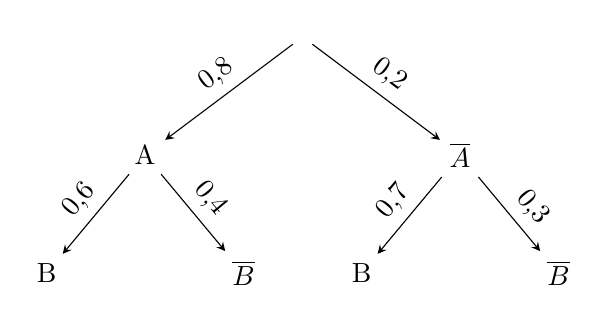
\begin{tikzpicture}[
						level 1/.style={sibling distance=4cm,level  distance=1.5cm},
						level 2/.style={sibling  distance=2.5cm,level distance=1.5cm},
						level  3/.style={sibling distance=1.5cm,level distance=1.5cm},
						 ethicknode/.style={font=\small},
						edge  from parent/.style={draw,-{stealth}},
						 ethickpath/.style={font=\tiny},
						 probability/.style={midway,above,sloped}]
					\node  {}
						 child {node {A}
						 child {node {B}
						edge from parent node [pos=0.5,above,sloped] {0{,}6} 
					} 
						child  {node {$\overline{B}$}
						edge from parent node [pos=0.5,above,sloped] {0{,}4} 
					 }
						edge  from parent node [pos=0.5,above,sloped] {0{,}8}
					} 
						child {node {$\overline{A}$} 
						child {node {B} 
						edge from  parent node [pos=0.5,above,sloped] {0{,}7}
					 }
						child  {node {$\overline{B}$}
						edge from parent node  [pos=0.6,above,sloped] {0{,}3}
					 }
						edge  from parent node [pos=0.5,above,sloped] {0{,}2}
						}; 
				\end{tikzpicture}
		\end{center}
		\begin{itemchoice}
			 \itemch $\mathrm{P}(A)=0{,}8$.
			\itemch Xác suất để một học sinh đó đỗ đại học với điều kiện học sinh đó chọn tổ hợp D01 là 
			 $$\mathrm{P}(B\mid A)=0{,}6.$$
			\itemch Xác suất để một học sinh đó đỗ đại học đồng thời học sinh đó chọn tổ  hợp D01 là
			$$\mathrm{P}(AB)=\mathrm{P}(A)\cdot\mathrm{P}(B\mid A)=0{,}8\cdot0{,}6=0{,}48=\dfrac{12}{25}.$$ 
			\itemch Xác suất để học sinh đó chọn tổ hợp D01 biết rằng học sinh này đã đỗ đại  học
			 $$\mathrm{P}(A\mid B)=\dfrac{\mathrm{P}(AB)}{\mathrm{P}(B)}=\dfrac{0{,}48}{0{,}8\cdot0{,}6+0{,}2\cdot0{,}7}=\dfrac{24}{31}.$$
		\end{itemchoice}
	} 
\end{ex}

% nguồn: Lop_12_Dai_so_Chuong_6
\begin{ex}%[2D6V1-2]%[ma:5ae023ea]
	Một đội văn nghệ của một trường phổ thông gồm có $45$ học sinh, trong đó có $22$ học sinh nam và $23$ học sinh nữ. Có $28$ bạn biết đánh đàn (trong đó có $12$ nam và $16$ nữ) và $17$ bạn không biết đánh đàn  (trong đó có $10$ nam và $7$ nữ). Chọn ngẫu nhiên một bạn học sinh trong đội văn nghệ. Gọi $A$ là biến cố học sinh được chọn là nam, $B$ là biến cố học sinh được chọn biết đánh đàn.
	 \choiceTF
		{\True $\mathrm{P}(A)=\dfrac{22}{45}$} 
		{\True  $\mathrm{P}(B)=\dfrac{28}{45}$}
		{$\mathrm{P}(A \mid  B)=\dfrac{10}{22}$}
		{$\mathrm{P}\left(B  \mid \overline{A}\right)=\dfrac{7}{17}$}
	\loigiai{ 
		\begin{itemchoice}
			\itemch  Vì $n(\Omega)=45$, $n(A)=22$ nên $\mathrm{P}(A)=\dfrac{22}{45}$.
			\itemch Vì $n(\Omega)=45$, $n(B)=28$  nên $\mathrm{P}(B)=\dfrac{28}{45}$.
			 \itemch Vì $n(A\cap B)=12$, $n(B)=28$ nên $\mathrm{P}(A \mid B)=\dfrac{n(A\cap B)}{n(B)}=\dfrac{12}{28} \neq \dfrac{10}{22}$.
			\itemch Vì $n\left(B \cap \overline{A}\right)=16$, $n\left(\overline{A}\right)=23$ nên $\mathrm{P}\left(B \mid \overline{A}\right)=\dfrac{n\left(B  \cap \overline{A}\right)}{n\left(\overline{A}\right)}=\dfrac{16}{23} \neq \dfrac{7}{17}$.
		\end{itemchoice}
	 }
\end{ex}

% nguồn: Lop_12_Dai_so_Chuong_6
\begin{ex}%[2D6V1-2]%[ma:4295f031]
	Cho hai biến cố $A$, $B$ có xác suất lần lượt  là $\mathrm{P}( A)=\dfrac{2}{5}$, $\mathrm{P}( B)=\dfrac{3}{5}$ và\break $\mathrm{P}(AB)=\dfrac{1}{5}$.
	\choiceTF 
		{\True Xác suất của biến cố $\overline{A}$ là  $\mathrm{P}(\overline{A})=\dfrac{3}{5}$}
		{Xác suất của biến cố $B$ với điều kiện $A$ là  $\mathrm{P}(B\mid A)=\dfrac{1}{3}$}
		{Xác suất của biến cố  $A\cup B$ là $\mathrm{P}(A\cup B)=1$}
		{\True  Xác suất của biến cố $\overline{A}$ với điều kiện $\overline{B}$ là $\mathrm{P}(\overline{A}\mid\overline{B})=\dfrac{1}{2}$}
	 \loigiai{
		\begin{itemchoice}
			\itemch 
			$\mathrm{P}(\overline{A})=1-\mathrm{P}(A)=\dfrac{3}{5}$. 
			 \itemch
			$\mathrm{P}( B\mid A)=\dfrac{\mathrm{P}(  AB)}{\mathrm{P}(A)}=\dfrac{1}{5}:\dfrac{2}{5}=\dfrac{1}{2}$.
			\itemch 
			$\mathrm{P}(A\cup B)=\mathrm{P}(A)+\mathrm{P}( B)-\mathrm{P}( AB)=\dfrac{2}{5}+\dfrac{3}{5}-\dfrac{1}{5}=\dfrac{4}{5}$. 
			\itemch 
			Ta  có $\mathrm{P}(\overline{A}\mid\overline{B})=1-\mathrm{P}(A\mid\overline{B})=1-\dfrac{\mathrm{P}(A\overline{B})}{\mathrm{P}(\overline{B})}$.\\
			Lại có $\mathrm{P}(A\overline{B})=\mathrm{P}(A)\cdot \mathrm{P}(\overline{B}\mid  A)=\mathrm{P}(A)\cdot(1-\mathrm{P}( B\mid A))=\dfrac{2}{5}\cdot \left(1-\dfrac{1}{2} \right)=\dfrac{1}{5}=0{,}2$.\\
			Mặt  khác $\mathrm{P}(\overline{B})=1-\mathrm{P}( B)=1-\dfrac{3}{5}=\dfrac{2}{5}=0{,}4$.\\
			Do  đó $\mathrm{P}(\overline{A}\mid\overline{B})=1-\dfrac{0{,}2}{0{,}4}=\dfrac{1}{2}$.
		\end{itemchoice}
	} 
\end{ex}


%%%%%%%%%%%%%%%% TRẢ LỜI NGẮN %%%%%%%%%%%%%%%%

% nguồn: Lop_12_Dai_so_Chuong_6
\begin{bt}%[2D6H1-2]%[ma:04def3f2]
	Hai người $A$ và $B$ mỗi người bắn một viên đạn vào cùng mục tiêu độc lập. Giả sử xác suất bắn trúng đích  của $A$ và $B$ lần lượt là $0{,}7$ và $0{,}4$. Giả sử chỉ có một viên đạn trúng đích, tính xác suất để đó là của $B$ (kết quả làm tròn tới hàng phần trăm).
	\shortans{0,22} 
	 \loigiai{
		Gọi $A$, $B$, $C$ lần lượt là biến cố \lq\lq $A$ bắn trúng\rq\rq, \lq\lq $B$ bắn  trúng\rq\rq, \lq\lq có một người bắn trúng\rq\rq.\\
		Ta  có
		$$ \mathrm{P}(B|C) = \dfrac{\mathrm{P}\left(B\overline{A}\right)}{\mathrm{P}(C)}  = \dfrac{\mathrm{P}\left(B\overline{A}\right)}{\mathrm{P}\left(B\overline{A}\right) + \mathrm{P}\left(A\overline{B}\right)} = \dfrac{0{,}4 \cdot 0{,}3}{0{,}4 \cdot 0{,}3 + 0{,}7 \cdot 0{,}4} = 0{,}22. $$
	} 
\end{bt}

% nguồn: Lop_12_Dai_so_Chuong_6
\begin{bt}%[2D6H1-2]%[ma:51c84ee6]
	Một phòng khám có $2$ bác sĩ, $4$ y tá và $1$ hộ lí. Chọn ra ngẫu nhiên đồng thời $3$ người từ phòng khám đó. Tính xác suất để cả $3$  người đều là y tá, biết rằng trong đó không có bác sĩ nào.
	\shortans{0,4} 
	\loigiai{ 
		Chọn $3$ người từ phòng khám mà không có bác sĩ,  có $\mathrm{C}_5^3=10$.\\
		Gọi biến  cố $A$ là $3$ người được chọn đều là y tá. Ta có $n(A)=\mathrm{C}_4^3=4$.\\
		Vậy xác suất của $A$  là $\mathrm{P}(A)=\dfrac{4}{10}=0{,}4$.
	 }
\end{bt}

% nguồn: Lop_12_Dai_so_Chuong_6
\begin{bt}%[2D6H1-2]%[ma:cc85b579]
	Xác suất bắn trúng đích của xạ thủ hạng I là  $0{,}8$ và của xạ thủ hạng II là $0{,}7$. Chọn ngẫu nhiên $1$ xạ thủ từ một nhóm gồm $4$ xạ thủ hạng I và $6$ xạ thủ hạng II. Xạ thủ này bắn một viên đạn và viên đạn đó trúng mục tiêu, tính xác suất để đó là xạ thủ hạng I (kết quả làm tròn đến hàng phần trăm).
	\shortans{0,43} 
	 \loigiai{
		Gọi $A$ là biến cố \lq \lq Xạ thủ được chọn thuộc hạng I\rq\rq, $C$ là biến cố \lq\lq Xạ thủ bắn  trúng mục tiêu\rq\rq. Ta cần tính $\mathrm{P}(A \mid C)$.\\
		 Ta có $\mathrm{P}(A \mid C)=\dfrac{\mathrm{P}(C \mid A) \mathrm{P}(A)}{\mathrm{P}(C \mid A) \mathrm{P}(A)+\mathrm{P}(C \mid \overline{A}) \mathrm{P}(\overline{A})}=\dfrac{0{,}8\cdot 0{,}4}{0{,}8\cdot 0{,}4+0{,}7\cdot 0{,}6}=\dfrac{16}{37} \approx 0{,}43$.
	} 
\end{bt}

% nguồn: Lop_12_Dai_so_Chuong_6
\begin{bt}%[2D6H1-2]%[ma:d5ecc6cf]
	Một công ty bảo hiểm nhận thấy có $51\%$ số người mua bảo hiểm ô tô là nam, và có $33\%$ số người mua bảo hiểm ô tô là nam trên $50$ tuổi. Biết một người mua bảo hiểm ô tô  là nam, tính xác suất người đó trên $50$ tuổi (làm tròn đến hàng phần trăm).
	\shortans{} 
	\loigiai{Gọi $A$ là biến cố \lq\lq Người mua bảo hiểm ô tô là nam\rq\rq, $B$ là biến cố \lq\lq Người mua bảo hiểm ô tô trên $50$ tuổi\rq\rq. Ta cần  tính $\mathrm{P}(B\mid A)$.\\
		Do có $51\%$ số  người mua bảo hiểm ô tô là nam nên $\mathrm{P}(A) = 0{,}51$.\\
	Do có $33\%$ số người mua bảo hiểm ô tô là nam trên $50$ tuổi nên $\mathrm{P}(AB) = 0{,}33$.\\ Vậy $$\mathrm{P}(B\mid A) = \dfrac{\mathrm{P}(AB) }{\mathrm{P}(A) } = \dfrac{0{,}33}{0{,}51} = \dfrac{11}{17} \approx 0{,}65.$$} 
\end{bt}

% nguồn: Lop_12_Dai_so_Chuong_6
\begin{bt}%[2D6H1-2]%[ma:4ea0744e]
	Gieo con xúc xắc cân đối và đồng chất một lần. Gọi $A$ là biến cố xuất hiện mặt $1$ chấm, $B$ là biến cố xuất hiện mặt  lẻ chấm. Tính xác suất có điều kiện $\mathrm{P}(A|B)$. (kết quả làm tròn đến hàng phần trăm).
	 \shortans{0,33}
	 \loigiai{
		Không gian mẫu $\Omega =  \{1, 2, 3, 4, 5, 6\}$, $n(\Omega) = 6$.\\
		Biến cố $A$: \lq\lq xuất hiện mặt $1$ chấm\rq\rq $\Rightarrow A = \{1\}$,  $n(A) = 1$.\\
		Biến cố $B$: \lq\lq xuất hiện mặt lẻ chấm\rq\rq  $\Rightarrow B = \{1, 3, 5\}$, $n(B) = 3$.\\
		$A  \cap B = \{1\}$, $n(A \cap B) = 1$.\\
		Xác suất của $B$ là $\mathrm{P}(B) = \dfrac{n(B)}{n(\Omega)}  = \dfrac{3}{6} = \dfrac{1}{2}$.\\
		 Xác suất của $A \cap B$ là $\mathrm{P}(A \cap B) = \dfrac{n(A \cap B)}{n(\Omega)} = \dfrac{1}{6}$.\\
		Xác suất có điều kiện $\mathrm{P}(A|B) =  \dfrac{\mathrm{P}(A \cap B)}{\mathrm{P}(B)} = \dfrac{\dfrac{1}{6}}{\dfrac{1}{2}} = \dfrac{1}{3} \approx 0{,}33$.
	} 
\end{bt}

% nguồn: Lop_12_Dai_so_Chuong_6
\begin{bt}%[2D6H1-2]%[ma:9626c415]
	Trong kì kiểm tra môn Toán của một trường THPT  có $400$ học sinh tham gia, trong đó có $190$ học sinh nam và $210$ học sinh nữ. Khi công bố kết quả của kì kiểm tra đó, có $100$ học sinh đạt điểm giỏi, trong đó có $48$ học sinh nam và $52$ học sinh nữ. Chọn ra ngẫu nhiên một học sinh trong số $400$ học sinh đó. Tính xác suất để học sinh được chọn ra đạt điểm giỏi, biết rằng học sinh đó là nữ (làm tròn kết quả đến hàng phần trăm).
	 \shortans{0,25}
	 \loigiai{
		\begin{center}
			\begin{tikzpicture}[scale=.4,font=\footnotesize,line join=round,line cap=round,>=stealth]
					\coordinate (O) at  (2,-1);
					\begin{scope}[ethicknode/.style={circle,draw,fill=red!10}]
						\node (A) at (9,2) {$A$}; 
						\node (B)  at (9,-4) {$\overline{A}$};
						\node (C) at (16,4)  {$B$};
						\node (D) at (16,0) {$\overline{B}$}; 
						 \node (E) at (16,-2.5) {$B$};
						\node (F) at (16,-6.5) {$\overline{B}$}; 
					\end{scope}
					 \node at (A.south) [below=2pt] {nam};
					\node  at (C.east) [right=2pt] {Học sinh đạt điểm giỏi};
					\node at (D.east) [right=2pt] {Học sinh  đạt điểm không giỏi};
					\node  at (B.south) [below=2pt] {nữ};
					\node at (E.east) [right=2pt] {Học sinh đạt  điểm giỏi};
					\node at (F.east) [right=2pt] {Học sinh đạt  điểm không giỏi};
					\draw[->] (O)--(A) node[midway,above,yshift=5pt]{$\dfrac{190}{400}=0{,}475$}; 
					\draw[->] (A)--(C) node[midway,above]{$\dfrac{48}{190}=0{,}2526$}; 
					 \draw[->] (A)--(D) node[midway,below]{$\dfrac{142}{190}=0{,}7474$};
					\draw[->] (O)--(B)  node[midway,below,yshift=-10pt]{$0{,}525$};
					\draw[->]  (B)--(E) node[midway,above,yshift=-5pt]{$\dfrac{52}{210}=0{,}2476$};
					\draw[->] (B)--(F) node[midway,below]{$\dfrac{158}{210}=0{,}7524$}; 
				\end{tikzpicture}
		\end{center}
		Gọi biến cố 
		\begin{itemize}
			\item $A$: học sinh được chọn là nam. 
			\item $\overline{A}$: học sinh  được chọn là nữ.
			\item  $B$: học sinh được chọn đạt điểm giỏi.
		\end{itemize}
		 Theo sơ đồ cây, ta có
		\begin{align*}
			\mathrm{P}(\overline{A}) &= \dfrac{210}{400} = 0{,}525,  \\
			P\left(B|\overline{A}\right) &= \dfrac{52}{210} = 0{,}2476\approx 0{,}25. 
		\end{align*}
	 }
\end{bt}

% nguồn: Lop_12_Dai_so_Chuong_6
\begin{bt}%[2D6H1-2]%[ma:ef0810d9]
	Tỉ lệ người nghiện thuốc lá ở một vùng là  $30\%$. Biết tỉ lệ viêm họng trong số người nghiện thuốc lá là $a\%$ còn người không nghiện là $40\%$. Gặp ngẫu nhiên một người trong vùng thì xác suất để người đó nghiện thuốc và bị viêm họng bằng $0{,}21$; xác suất để người đó không nghiện thuốc và bị viêm họng là $b\%$. Tính $a+b$.
	\shortans{98} 
	 \loigiai{
		Gọi $A$: \lq\lq Người nghiện thuốc lá\rq\rq.\\ 
		$B$: \lq\lq  Người bị viêm họng\rq\rq.\\
		Khi đó $AB$: \lq\lq Người nghiện  thuốc và bị viêm họng\rq\rq.\\
		$\overline{A}B$: \lq\lq Người không  nghiện thuốc và bị viêm họng\rq\rq.\\
		Theo đề bài ta có $\mathrm{P}(A)=30\%$; $\mathrm{P}(B|A)=a\%$ và $\mathrm{P}(AB)=0{,}21$ nên theo công  thức xác suất có điều kiện ta được $\mathrm{P}(B|A)=\dfrac{\mathrm{P}(AB)}{\mathrm{P}(A)} \Leftrightarrow a\% = \dfrac{0{,}21}{30\%} = 70\%$.\\
		Tương tự: $\mathrm{P}\left(\overline{A}\right)=1-30\%=70\%$; $\mathrm{P}\left(B|\overline{A}\right)=40\%$ và $\mathrm{P}\left(\overline{A}B\right)=b\%$ nên theo công thức xác suất có điều kiện ta được: $\mathrm{P}\left(B|\overline{A}\right)=\dfrac{\mathrm{P}\left(\overline{A}B\right)}{\mathrm{P}\left(\overline{A}\right)} \Leftrightarrow 40\% = \dfrac{b\%}{70\%} \Leftrightarrow  b\% = 28\%$.\\
		Vậy  $a+b=98$.
	} 
\end{bt}

% nguồn: Lop_12_Dai_so_Chuong_6
\begin{bt}%[2D6H1-2]%[ma:8bee7a14]
	Lớp 12A có $50$ học sinh, trong đó có $25$ học sinh thích môn Vật lý, $22$ học sinh thích môn Hóa học, và $18$ học sinh không thích môn  nào trong hai môn trên. Chọn ngẫu nhiên $1$ học sinh. Tính xác suất chọn được học sinh thích môn Vật lý, biết rằng học sinh đó thích môn Hóa học (kết quả làm tròn đến hàng phần trăm).
	\shortans{0,68} 
	\loigiai{ 
		Gọi $A$: \lq\lq Học sinh thích môn Vật lý\rq\rq; $B$: \lq\lq Học sinh thích môn Hóa học\rq\rq.\\ 
		Ta có $n(A\cup  B)=n(A)+n(B)-n(A.B)\Rightarrow n\left(A.B\right)=25+22-32=15$.\\
	 Suy ra $P(A|B)=\dfrac{n(A.B)}{n(B)}=\dfrac{15}{22}\approx 0{,}68$.}
\end{bt}

% nguồn: Lop_12_Dai_so_Chuong_6
\begin{bt}%[2D6H1-2]%[ma:5a3911eb]
	Cho hai biến cố $A$, $B$  có $P(A)=0{,}4$; $\mathrm{P}(B)=0{,}6$, $\mathrm{P}(AB)=0{,}3$. Tính $\mathrm{P}\big(\overline{A} \mid B\big)$
	 \shortans{0,5}
	\loigiai{ 
		 Ta có
		 \allowdisplaybreaks
		\begin{eqnarray*}
			\mathrm{P}\big(\overline{A} \mid  B\big) &=& 1-\mathrm{P}(A \mid B) \\
			&=& 1-\dfrac{\mathrm{P}(AB)}{\mathrm{P}(B)}\\ 
			 &=& 1-\dfrac{0{,}3}{0{,}6}=0{,}5.
		\end{eqnarray*}
	} 
\end{bt}

% nguồn: Lop_12_Dai_so_Chuong_6
\begin{bt}%[2D6H1-2]%[ma:7375d187]
	Một bình đựng $50$ viên  bi kích thước, chất liệu như nhau, trong đó có $30$ viên bi xanh và $20$ viên bi trắng. Lấy ngẫu nhiên ra một viên bi, rồi lại lấy ngẫu nhiên ra một viên bi nữa. Tính xác suất để lấy được một viên bi xanh ở lần thứ nhất và một viên bi trắng ở lần thứ hai (kết quả làm tròn đến hàng phần trăm).
	 \shortans{0,41}
	\loigiai{ 
		Gọi $A$ là biến cố: “Lấy được một viên bi xanh ở lần thứ nhất”.\\ 
		Gọi $B$ là biến cố: “Lấy được một viên bi trắng  ở lần thứ hai”.\\
		Ta cần tính xác suất $\mathrm{P}(A\cap B)$.\\ 
		Theo công thức nhân xác  suất $\mathrm{P}(A\cap B)=\mathrm{P}(A)\cdot\mathrm{P}(B|A)$.\\
		Vì có $30$ viên bi xanh trong tổng  số $50$ viên bi nên $\mathrm{P}(A)=\dfrac{30}{50}=\dfrac{3}{5}$.\\
		Nếu $A$ đã xảy ra, tức là một viên bi xanh đã được lấy ra ở lần thứ nhất, thì còn lại trong bình $49$ viên bi trong đó  số viên bi trắng là $20$, do đó $\mathrm{P}(B|A)=\dfrac{20}{49}$.\\
		Vậy xác suất cần tìm là $\mathrm{P}(A\cap B)=\mathrm{P}(A)\cdot\mathrm{P}(B|A)=\dfrac{3}{5}\cdot\dfrac{20}{49}=\dfrac{12}{29}\approx  0{,}41$.
	} 
\end{bt}

% nguồn: Lop_12_Dai_so_Chuong_6
\begin{bt}%[2D6H1-2]%[ma:b0e6cedc]
	Trong một cộng đồng $X$ có tỉ lệ mắc ung thư là $0{,}02$. Biết rằng xác suất xét nghiệm dương tính là $0{,}95$ nếu người đó mắc ung thư và $0{,}03$ nếu người đó không mắc ung thư. Tính  xác suất khi chọn ngẫu nhiên một người trong cộng đồng $X$ bị ung thư nếu người này cho kết quả xét nghiệm dương tính. (Kết quả tính biểu diễn dưới dạng phần trăm, làm tròn đến chữ số hàng phần chục).
	 \shortans{39,3}
	 \loigiai{
		Gọi $A$ là  biến cố người được chọn bị ung thư, $B$ là biến cố người được chọn cho kết quả dương tính.\\
		Khi  đó\\
		+ $B\cap A$ là biến cố người được chọn có kết quả xét nghiệm dương tính và bị  ung thư,\\
		+ $B\cap \overline{A}$ là biến cố người được chọn có kết quả xét nghiệm dương tính và  không bị ung thư.\\
		Mặt khác\\ 
		+ $\mathrm{P}(B|A)$ là xác suất người được chọn có kết quả dương tính khi người được chọn bị  ung thư,\\
		+ $\mathrm{P}\left(B|\overline{A} \right)$ là xác suất người được chọn có  kết quả dương tính khi người được chọn không bị ung thư.\\
		Ta có $\mathrm{P}(A)=0{,}02$, $\mathrm{P}(B|A)=0{,}95$ và $\mathrm{P}\left(B|\overline{A}  \right)=0{,}03$.\\
		Lúc này ta có  $\mathrm{P}(B\cap A)=\mathrm{P}(B|A)\mathrm{P}(A)=0{,}95\cdot 0{,}02=0{,}019$.\\
		Và $\mathrm{P}\left(B\cap \overline{A}\right)=\mathrm{P}\left(B|\overline{A}\right)\mathrm{P}\left(\overline{A}\right)=0{,}03\cdot  0{,}98=0{,}0294$.\\
		Suy ra $\mathrm{P}(B)=\mathrm{P}(B\cap A)+\mathrm{P}\left(B\cap \overline{A}\right)=0{,}0484=4{,}84\%$.\\ 
		Do đó $\mathrm{P}(A|B)=\dfrac{\mathrm{P}(A\cap B)}{\mathrm{P}(B)}=\dfrac{0{,}019}{0{,}0484}\approx  0{,}393=39,3\%$.
	} 
\end{bt}

% nguồn: Lop_12_Dai_so_Chuong_6
\begin{bt}%[2D6H1-2]%[ma:630dfb13]
	Trong hội thảo, xác suất chọn được một người trình bày báo cáo bằng tiếng Anh là $0{,}6$. Xác suất để chọn được một người trình bày là nữ là $0{,}4$. Xác suất để chọn được  một người trình bày báo cáo bằng tiếng Anh biết người đó là nữ là $0{,}3$. Tính xác suất để chọn được một người là nữ sao cho người đó có thể trình bày báo cáo bằng tiếng Anh.
	 \shortans{0,2}
	 \loigiai{
		Gọi $A$ là biến cố \lq\lq Chọn được một người là nữ\rq\rq; $B$ là biến cố \lq\lq Chọn được một người biết trình bày  báo cáo bằng tiếng Anh\rq\rq.\\
		Từ dữ kiện  đề bài ta có $\mathrm{P}(B)=0{,}6$; $\mathrm{P}(A)=0{,}4$; $\mathrm{P}(B\mid A)=0{,}3$.\\
		Ta có $\mathrm{P}(B)\cdot\mathrm{P}(A\mid  B)=\mathrm{P}(A)\cdot\mathrm{P}(B\mid A)$, suy ra
		 $$\mathrm{P}(A\mid B)=\dfrac{\mathrm{P}(A)\cdot\mathrm{P}(B\mid A)}{\mathrm{P}(B)}=\dfrac{0{,}4\cdot0{,}3}{0{,}6}=0{,}2.$$
		Vậy xác suất để chọn được một người là nữ sao  cho người đó có thể trình bày báo cáo bằng tiếng Anh là $0{,}2$.
	 }
\end{bt}

% nguồn: Lop_12_Dai_so_Chuong_6
\begin{bt}%[2D6H1-2]%[ma:dee16b10]
	Gieo con xúc xắc cân đối và đồng chất một lần. Gọi $A$ là biến  cố xuất hiện mặt $1$ chấm và $B$ là biến cố xuất hiện mặt lẻ chấm. Tính xác suất có điều kiện $\mathrm{P} (A\mid B)$ (kết quả làm tròn đến hàng phần trăm).
	\shortans{0,33} 
	 \loigiai{
		Ta có $\mathrm{P} (B)=\dfrac{3}{6}=\dfrac{1}{2}$; $\mathrm{P}(AB)=\dfrac{1}{6}$; $\mathrm{P} (A\mid B) =\dfrac{\mathrm{P} (AB)}{\mathrm{P} (B)}=\dfrac{1}{3}\approx 0{,}33$. 
	} 
\end{bt}

% nguồn: Lop_12_Dai_so_Chuong_6
\begin{bt}%[2D6H1-2]%[ma:588125c3]
	Bạn Minh làm hai bài tập kế tiếp. Xác suất Minh làm đúng  bài thứ nhất là $0{,}7$. Nếu Minh làm đúng bài thứ nhất thì khả năng làm đúng bài thứ hai là $0{,}8$ nhưng nếu Minh làm sai bài thứ nhất thì khả năng làm đúng bài thứ hai là $0{,}2$. Tính xác suất để Minh làm đúng bài thứ nhất biết rằng Minh làm đúng bài thứ hai (làm tròn kết quả đến hàng phần chục).
	\shortans{0,9} 
	\loigiai{ 
		Gọi $A$ là  biến cố: \lq\lq Minh làm đúng bài thứ nhất\rq\rq, theo đề bài ta có $\mathrm{P}(A)=0{,}7$.\\
		Gọi $B$ là biến cố: \lq\lq Minh làm đúng  bài thứ hai\rq\rq, theo đề bài ta có $\mathrm{P}(B|A)=0{,}8$; $\mathrm{P}\left(B|\overline{A}\right)=0{,}2$.\\
		Gọi C là biến cố \lq\lq Minh làm đúng bài thứ nhất biết rằng Minh làm  đúng bài thứ hai\rq\rq, ta có
		$$  \mathrm{P}(C)=\mathrm{P}(A|B)=\dfrac{\mathrm{P}(AB)}{\mathrm{P}(B)}=\dfrac{\mathrm{P}(BA)}{\mathrm{P}(B)}=\dfrac{\mathrm{P}(B|A)\mathrm{P}(A)}{\mathrm{P}(B)}. $$
		Theo đề bài ta có $\mathrm{P}(A\cup B)=\mathrm{P}(A)+\mathrm{P}(B)-\mathrm{P}(AB)=\mathrm{P}(A)+\mathrm{P}(B)-\mathrm{P}(B|A)\mathrm{P}(A)$.\\ 
		 Mặt khác $\mathrm{P}(A\cup B)=1-\mathrm{P}\left(\overline{A}\overline{B}\right)=1-\mathrm{P}\left(\overline{B}|\overline{A}\right)\mathrm{P}\left(\overline{A}\right)=1-0{,}8\cdot 0{,}3=0{,}76$.
		$$ \mathrm{P}(B)=\mathrm{P}(A\cup  B)-\mathrm{P}(A)+\mathrm{P}(B|A)\mathrm{P}(A)=0{,}76-0{,}7+0{,}8\cdot 0{,}7=0{,}62. $$
		 Vậy $\mathrm{P}(C)=\dfrac{\mathrm{P}(B|A)\mathrm{P}(A)}{\mathrm{P}(B)}=\dfrac{0{,}8\cdot 0{,}7}{0{,}62}=\dfrac{28}{31}\approx 0{,}9$.
	} 
\end{bt}

% nguồn: Lop_12_Dai_so_Chuong_6
\begin{bt}%[2D6H1-2]%[ma:ec78eda9]
	Gieo hai con xúc xắc cân đối, đồng chất. Tính xác suất để tổng số chấm xuất hiện trên hai con xúc xắc lớn hơn hoặc bằng $10$, nếu biết rằng có ít nhất một con đã ra mặt $5$ chấm (kết quả làm tròn  đến hàng phần trăm).
	 \shortans{0,27}
	\loigiai{ 
		Gọi $A$  là biến cố: \lq\lq ít nhất một con đã ra mặt $5$ chấm\rq\rq.\\
		Gọi $B$ là biến  cố: \lq\lq tổng số chấm xuất hiện trên hai con xúc xắc lớn hơn hoặc bằng $10$\rq\rq.\\
		Ta  có $\mathrm{P}(A)=1-\mathrm{P}\left(\overline{A}\right)=1-\left(\dfrac{5}{6}\right)^{2}=\dfrac{11}{36}$.\\
		Biến cố  $B$ có các trường hợp $(4;6),(6;4),(5;5),(5;6),(6;5),(6;6)$.\\
		Biến cố $A\cap B$ có $3$ trường hợp xảy ra: $(5;5),(5;6),(6;5)$ có xác suất là $\mathrm{P}(A\cap  B)=\dfrac{3}{36}$.\\
		 Vậy $\mathrm{P}(B|A)=\dfrac{\mathrm{P}(A\cap B)}{\mathrm{P}(A)}=\dfrac{\dfrac{3}{36}}{\dfrac{11}{36}}=\dfrac{3}{11}\approx 0{,}27$.
	} 
\end{bt}

% nguồn: Lop_12_Dai_so_Chuong_6
\begin{bt}%[2D6H1-2]%[ma:6c7fcac7]
	Trong một cuộc khảo sát về sở thích thể thao, $80\%$ người tham gia thích bóng đá, $55\%$ thích bóng rổ và $42\%$ thích cả hai môn  thể thao đó. Chọn ngẫu nhiên một người tham gia khảo sát, tính xác suất để một người được chọn thích bóng rổ, biết người đó đã thích bóng đá (kết quả làm tròn đến hàng phần trăm).
	 \shortans{0,53}
	\loigiai{ 
		Gọi $A$ là biến cố \lq\lq Người được chọn thích  bóng đá\rq\rq\, và $B$ là biến cố \lq\lq Người được chọn thích bóng rổ\rq\rq.\\
		Khi đó $\mathrm{P}(A)=0{,}8$, $\mathrm{P}(B)=0{,}55$ và  $\mathrm{P}(AB)=0{,}42$.\\
		Khi đó xác suất để một người được chọn thích bóng rổ biết người  đó thích bóng đá là
		\[\mathrm{P}(B|A)=\dfrac{\mathrm{P}(AB)}{\mathrm{P}(A)}=\dfrac{0{,}42}{0{,}8}\approx 0{,}53.\] 
	} 
\end{bt}

% nguồn: Lop_12_Dai_so_Chuong_6
\begin{bt}%[2D6H1-2]%[ma:06c1b1c1]
	Một  thùng thăm đựng $50$ thẻ giảm giá cho nhân viên có kích thước, chất liệu như nhau, trong đó có $30$ thẻ xanh và $20$ thẻ trắng. Lấy ngẫu nhiên ra một thẻ, rồi lại lấy ngẫu nhiên ra một thẻ nữa. Tính xác suất để lấy được một thẻ xanh ở lần thứ nhất và một thẻ trắng ở lần thứ hai? (kết quả được làm tròn đến hàng phần trăm). \shortans{0,24}
	\loigiai{ 
		Gọi $A$ là biến cố \lq \lq lấy được một thẻ xanh ở lần thứ nhất \rq  \rq.\\
		Gọi $B$ là biến cố \lq \lq lấy  được một thẻ trắng ở lần thứ hai\rq \rq.\\
		Vậy $AB$ là biến cố \lq \lq  lấy được một thẻ xanh ở lần thứ nhất và một thẻ trắng ở lần thứ hai\rq \rq.\\
		 Ta có $\mathrm{P}\left(A\right)=\dfrac{30}{50}=\dfrac{3}{5}$.\\
		Sau khi lấy thẻ xanh ở lần thứ nhất số thẻ  còn lại là $49$ thẻ nên $\mathrm{P}(B|A)=\dfrac{20}{49}$.\\
		 Vậy $\mathrm{P}(AB)=\mathrm{P}\left(A\right).\mathrm{P}(B|A)=\dfrac{3}{5}\cdot\dfrac{20}{49}=\dfrac{12}{49}\approx 0{,}24$.
	 }
\end{bt}

% nguồn: Lop_12_Dai_so_Chuong_6
\begin{bt}%[2D6H1-2]%[ma:bb748aff]
	Hộp thứ nhất có $4$ viên bi xanh và $6$  viên bi đỏ. Hộp thứ hai có $4$ viên bi xanh và $4$ viên bi đỏ. Các viên bi có cùng kích thước và khối lượng. Lấy ra ngẫu nhiên một viên bi từ hộp thứ nhất chuyển sang hộp thứ hai. Sau đó lại lấy ngẫu nhiên một viên bi từ hộp thứ hai. Xác suất của biến cố $A$: \lq\lq Viên bi lấy ra từ hộp thứ nhất có màu xanh và viên bi lấy ra từ hộp thứ hai có màu đỏ\rq\rq\ là $\dfrac{a}{b}$ $\left( \dfrac{a}{b} \text{ là phân số tối giản} \right)$. Tính $a+b$.
	\shortans{53} 
	\loigiai{Ta có sơ  đồ hình cây
	\begin{center}
		\begin{tikzpicture} [scale=1,font=\footnotesize,line join= round,line cap =round,>=stealth]
				\node  at (0,4) {Hộp thứ nhất};
				 \node at (4,4) {Hộp thứ hai};
				\node (H1)  at (0,0) {4X,6Đ};
				\node (H2_X) at  (4,2) {5X,4Đ};
				\node (H2_D) at  (4,-2) {4X,5Đ};
				 \node (XX) at (8,3.5) {XX};
				\node  (XD) at (8,0.5) {XĐ};
				 \node (DX) at (8,-0.5) {ĐX};
				\node (DD) at (8,-3.5) {ĐĐ}; 
				\node [right=0.5cm  of XX] {$\dfrac{20}{90}$};
				\node [right=0.5cm of XD]  {$\dfrac{16}{90}$};
				\node [right=0.5cm of  DX] {$\dfrac{24}{90}$};
				\node [right=0.5cm of DD]  {$\dfrac{30}{90}$};
				\draw [->] (H1) -- (H2_X) node [midway,above,sloped]  {X} node [midway,below,sloped] {$\dfrac{4}{10}$};
				\draw [->] (H1) -- (H2_D) node [midway,above,sloped] {Đ} node  [midway,below,sloped] {$\dfrac{6}{10}$};
				\draw [->] (H2_X)  -- (XX) node [midway,above,sloped] {X} node [midway,below,sloped] {$\dfrac{5}{9}$};
				\draw [->] (H2_X) -- (XD) node [midway,above,sloped] {Đ} node [midway,below,sloped] {$\dfrac{4}{9}$}; 
				\draw [->] (H2_D) -- (DX) node  [midway,above,sloped] {X} node [midway,below,sloped] {$\dfrac{4}{9}$};
				\draw [->] (H2_D) -- (DD) node  [midway,above,sloped] {Đ} node [midway,below,sloped] {$\dfrac{5}{9}$};
			\end{tikzpicture}
	\end{center}
	 Vậy ta có $\mathrm{P}(A)=\dfrac{16}{90}=\dfrac{8}{45}\Rightarrow a=8;\ b=45 \Rightarrow a+b=53$.
	 }
\end{bt}

% nguồn: Lop_12_Dai_so_Chuong_6
\begin{bt}%[2D6V1-2]%[ma:f090fd75]
	Một hộp chứa $15$ tấm thẻ cùng loại được đánh số lần lượt từ $1$ đến $15$. Bạn An lấy ra lần lượt $3$ thẻ từ hộp, thẻ lấy ra không được hoàn lại hộp. Tính xác suất của biến cố \lq\lq Lần thứ ba An lấy được thẻ ghi số lẻ, biết rằng lần thứ hai An lấy được thẻ ghi  số chẵn\rq\rq\ (làm tròn kết quả đến hàng phầm trăm).
	\shortans{0,57} 
	\loigiai{ 
		 Gọi $A_i$ là biến cố lần thứ $i$ lấy được thẻ chẵn $(i=1,2,3)$.\\
		Ta  cần tính $\mathrm{P}\left(\overline{A_3}\mid A_2\right)=\dfrac{\mathrm{P}\left(\overline{A_3}A_2\right)}{\mathrm{P}(A_2)}$.
		\begin{itemize}
			 \item $\mathrm{P}(A_1)=\dfrac{7}{15}$, $\mathrm{P}\left(\overline{A_1}\right)=\dfrac{8}{15}$, $\mathrm{P}\left(A_2\mid A_1\right)=\dfrac{6}{14}=\dfrac{3}{7}$, $\mathrm{P}\left(A_2\mid \overline{A_1}\right)=\dfrac{7}{14}=\dfrac{1}{2}$.
			\item $\mathrm{P}\left(A_2\right)=\mathrm{P}\left(A_1\right)\cdot \mathrm{P}\left(A_2\mid A_1\right)+\mathrm{P}\left(\overline{A_1}\right)\cdot  \mathrm{P}\left(A_2\mid \overline{A_1}\right)=\dfrac{7}{15}\cdot \dfrac{3}{7}+\dfrac{8}{15}\cdot \dfrac{1}{2}=\dfrac{7}{15}$.
			 \item $\mathrm{P}\left(\overline{A_3}A_2\right)=\mathrm{P}\left(\overline{A_3}A_2A_1\right)+\mathrm{P}\left(\overline{A_3}A_2\overline{A_1}\right)$.\\
			Sủ dụng tính chất $\mathrm{P}\left(A\right)=\mathrm{P}\left(AA_1\right)+\mathrm{P}\left(A\overline{A_1}\right)$ với $A=\overline{A_3}A_2$.  Suy ra
			\begin{eqnarray*}
				\mathrm{P}\left(\overline{A_3}A_2A_1\right)&=&\mathrm{P}\left(\overline{A_3}\mid A_2A_1\right)\cdot  \mathrm{P}\left(A_2A_1\right)\\
				&=&\mathrm{P}\left(\overline{A_3}\mid A_2A_1\right)\cdot \mathrm{P}\left(A_2\mid A_1\right)\cdot  \mathrm{P}\left(A_1\right)\\
				&=&\dfrac{8}{13}\cdot \dfrac{6}{14}\cdot  \dfrac{7}{15}.\\
				\mathrm{P}\left(\overline{A_3}A_2\overline{A_1}\right)&=&\mathrm{P}\left(\overline{A_3}\mid  A_2\overline{A_1}\right)\cdot \mathrm{P}\left(A_2\overline{A_1}\right)\\
				&=&\mathrm{P}\left(\overline{A_3}\mid  A_2\overline{A_1}\right)\cdot \mathrm{P}\left(A_2\mid \overline{A_1}\right)\cdot \mathrm{P}\left(\overline{A_1}\right)\\
				 &=&\dfrac{7}{13}\cdot \dfrac{7}{14}\cdot \dfrac{8}{15}.
			\end{eqnarray*}
			\item  $\mathrm{P}\left(\overline{A_3}\mid A_2\right)=\dfrac{\mathrm{P}\left(\overline{A_3}A_2\right)}{\mathrm{P}\left(A_2\right)}=\dfrac{\mathrm{P}\left(\overline{A_3}A_2A_1\right)+\mathrm{P}\left(\overline{A_3}A_2\overline{A_1}\right)}{\mathrm{P}\left(A_2\right)}=\dfrac{\dfrac{8}{13}\cdot \dfrac{6}{14}\cdot \dfrac{7}{15}+\dfrac{7}{13}\cdot \dfrac{7}{14}\cdot \dfrac{8}{15}}{\dfrac{7}{15}}$\\
			$\Rightarrow \mathrm{P}\left(\overline{A_3}\mid  A_2\right)=\dfrac{4}{7}\approx 0{,}57$.
		\end{itemize}
	 }
\end{bt}

% nguồn: Lop_12_Dai_so_Chuong_6
\begin{bt}%[2D6V1-2]%[ma:23151461]
	Hộp thứ nhất có $3$ viên bi xanh và $6$ viên bi đỏ. Hộp thứ hai có $3$ viên bi xanh và $7$ viên bi đỏ. Các viên bi có cùng kích thước và khối lượng. Lấy ra ngẫu nhiên $1$ viên bi từ hộp thứ nhất chuyển sang hộp thứ hai. Sau đó lại lấy ra ngẫu nhiên đồng thời $2$ viên bi từ hộp thứ hai. Tính xác suất để $2$ viên  bi lấy ra từ hộp thứ hai là bi đỏ (làm tròn kết quả đến hàng phần trăm).
	 \shortans{0,47}
	\loigiai{ 
		Gọi $A$ là biến cố viên bi lấy ra từ hộp thứ nhất màu đỏ, $B$ là biến cố hai viên bi lấy ra từ hộp thứ $2$ màu đỏ. 
	$$\mathrm{P}(B)=\mathrm{P}(AB)+\mathrm{P}\left(\overline{A}B\right) =\mathrm{P}(A)\cdot\mathrm{P}\left(B \mid A\right) +\mathrm{P}\left(\overline{A}\right)\cdot\mathrm{P}\left(B\mid  \overline{A}\right) =\dfrac{6}{9}\cdot\dfrac{\mathrm{C}_8^2}{\mathrm{C}_{11}^2}+\dfrac{3}{9}\cdot\dfrac{\mathrm{C}_7^2}{\mathrm{C}_{11}^2}\approx 0{,}47.$$}
\end{bt}

% nguồn: Lop_12_Dai_so_Chuong_6
\begin{bt}%[2D6V1-2]%[ma:5a1ec8d7]
	Khảo sát một nhóm $100$ người dùng mạng xã hội, người ta thống kê được rằng $60$ người sử dụng Facebook, $45$ người sử dụng TikTok và $25$ người sử dụng cả Facebook và TikTok. Chọn ngẫu nhiên một người từ nhóm này. Xác  suất để người đó sử dụng TikTok là bao nhiêu, biết rằng người đó đã sử dụng Facebook? (kết quả làm tròn đến hàng phần trăm)
	\shortans{0,42} 
	 \loigiai{
		Gọi $A$ là biến cố \lq\lq người được chọn sử dụng Facebook\rq\rq.\\ 
		Gọi $B$ là biến cố \lq\lq người  được chọn sử dụng TikTok\rq\rq.\\
		Ta có $n(A) = 60$, $n(B)  = 45$.\\
		 $n(A \cap B) = 25$.\\
		Xác suất để người đó sử dụng  TikTok biết rằng người đó đã sử dụng Facebook là
		$$P(B|A)= \dfrac{n(A \cap B)}{n(A)} = \dfrac{25}{60} \approx  0{,}42.$$
	 }
\end{bt}

% nguồn: Lop_12_Dai_so_Chuong_6
\begin{bt}%[2D6V1-2]%[ma:e3d7c3cc]
	Trên mặt bàn có $5$ lá bài  đỏ và $5$ lá bài đen chưa được lật. An thực hiện lật ngẫu nhiên lần lượt từng lá bài, trước khi lật từng lá bài An phải đoán màu của lá bài đó và luôn đoán sao cho xác suất đoán đúng màu của lá bài sắp lật là lớn nhất. Xác suất lần lật bài thứ $3$, An đoán đúng màu của lá bài đó là bao nhiêu? (làm tròn kết quả đến hàng phần trăm).
	\shortans{0,56} 
	 \loigiai{
		Sau $2$ lần lật thẻ ta có $4$ khả năng các cặp thẻ đỏ (R) và đen (B) đã lật là  $RR$; $RB$; $BR$; $BB$.\\
		Khi  đó\\
		$\mathrm{P}(RR) = \dfrac{5}{10} \cdot \dfrac{4}{9} = \dfrac{2}{9}$; 
		$\mathrm{P}(RB) = \dfrac{5}{10} \cdot \dfrac{5}{9} = \dfrac{5}{18}$;  $\mathrm{P}(BR) = \dfrac{5}{10} \cdot \dfrac{5}{9} = \dfrac{5}{18}$; $\mathrm{P}(BB) = \dfrac{5}{10} \cdot \dfrac{4}{9} = \dfrac{2}{9}$.\\
		Gọi $X$ là xác suất đoán đúng lần thứ $3$,  ta có\\
		$\mathrm{P}(X) = \mathrm{P}(RR) \cdot \mathrm{P}(X \mid RR) + \mathrm{P}(RB)\cdot \mathrm{P}(X \mid RB) + \mathrm{P}(BR) \cdot \mathrm{P}(X \mid BR)  + \mathrm{P}(BB)\cdot \mathrm{P}(X \mid BB)$\\
		$\mathrm{P}(X) = \dfrac{2}{9} \cdot \dfrac{5}{8} + \dfrac{5}{18}  \cdot \dfrac{4}{8} + \dfrac{5}{18} \cdot \dfrac{4}{8} + \dfrac{2}{9} \cdot \dfrac{5}{8}\approx 0{,}56$.
	} 
\end{bt}

% nguồn: Lop_12_Dai_so_Chuong_6
\begin{bt}%[2D6V1-2]%[ma:912cd714]
	Nhân dịp nghỉ hè, Đoàn trường A có tổ chức hai đội thanh niên tình nguyện đến hỗ trợ hai xã vùng sâu. Đội thứ nhất có $8$ nam $4$ nữ, đội thứ hai có $7$ nam $3$ nữ. Để phù hợp với công việc tại hai xã, Đoàn trường đã chọn ngẫu nhiên $2$ thành viên của đội thứ nhất điều sang đội thứ hai. Sau khi xếp lại nhân sự, đội thứ hai chọn ngẫu nhiên $2$ đoàn viên của đội mình tham gia hướng dẫn người dân phòng chống bệnh sốt xuất huyết. Gọi xác suất để trong $2$ đoàn viên được chọn ở đội thứ hai có $1$ thành viên từ đội thứ nhất điều sang, biết rằng $2$ đoàn viên được chọn gồm $1$ nam  và $1$ nữ, là $\dfrac{a}{b}$ (với $a$, $b$ là các số nguyên dương, $\dfrac{a}{b}$ tối giản). Tìm $a$.
	\shortans{9218} 
	\loigiai{ 
		Gọi $A$ là biến cố: \lq\lq $2$ người được chọn ($1$  nam, $1$ nữ) có $1$ người là chuyển sang, $1$ người gốc của đội $2$\rq\rq.\\
		Gọi $B$ là biến cố: \lq\lq đội $2$ chọn được $2$ người gồm $1$ nam và $1$ nữ\rq\rq. 
		Ta cần tính $\mathrm{P}(A\mid  B)=\dfrac{\mathrm{P}(A\cap B)}{\mathrm{P}(B)}$.\\
		\textbf{Bước 1.} Ta  xét các trường hợp điều chuyển từ đội ${1}$ sang đội ${2}$ để tìm $\mathrm{P}(A\cap B)$.\\
		Ta cần liệt kê các trường hợp chọn  $2$ người từ đội $1$ sang đội $2$.\\
		 \textbf{Trường hợp 1.} $2$ nam.\\
		Xác suất: $\dfrac{\mathrm{C}_8^2}{\mathrm{C}_{12}^2}=\dfrac{28}{66}$.\\ 
		 Đội $2$ sau khi thêm $2$ nam sẽ có: $9$ nam, $3$ nữ.\\
		Tổng số cách chọn ($1$ nam, $1$ nữ):  $9\times 3=27$.\\
		Trong đó, số cặp có $1$  người mới và $1$ người cũ:
		\begin{itemize}
			\item Nam  mới điều chuyển: $2$ người.
			\item Nam gốc:  $7$ người.
			\item Nữ gốc:  $3$ người.
		\end{itemize}
		Nên có thể chọn: $2$ nam điều chuyển $\times 3$ nữ gốc $=6$ (nam mới, nữ  cũ).\\
		Vậy xác suất trong trường hợp này  để chọn được $1$ người mới và $1$ người cũ là $\dfrac{6}{27}$\\
		 $\Rightarrow \mathrm{P}_{1} =\dfrac{28}{66}\cdot\dfrac{6}{27} =\dfrac{28}{297}$.\\
		\textbf{Trường hợp 2.} $1$ nam,  $1$ nữ.\\
		 Xác suất: $\dfrac{\mathrm{C}_8^1\cdot \mathrm{C}_4^1}{\mathrm{C}_{12}^2}=\dfrac{32}{66}$ \\
		Đội $2$ sau khi thêm $1$  nam, $1$ nữ có: $8$ nam, $4$ nữ.\\
		 Tổng cặp ($1$ nam, $1$ nữ): $8\times 4=32$ \\
		Số cặp gồm $1$ người mới, $1$ người  cũ: \\
		Nam mới $(1)$ × nữ gốc $(3) = 3$ hoặc Nữ mới $(1)$ × nam gốc $(7) =  7$.\\
		Nên tổng số cặp gồm $1$ người mới, $1$ người cũ là $10$ cặp.\\ 
		Vậy xác suất trong trường hợp này để chọn được $1$ người mới và $1$ người cũ là $\dfrac{10}{32}$  \\
		$\Rightarrow \mathrm{P}_{2}=\dfrac{32}{66}\cdot\dfrac{10}{32}=\dfrac{5}{33}$.\\ 
		\textbf{Trường  hợp 3.} $2$ nữ.\\
		Xác suất: $\dfrac{\mathrm{C}_4^2}{\mathrm{C}_{12}^2}=\dfrac{6}{66}$.\\ 
		Đội $2$ sau khi thêm $2$ nữ có:  $7$ nam, $5$ nữ.\\
		Tổng số cách chọn cặp ($1$ nam và $1$ nữ): $7\cdot  5=35$.\\
		Trong đó, số  cặp có $1$ người mới và $1$ người cũ:
		\begin{itemize}
			\item Nữ mới điều chuyển: $2$  người.
			\item Nam gốc:  $7$ người.
			\item Nữ gốc:  $3$ người.
		\end{itemize}
		Nên có thể chọn: $2$ nữ mới điều chuyển $\times  7$ nam gốc $=14$ (nam mới, nữ cũ)\\
		Vậy  xác suất trong trường hợp này để chọn được $1$ người mới và $1$ người cũ là $\dfrac{14}{35}$\\
		$\Rightarrow \mathrm{P}_3=\dfrac{6}{66}\cdot\dfrac{14}{35}=\dfrac{2}{55}$.\\ 
		Tính $\mathrm{P}(A\cap B)  =\mathrm{P}_1+\mathrm{P}_2+\mathrm{P}_3=\dfrac{28}{297}+\dfrac{5}{33}+\dfrac{2}{55}=\dfrac{419}{1\,485}$.\\
		\textbf{Bước 2.} Tính $\mathrm{P}(B)$ (Tổng  xác suất chọn $1$ nam $1$ nữ sau khi điều chuyển).\\
		Ta tính từng trường  hợp điều chuyển rồi nhân với xác suất chọn $1$ nam $1$ nữ trong đội $2$.\\
		\textbf{Trường hợp  1.} $2$ nam.\\
		Xác  suất: $\dfrac{\mathrm{C}_8^2}{\mathrm{C}_{12}^2}=\dfrac{28}{66}$.\\
		Đội $2$ sau  khi thêm $2$ nam có: $9$ nam, $3$ nữ.\\
		Tổng cặp (1 nam và $1$ nữ): $9\times 3=27$ có xác suất là  $\dfrac{27}{66}$
		$\Rightarrow  \mathrm{P}_{B_1}=\dfrac{28}{66}\cdot\dfrac{27}{66}=\dfrac{21}{121}$.\\
		\textbf{Trường hợp  2.} $1$ nam, $1$ nữ.\\
		Xác suất: $\dfrac{\mathrm{C}_8^1\cdot  \mathrm{C}_4^1}{\mathrm{C}_{12}^2}=\dfrac{32}{66}$.\\
		Đội $2$ sau khi thêm $1$ nam, $1$ nữ  có: $8$ nam, $4$ nữ. \\
		Tổng cặp ($1$ nam và  $1$ nữ): $8\times 4=32$ có xác suất là $\dfrac{32}{66}$
		 $\Rightarrow \mathrm{P}_{B_2}=\dfrac{32}{66}\cdot\dfrac{32}{66}=\dfrac{256}{1089}$.\\
		\textbf{Trường  hợp 3.} $2$ nữ.\\
		 Xác suất: $\dfrac{\mathrm{C}_4^2}{\mathrm{C}_{12}^2}=\dfrac{6}{66}$.\\
		Đội $2$ sau khi thêm $2$ nữ có: $7$ nam,  $5$ nữ.\\
		Tổng cặp ($1$ nam và $1$  nữ): $7\times 5=35$ có xác suất là $\dfrac{35}{66}$
		$\Rightarrow  \mathrm{P}_{B_3}=\dfrac{6}{66}\cdot\dfrac{35}{66}=\dfrac{35}{727}$.\\
		Vậy $\mathrm{P}_{B}=\mathrm{P}_{B_1}+\mathrm{P}_{B_2}+\mathrm{P}_{B_3}=\dfrac{21}{121}+\dfrac{256}{1\,089}+\dfrac{35}{727}=\dfrac{995}{2\,178}$.\\ 
		 Kết luận
		$\mathrm{P}(A\mid  B)=\dfrac{\mathrm{P}(A\cap B)}{\mathrm{P}(B)}=\dfrac{\dfrac{419}{1\,485}}{\dfrac{995}{2\,178}}=\dfrac{9\,218}{14\,925}.$ \\
	Vậy $a=9\,218$.} 
\end{bt}

% nguồn: Lop_12_Dai_so_Chuong_6
\begin{bt}%[2D6V1-2]%[ma:7bf7194c]
	Có hai chuồng thỏ. Chuồng thứ nhất có $6$ con thỏ đực và $4$ con thỏ cái. Chuồng thứ hai có $4$ con thỏ đực và $5$ con thỏ cái. Từ chuồng thứ nhất lấy ngẫu nhiên ra $1$ con thỏ bỏ vào chuồng thứ hai, rồi từ chuồng thứ hai lấy ngẫu nhiên ra $3$ con thỏ. Biết trong $3$ con thỏ lấy  ra ở chuồng thứ hai thì số thỏ đực nhiều hơn số thỏ cái. Tính xác suất con thỏ lấy ra ở chuồng thứ nhất là thỏ đực (làm tròn kết quả đến hàng phần trăm).
	 \shortans{0,73}
	\loigiai{ 
		Gọi $A$ là biến cố: \lq\lq con thỏ lấy ra ở chuồng  thứ nhất là thỏ đực\rq\rq.\\
		$B$ là biến cố: \lq\lq $3$ con thỏ lấy ra ở chuồng thứ hai  thì số thỏ đực nhiều hơn số thỏ cái\rq\rq.\\
		\textbf{Trường  hợp 1.} Con thỏ lấy ra từ chuồng thứ nhất là thỏ đực.\\
		Khi đó, chuồng thứ hai có $5$ thỏ đực và $5$ thỏ cái.\ 
		$$\mathrm{P}(A  B)=\dfrac{6}{10}\cdot\dfrac{\mathrm{C}_5^2\cdot \mathrm{C}_5^1+\mathrm{C}_5^3}{\mathrm{C}_{10}^3}=\dfrac{3}{10}.$$
		\textbf{Trường hợp 2.} Con thỏ lấy ra từ chuồng thứ nhất là  thỏ cái.\\
		Khi đó, chuồng thứ hai có $4$ thỏ đực và  $6$ thỏ cái.
		$$\mathrm{P}\left(\overline{A}  B\right)=\dfrac{4}{10}\cdot\dfrac{\mathrm{C}_4^2\cdot \mathrm{C}_6^1+\mathrm{C}_4^3}{\mathrm{C}_{10}^3}=\dfrac{17}{150}.$$
		Do đó,  $\mathrm{P}(B)=\mathrm{P}(AB)+\mathrm{P}\left(\overline{A} B\right)=\dfrac{3}{10}+\dfrac{17}{150}=\dfrac{31}{75}$.\\
	Vậy $\mathrm{P}(A\mid B)=\dfrac{\mathrm{P}(A B)}{\mathrm{P}(B)}=\dfrac{3}{10}\cdot\dfrac{75}{31}=\dfrac{45}{62}\approx  0{,}73$.}
\end{bt}

% nguồn: Lop_12_Dai_so_Chuong_6
\begin{bt}%[2D6V1-2]%[ma:1edbd598]
	Một kỳ thi có hai vòng. Thí  sinh đỗ nếu vượt qua được cả hai vòng. Bạn An tham dự kỳ thi này. Xác suất để An qua vòng $1$ là $0{,}8$. Nếu qua được vòng $1$ thì xác suất để An qua được vòng $2$ là $0{,}7$. An được thông báo báo là bị loại. Tính xác suất để An qua được vòng $1$ nhưng không qua được vòng $2$. (Làm tròn tới hàng phần trăm)
	\shortans{0,55} 
	 \loigiai{
		Gọi  $A$ là biến cố \lq\lq An qua được vòng $1$\rq\rq; $\mathrm{P}\left(A\right)=0{,}8$.\\
		$ B  $ là biến cố \lq\lq An qua được vòng 2\rq\rq; $\mathrm{P}\left(B\mid A\right)=0{,}7 $.\\
		$C$ là  biến cố \lq\lq An đỗ kỳ thi\rq\rq;
		$D$ là biến cố \lq\lq An qua được vòng $1$ nhưng không qua được  vòng $2$\rq\rq.\\
		 Ta có $D=A\overline{B}$.\\
		$ \mathrm{P}\left(\overline{D}\mid\overline{C}\right) = \dfrac{\mathrm{P}\left(\overline{D}\overline{C}\right)}{\mathrm{P}\left(\overline{C}\right)} $.\\ 
		Mặt khác, nếu An qua được vòng 1 nhưng không qua vòng $2$ thì An không đỗ kỳ  thi, nên $\mathrm{P}\left(\overline{C}\mid\overline{D}\right) = 1 $ hay $ \mathrm{P}\left(D\overline{C}\right) = P\left(D\right)\cdot \mathrm{P}\left(\overline{C}\mid D\right) = \mathrm{P}\left(D\right)$.\\
		Vì $ \mathrm{P}\left(D\right) = \mathrm{P}\left(A\overline{B}\right) = \mathrm{P}\left(A\right)\cdot\mathrm{P}\left(\overline{B}\mid A\right) = 0{,}8\cdot0{,}3  = 0{,}24 $.\\
		 $ \mathrm{P}\left(\overline{C}\right) = 1 - \mathrm{P}\left(C\right) = 1 - \mathrm{P}\left(AB\right) = 1 - \mathrm{P}\left(A\right)\cdot\mathrm{P}\left(B\mid A\right) = 1 - 0{,}8\cdot0{,}7 = 0{,}44 $.\\
	Vậy  $\mathrm{P}\left(D|\overline{C}\right)=\dfrac{\mathrm{P}\left(D\overline{C}\right)}{\mathrm{P}\left(\overline{C}\right)} =\dfrac{0{,}24}{0{,}44} \approx 0{,}55 $.}
\end{bt}

% nguồn: Lop_12_Dai_so_Chuong_6
\begin{bt}%[2D6V1-2]%[ma:563bebb5]
	Hộp $1$ chứa $3$ viên bi đỏ, $4$ viên bi xanh và $5$ viên bi vàng. Hộp $2$ chứa $4$ viên bi đỏ, $5$ viên bi xanh và $6$ viên bi vàng (các viên bi chỉ khác nhau về màu sắc). An lấy ngẫu nhiên $3$ viên bi từ hộp $1$ rồi bỏ vào hộp  2, sau đó Bình lấy ngẫu nhiên $3$ bi từ hộp $2$. Tính xác suất để $3$ viên bi An chuyển từ hộp $1$ sang có đúng $2$ màu, biết $3$ viên bi Bình lấy ra có đủ $3$ màu (làm tròn kết quả tới hàng phần trăm).
	 \shortans{0,65}
	\loigiai{ 
		Gọi $A$ là biến cố: $3$ viên bi An chuyển từ hộp $1$ sang  có đúng $2$ màu;\\
		$B$ là biến cố: $3$ viên bi Bình  lấy ra có đủ $3$ màu, khi đó ta cần tính $\mathrm{P}(A\mid B)=\dfrac{\mathrm{P}(A B)}{\mathrm{P}(B)}$.\\
		Gọi $x$, $y$,  $z$ là số bi màu đỏ, xanh, vàng lần lượt mà An lấy, thì xác suất An lấy số bi tương ứng là $\dfrac{\mathrm{C}_3^x\cdot \mathrm{C}_4^y\cdot \mathrm{C}_5^z}{\mathrm{C}_{12}^3}$.\\
		Gọi $m$, $n$, $p$ lần lượt là số bi đỏ, xanh, vàng ở hộp $2$ sau khi An chuyển, thì xác suất Bình lấy được $3$  bi đủ $3$ màu là $\dfrac{m\cdot n\cdot p}{\mathrm{C}_{18}^3}$.
		\begin{center}
		 \resizebox{\linewidth}{!}{
			\begin{tabular}{|lll|l|ccc|c|}
				 \hline
				\multicolumn{3}{|c|}{Số bi An lấy} & \multirow{2}{*}{\begin{tabular}[c]{@{}l@{}}Xác suất An lấy\\số bi tương ứng
			\end{tabular}} & \multicolumn{3}{c|}{\begin{tabular}[c]{@{}l@{}}Số bi ở hộp 2\\sau khi An lấy
		\end{tabular}} & \multirow{2}{*}{\begin{tabular}[c]{@{}l@{}}Xác suất Bình\\lấy đủ 3 màu
	\end{tabular}} \\ \cline{1-3} \cline{5-7}
	\multicolumn{1}{|l|}{Đỏ  (3)} & \multicolumn{1}{l|}{Xanh (4)} & Vàng (5) & & \multicolumn{1}{l|}{Đỏ (4)} & \multicolumn{1}{l|}{Xanh (5)} & Vàng (6) & \\ \hline
	\multicolumn{1}{|c|}{1} & \multicolumn{1}{|c|}{1} & \multicolumn{1}{|c|}{1} & $\dfrac{\mathrm{C}_3^{1} \cdot \mathrm{C}_4^{1} \cdot \mathrm{C}_5^{1}}{\mathrm{C}_{12}^{3}}=\dfrac{3}{11}$ & \multicolumn{1}{|c|}{5} & \multicolumn{1}{|c|}{6} & \multicolumn{1}{|c|}{7} &  $\dfrac{5\cdot6\cdot7}{\mathrm{C}_{18}^{3}}=\dfrac{35}{136}$ \\
	 \hline
	\multicolumn{1}{|c|}{0} & \multicolumn{1}{|c|}{1} & \multicolumn{1}{|c|}{2} & $\dfrac{\mathrm{C}_3^{0} \cdot \mathrm{C}_4^{1} \cdot \mathrm{C}_5^{2}}{\mathrm{C}_{12}^{3}}=\dfrac{2}{11}$ & \multicolumn{1}{|c|}{4} & \multicolumn{1}{|c|}{6}  & \multicolumn{1}{|c|}{8} & $\dfrac{4\cdot6\cdot8}{\mathrm{C}_{18}^{3}}=\dfrac{4}{17}$ \\
	\hline 
	\multicolumn{1}{|c|}{0} & \multicolumn{1}{|c|}{2}  & \multicolumn{1}{|c|}{1} & $\dfrac{\mathrm{C}_3^0 \cdot \mathrm{C}_4^2 \cdot \mathrm{C}_5^1}{\mathrm{C}_{12}^3}=\dfrac{3}{22}$ & \multicolumn{1}{|c|}{4} & \multicolumn{1}{|c|}{7} & \multicolumn{1}{|c|}{7} & $\dfrac{4\cdot7\cdot 7}{\mathrm{C}_{18}^3} =\dfrac{49}{204}$ \\
	 \hline
	\multicolumn{1}{|c|}{1} & \multicolumn{1}{|c|}{0}  & \multicolumn{1}{|c|}{2} & $\dfrac{\mathrm{C}_3^1 \cdot \mathrm{C}_4^0 \cdot \mathrm{C}_5^2}{\mathrm{C}_{12}^3}=\dfrac{3}{22}$ & \multicolumn{1}{|c|}{5} & \multicolumn{1}{|c|}{5} & \multicolumn{1}{|c|}{8} & $\dfrac{5\cdot5\cdot8}{\mathrm{C}_{18}^3}=\dfrac{25}{102}$ \\
	\hline 
	\multicolumn{1}{|c|}{1} & \multicolumn{1}{|c|}{2} & \multicolumn{1}{|c|}{0} & $\dfrac{\mathrm{C}_3^1 \cdot \mathrm{C}_4^2 \cdot \mathrm{C}_5^0}{\mathrm{C}_{12}^3}=\dfrac{9}{110}$ & \multicolumn{1}{|c|}{5} & \multicolumn{1}{|c|}{7} &  \multicolumn{1}{|c|}{6} & $\dfrac{5\cdot6\cdot7}{\mathrm{C}_{18}^3}=\dfrac{35}{136}$ \\
	\hline 
	\multicolumn{1}{|c|}{2} & \multicolumn{1}{|c|}{0} & \multicolumn{1}{|c|}{1} & $\dfrac{\mathrm{C}_3^2  \cdot \mathrm{C}_4^0 \cdot \mathrm{C}_5^1}{\mathrm{C}_{12}^3}=\dfrac{3}{44}$ & \multicolumn{1}{|c|}{6} & \multicolumn{1}{|c|}{5} & \multicolumn{1}{|c|}{7} & $\dfrac{5\cdot6\cdot7}{\mathrm{C}_{18}^3}=\dfrac{35}{136}$ \\
	\hline 
	\multicolumn{1}{|c|}{2} & \multicolumn{1}{|c|}{1} &  \multicolumn{1}{|c|}{0} & $\dfrac{\mathrm{C}_3^2 \cdot \mathrm{C}_4^1 \cdot \mathrm{C}_5^0}{\mathrm{C}_{12}^3}=\dfrac{3}{55}$ & \multicolumn{1}{|c|}{6} & \multicolumn{1}{|c|}{6} & \multicolumn{1}{|c|}{6} & $\dfrac{6\cdot6\cdot6}{\mathrm{C}_{18}^3}=\dfrac{9}{34}$ \\
	 \hline
	\multicolumn{1}{|c|}{3} & \multicolumn{1}{|c|}{0} & \multicolumn{1}{|c|}{0} & $\dfrac{\mathrm{C}_3^3 \cdot \mathrm{C}_4^0 \cdot \mathrm{C}_5^0}{\mathrm{C}_{12}^3}=\dfrac{1}{220}$ & \multicolumn{1}{|c|}{7} & \multicolumn{1}{|c|}{5} & \multicolumn{1}{|c|}{6} &  $\dfrac{5\cdot6\cdot7}{\mathrm{C}_{18}^3}=\dfrac{35}{136}$ \\
	 \hline
	\multicolumn{1}{|c|}{0} & \multicolumn{1}{|c|}{3} & \multicolumn{1}{|c|}{0} & $\dfrac{\mathrm{C}_3^0 \cdot \mathrm{C}_4^3 \cdot  \mathrm{C}_5^0}{\mathrm{C}_{12}^3}=\dfrac{1}{55}$ & \multicolumn{1}{|c|}{5} & \multicolumn{1}{|c|}{8} & \multicolumn{1}{|c|}{6} & $\dfrac{4\cdot6\cdot8}{\mathrm{C}_{18}^3}=\dfrac{4}{17}$ \\
	 \hline
	\multicolumn{1}{|c|}{0} & \multicolumn{1}{|c|}{0} & \multicolumn{1}{|c|}{3} & $\dfrac{\mathrm{C}_3^0 \cdot \mathrm{C}_4^0 \cdot \mathrm{C}_5^3}{\mathrm{C}_{12}^3}=\dfrac{1}{22}$ &  \multicolumn{1}{|c|}{5} & \multicolumn{1}{|c|}{5} & \multicolumn{1}{|c|}{9} & $\dfrac{4\cdot5\cdot9}{\mathrm{C}_{18}^3}=\dfrac{15}{68}$ \\
	\hline 
	\end{tabular}
	} 
	\end{center}
	Xác  suất cần tính bằng
	\begin{center}
		\resizebox{\linewidth}{!}{ 
		$\dfrac{\dfrac{2}{11} \cdot \dfrac{4}{17}+\dfrac{3}{22} \cdot \dfrac{49}{204}+\dfrac{3}{22} \cdot \dfrac{25}{102}+\dfrac{9}{110} \cdot \dfrac{35}{136}+\dfrac{3}{44} \cdot \dfrac{35}{136}+\dfrac{3}{55} \cdot \dfrac{9}{34}}{\dfrac{3}{11} \cdot \dfrac{35}{136}+\dfrac{2}{11} \cdot \dfrac{4}{17}+\dfrac{3}{22} \cdot \dfrac{49}{204}+\dfrac{3}{22} \cdot \dfrac{25}{102}+\dfrac{9}{110} \cdot \dfrac{35}{136}+\dfrac{3}{44} \cdot \dfrac{35}{136}+\dfrac{3}{55} \cdot \dfrac{9}{34}+\dfrac{1}{220} \cdot \dfrac{35}{136}+\dfrac{1}{55} \cdot \dfrac{4}{17}+\dfrac{1}{22} \cdot \dfrac{15}{68}} 
			=\dfrac{4\,847}{7\,410} \approx 0{,}65.$ 
		} 
	\end{center}
} 
\end{bt}

% nguồn: Lop_12_Dai_so_Chuong_6
\begin{bt}%[2D6V1-2]%[ma:80beca28]
	Có hai hộp đựng các viên bi: Hộp $I$ có $6$ bi đỏ và $4$ bi xanh, hộp $II$ có $5$ bi đỏ và $5$ bi xanh (các viên bi có cùng kích thước và khối lượng). Bạn Minh lấy ngẫu nhiên một viên bi từ hộp $I$, bạn Như lấy ngẫu nhiên một viên bi từ hộp $II$. Biết rằng có viên bi đỏ được lấy ra, khi đó xác suất để bạn Như  lấy được viên bi đỏ là $\dfrac{a}{b}$, với $a,b\in {{\mathbb{N}}^*}$ và $\dfrac{a}{b}$ là phân số tối giản. Tính $a-b$.
	 \shortans{-3}
	\loigiai{ 
		Gọi $A$ là biến cố: \lq\lq Bạn Như lấy  được viên bi đỏ\rq\rq. \\
		Gọi $B$ là biến cố: \lq\lq Có viên bi đỏ trong hai  viên được lấy ra\rq\rq.\\
		 Ta cần tìm xác suất $\mathrm{P} (A\mid B)$.\\
		Theo công thức xác suất có điều kiện $\mathrm{P} (A\mid B)=\dfrac{\mathrm{P} (AB)}{\mathrm{P} (B)}=\dfrac{n(AB)}{n(B)}$.\\ 
		Ta có $n(B)=\mathrm{C}_{10}^1\cdot \mathrm{C}_{10}^1-\mathrm{C}_4^1\cdot\mathrm{C}_5^1=80$  (số cách lấy hai viên bi trong đó có ít nhất $1$ bi đỏ).\\
		Và $n(AB)=\mathrm{C}_5^1\cdot\mathrm{C}_{10}^1=50$ (số cách lấy hai viên bi trong đó viên bi của  bạn Như là bi đỏ).\\
		Thay số, ta  được $\mathrm{P} (A\mid B)=\dfrac{50}{80}=\dfrac{5}{8}$.\\
		Vậy $a=5,\,b=8  \Rightarrow a-b=-3$.
	} 
\end{bt}

% nguồn: Lop_12_Dai_so_Chuong_6
\begin{bt}%[2D6V1-2]%[ma:c204cd72]
	Một nhà máy sản xuất pin điện thoại có $2$ dây chuyền sản xuất. Dây chuyền I tạo ra $65\%$ sản phẩm của toàn nhà máy; dây chuyền II tạo ra $35\%$ sản  phẩm của toàn nhà máy. Trong số các sản phẩm được sản xuất từ dây chuyền I có $3\%$ sản phẩm bị lỗi, trong số các sản phẩm được sản xuất từ dây chuyền II có $2\%$ sản phẩm bị lỗi. Chọn ngẫu nhiên một sản phẩm của nhà máy, gọi xác suất để sản phẩm đó là sản phẩm bị lỗi và được sản xuất từ dây chuyền I bằng $P$. Tính $1000 P$.
	 \shortans{195}
	\loigiai{ 
		\begin{center}
			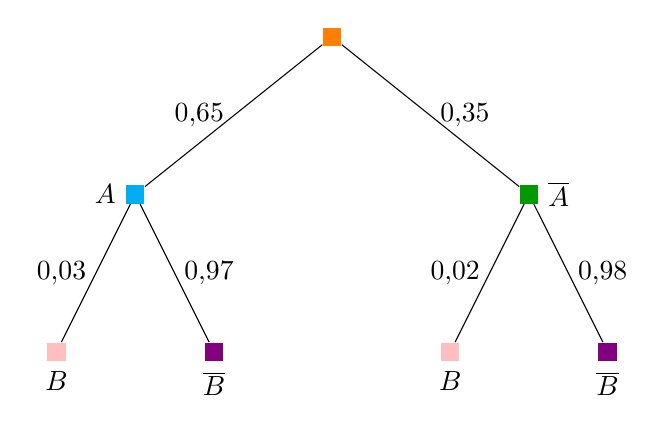
\begin{tikzpicture}
					\tikzstyle{orange_node}=[fill=orange] 
					\tikzstyle{cyan_node}=[fill=cyan] 
					\tikzstyle{green_node}=[fill=green!60!black] 
					\tikzstyle{pink_node}=[fill=pink] 
					\tikzstyle{purple_node}=[fill=violet] 
					\node[orange_node]  (root) at (0,4) {};
					\node[cyan_node,label={left:$A$}] (A) at (-2.5,2) {}; 
					\node[green_node,label={right:$\overline{A}$}]  (Abar) at (2.5,2) {};
					\node[pink_node,label={below:$B$}] (B1) at  (-3.5,0) {};
					\node[purple_node,label={below:$\overline{B}$}] (Bbar1) at  (-1.5,0) {};
					\node[pink_node,label={below:$B$}] (B2)  at (1.5,0) {};
					\node[purple_node,label={below:$\overline{B}$}] (Bbar2) at (3.5,0)  {};
					\draw (root) -- (A) node[midway,left] {$0{,}65$}; 
					\draw (root) -- (Abar) node[midway,right] {$0{,}35$}; 
					\draw (A) -- (B1) node[midway,left] {$0{,}03$}; 
					 \draw (A) -- (Bbar1) node[midway,right] {$0{,}97$};
					\draw  (Abar) -- (B2) node[midway,left] {$0{,}02$};
					\draw (Abar)  -- (Bbar2) node[midway,right] {$0{,}98$};
				\end{tikzpicture}
		\end{center}
		Gọi $A$ là biến cố: \lq\lq Sản phẩm đó được sản xuất từ dây chuyền I\rq\rq; $B$ là biến cố: \lq\lq Sản phẩm đó  bị lỗi\rq\rq.\\
		$\mathrm{P}(A)=0{,}65$, 
		$\mathrm{P}\left(\overline{A}\right)=1-\mathrm{P}(A)=1-0{,}65=0{,}35$.\\ 
		$\mathrm{P}\left(B\mid A\right)$ là xác  suất để sản phẩm bị lỗi biết rằng đó là sản phẩm của dây chuyền I.\\
		$\Rightarrow\mathrm{P}\left(B\mid A\right)=0{,}03$.\\ 
		Theo công thức nhân xác suất ta  có $P=\mathrm{P}(AB)=\mathrm{P}(A)\cdot\mathrm{P}\left(B\mid A\right)=0{,}65\cdot 0{,}3=0{,}195$.\\
	 Vậy $1000 P=195$.}
\end{bt}

% nguồn: Lop_12_Dai_so_Chuong_6
\begin{bt}%[2D6V1-2]%[ma:3e683c78]
	Có $40$ tấm thẻ kích thước  như nhau và đánh số thứ tự lần lượt từ $1$ đến $40$ (mỗi tấm thẻ chỉ ghi một số nguyên dương, hai thẻ khác nhau ghi hai số khác nhau). Một người lần lượt rút hai thẻ (rút không hoàn lại). Tính xác suất lần thứ hai rút được thẻ ghi số nguyên tố.
	 \shortans{0,3}
	 \loigiai{
		Xét các biến  cố:
		\begin{itemize}
			\item $A\colon$ \lq \lq Lần thứ nhất rút  được thẻ ghi số nguyên tố\rq \rq;
			\item $B\colon$ \lq \lq Lần thứ hai rút  được thẻ ghi số nguyên tố\rq \rq.
		\end{itemize}
		Từ $1$ đến $40$ có $12$  số nguyên tố nên $\mathrm{P}(A)=\dfrac{12}{40}=0{,}3$.\\
		Rút được thẻ không phải là số nguyên tố  $\mathrm{P}(\overline{A})=1-0{,}3=0{,}7$.\\
		Vì rút ra không hoàn lại nên lần thứ hai rút được thẻ có ghi  số nguyên tố thì \[\mathrm{P}(B\,|\,A)=\dfrac{11}{39} \text{ và } \mathrm{P}(B|\overline{A})=\dfrac{12}{39}=\dfrac{4}{13}.\]
		 Theo công thức xác suất toàn phần, ta có \[\mathrm{P}(B)=\mathrm{P}(A)\cdot \mathrm{P}(B|A)+\mathrm{P}\left(\overline{A}\right)\cdot \mathrm{P}\left(B|\overline{A}\right)=0{,}3\cdot \dfrac{11}{39}+0{,}7\cdot \dfrac{4}{13}=0{,}3.\]
	} 
\end{bt}

% nguồn: Lop_12_Dai_so_Chuong_6
\begin{bt}%[2D6V1-2]%[ma:6646f41b]
	Một bình đựng $50$ viên bi có kích thước, chất liệu như nhau; trong đó có $30$ viên bi màu đen và $20$ viên bi màu trắng. Lấy ngẫu nhiên ra một viên bi không hoàn lại, rồi lại lấy ngẫu nhiên ra một viên bi nữa. Tính xác suất để lấy được một viên bi màu đen ở lần thứ nhất và một viên bi  màu trắng ở lần thứ hai (kết quả làm tròn đến hàng phần trăm).
	\shortans{0,24} 
	 \loigiai{
		\begin{center}
			\begin{tikzpicture}
					 \tikzstyle{dot}=[circle,fill=blue,inner sep=1.5pt]
					\tikzstyle{labeltext}=[text=red!80!black] 
					\node[dot,label={[labeltext,above]:Gốc}] (O) at (0,0) {}; 
					\node[dot,label={[labeltext,above  left]:$B$}] (B) at (-2.5,-2.5) {};
					\node[dot,label={[labeltext,above right]:$\overline{B}$}] (Bbar) at  (2.5,-2.5) {};
					\node[dot,label={[labeltext,below=0.1]:$A$}] (A1)  at (-4,-5) {};
					\node[dot,label={[labeltext,below=0.1]:$\overline{A}$}]  (Abar1) at (-1,-5) {};
					\node[dot,label={[labeltext,below=0.1]:$A$}]  (A2) at (1,-5) {};
					\node[dot,label={[labeltext,below=0.1]:$\overline{A}$}]  (Abar2) at (4,-5) {};
					\draw[gray] (O)  -- (B) node[midway,above left,labeltext] {$\dfrac{3}{5}$};
					\draw[gray]  (O) -- (Bbar) node[midway,above right,labeltext] {$\dfrac{2}{5}$};
					\draw[gray] (B) --  (A1);
					\draw[gray]  (B) -- (Abar1);
					\draw[gray] (Bbar) --  (A2);
					\draw[gray] (Bbar) -- (Abar2); 
				\end{tikzpicture}
		\end{center}
		Gọi $B$  là biến cố lấy được viên bi đen lần thứ nhất.\\
		Gọi $A$ là  biến cố lấy được viên bi trắng lần thứ hai.\\
		Ta có $\mathrm{P}(B)=\dfrac{3}{5}$ và  $\mathrm{P}\left(\overline{B}\right)=\dfrac{2}{5}$,
		$\mathrm{P}\left(A\mid B\right)=\dfrac{20}{49}$, $\mathrm{P}\left(\overline{A}\mid B\right)=\dfrac{29}{49}$, $\mathrm{P}\left(A\mid\overline{B}\right)=\dfrac{19}{49}$, $\mathrm{P}\left(\overline{A}\mid\overline{B}\right)=\dfrac{30}{49}$.\\ 
	Ta có biến cố $AB$:  \lq\lq lấy được một viên bi màu đen ở lần thứ nhất và một viên bi màu trắng ở lần thứ hai\rq\rq: $\mathrm{P}(A\cdot B)=\mathrm{P}(B)\cdot\mathrm{P}(A\mid B)=\dfrac{3}{5}\cdot\dfrac{20}{49}=\dfrac{12}{49}\approx 0{,}24$.}
\end{bt}

% nguồn: Lop_12_Dai_so_Chuong_6
\begin{bt}%[2D6V1-2]%[ma:f7362148]
	Một người tham gia  trò chơi với ba hộp quà đặc biệt: Hộp màu vàng có $2$ điện thoại iPhone và $3$ tai nghe, hộp màu bạc có $4$ điện thoại iPhone và $1$ tai nghe và hộp màu đồng có $3$ điện thoại iPhone và $2$ tai nghe. Luật chơi được thực hiện qua $2$ bước sau:
	\begin{itemize}
		\item \textbf{Bước 1:} Người chơi chọn ngẫu nhiên một  hộp.
		\item \textbf{Bước 2:} Từ hộp đã chọn, người chơi lấy  ngẫu nhiên 1 món quà
		\begin{itemize}
			\item  Nếu quà là điện thoại iPhone, người chơi được giữ nó và lấy thêm 1 quà nữa từ cùng hộp.
			\item Nếu quà là tai nghe, trò  chơi kết thúc.
		\end{itemize}
	\end{itemize}
	Biết rằng người chơi lấy được hai điện thoại iPhone, tính xác suất để người đó lấy từ hộp màu  bạc (làm tròn kết quả đến hàng phần mười).
	\shortans{0,55} 
	 \loigiai{
		Gọi  $A_1$ là biến cố: \lq \lq Hộp được chọn màu vàng\rq \rq.\\
		$A_2$ là biến cố:  \lq \lq Hộp được chọn màu bạc\rq \rq.\\
		$A_3$ là  biến cố: \lq \lq Hộp được chọn màu đồng\rq \rq.\\
		$B$  là biến cố: \lq \lq Người chơi lấy được hai điện thoại iPhone\rq \rq.\\
		Theo giả  thiết $\mathrm{P}(A_1)=\mathrm{P}(A_2)=\mathrm{P}(A_3)=\dfrac{1}{3}$. Ta cần tính $\mathrm{P}(A_2|B)$.\\
		 Ta có
		\begin{itemize}
			 \item $\mathrm{P}(A_2|B)=\dfrac{\mathrm{P}(A_2B)}{\mathrm{P}\left(B\right)}$.
			\item $\mathrm{P}(A_2B)=\mathrm{P}(B|A_2)\cdot \mathrm{P}(A_2)=\dfrac{4}{5}\cdot\dfrac{3}{4}\cdot\dfrac{1}{3}=\dfrac{1}{5}$. 
			\item $\mathrm{P}\left(B\right)=\mathrm{P}(B|A_1)\cdot \mathrm{P}(A_1)+\mathrm{P}(B|A_2)\cdot \mathrm{P}(A_2)+\mathrm{P}(B|A_3)\cdot  \mathrm{P}(A_3)=\dfrac{1}{3}\cdot\dfrac{2}{5}\cdot\dfrac{1}{4}+\dfrac{1}{3}\cdot\dfrac{4}{5}\cdot\dfrac{3}{4}+\dfrac{1}{3}\cdot\dfrac{3}{5}\cdot\dfrac{2}{3}$.
		\end{itemize}
		 Vậy $\mathrm{P}(A_2|B)=\dfrac{\mathrm{P}(A_2B)}{\mathrm{P}\left(B\right)}=\dfrac{\dfrac{1}{5}}{\dfrac{11}{30}}=\dfrac{6}{11}\approx 0{,}55$.
	 }
\end{bt}

% nguồn: Lop_12_Dai_so_Chuong_6
\begin{bt}%[2D6V1-2]%[ma:74fa2115]
	Có hai hộp đựng bi. Hộp thứ nhất chứa $7$ viên bi màu trắng, $5$ viên bi màu đỏ, hộp  thứ hai chứa $4$ viên bi màu trắng, $6$ viên bi màu đỏ. Lấy ngẫu nhiên $2$ viên bi từ hộp thứ nhất bỏ sang hộp thứ hai, sau đó lấy ngẫu nhiên $3$ viên bi từ hộp thứ hai. Tính xác suất lấy được cả $2$ viên bi thuộc hộp thứ nhất bỏ sang hộp thứ hai, biết rằng $3$ viên bi đó màu trắng (kết quả làm tròn đến hàng phần mười).
	\shortans{0,5} 
	 \loigiai{
		Gọi  $A$ là biến cố \lq\lq Trong $3$ viên bi lấy ra từ hộp hai có $2$ viên bi từ hộp thứ nhất chuyển sang\rq\rq.\\
		Gọi $B$ là biến  cố \lq\lq $3$ viên bi lấy ra từ hộp hai là màu trắng\rq\rq.\\
		Trường hợp 1: $2$ viên bi  từ hộp thứ nhất chuyển sang là $2$ viên bi trắng. Khi đó
		\[\mathrm{P}  (B)=\dfrac{\mathrm{C}_7^2}{\mathrm{C}_{12}^2}\cdot\dfrac{\mathrm{C}_6^3}{\mathrm{C}_{12}^3}=\dfrac{7}{242}.\]
		Trường hợp 2: $2$ viên bi từ hộp thứ  nhất chuyển sang là $2$ viên bi đỏ. Khi đó
		 \[\mathrm{P} (B)=\dfrac{\mathrm{C}_5^2}{\mathrm{C}_{12}^2}\cdot\dfrac{\mathrm{C}_4^3}{\mathrm{C}_{12}^3}=\dfrac{1}{363}.\]
		Trường hợp 3: $2$ viên bi từ hộp thứ nhất chuyển sang là $1$ viên bi trắng  và $1$ viên bi đỏ. Khi đó
		\[\mathrm{P} (B)=\dfrac{\mathrm{C}_7^1\cdot \mathrm{C}_5^1}{\mathrm{C}_{12}^2}\cdot\dfrac{\mathrm{C}_5^3}{\mathrm{C}_{12}^3}=\dfrac{35}{1452}.\] 
		Do đó $\mathrm{P} (A\mid  B)=\dfrac{\mathrm{P} (AB)}{\mathrm{P} (B)}=\dfrac{\dfrac{7}{242}}{\dfrac{27}{484}}=\dfrac{14}{27}\approx 0{,}5$.
	} 
\end{bt}

% nguồn: Lop_12_Dai_so_Chuong_6
\begin{bt}%[2D6V1-2]%[ma:40fd26bd]
	Hiện nay, nước ta đang trong quá trình tinh gọn bộ máy và thực hiện nghị quyết không tổ chức công an cấp huyện. Do vậy, trong đợt điều động cán bộ công an từ huyện về công tác tại cở sở hoặc công tác tại công an tỉnh, phòng tổ chức cán bộ nhận thấy rằng: có $60\%$ cán bộ có nguyện vọng về công tác tại cơ sở là  các xã vùng sâu vùng xa, số còn lại nguyện vọng về công tác tại công an tỉnh.
	\begin{itemize}
		\item Trong số cán bộ có nguyện vọng về công tác tại  cơ sở thì $70\%$ có trình độ đại học và $30\%$ có trình độ trung cấp.
		 \item Trong số cán bộ có nguyện vọng về công an tỉnh thì $80\%$ có trình độ đại học và $20\%$ có trình độ trung cấp.
	\end{itemize}
	Tuy nhiên, năng lực công tác cũng là một yếu tố quan trọng.  Dựa trên hồ sơ đánh giá năng lực:
	\begin{itemize}
		\item Trong số cán bộ có nguyện vọng về cơ sở thì tỷ lệ cán bộ được đánh giá có năng lực \lq\lq Tốt\rq\rq\, trở lên với trình độ đại học là $60\%$  và có trình độ trung cấp là $30\%$.
		\item Trong số cán bộ có nguyện vọng về công tác tại công an tỉnh thì tỷ lệ  cán bộ được đánh giá có năng lực \lq\lq Tốt\rq\rq\, trở lên với trình độ đại học là $85\%$ và với trình độ trung cấp là $25\%$.
	\end{itemize}
	Chọn ngẫu nhiên một cán bộ công an. Tính xác suất để cán bộ này vừa có trình độ đại học, vừa được  đánh giá có năng lực \lq\lq Tốt\rq\rq\, và có nguyện vọng về công tác tại cơ sở là các xã vùng sâu vùng xa. (Kết quả làm tròn đến hàng phần trăm).
	 \shortans{0,25}
	 \loigiai{
		Gọi $A$ là  biến cố: \lq\lq Cán bộ có nguyện vọng về công tác tại cơ sở\rq\rq.\\
		$B$ là biến  cố: \lq\lq Cán bộ vừa có trình độ đại học, vừa được đánh giá năng lực Tốt\rq\rq.\\
		Theo giả thiết, ta có sơ đồ cây  sau
		\begin{center}
			\begin{tikzpicture}[>=stealth]
					\coordinate  (start) at (0,0);
					\coordinate (tinh_branch) at  (2.5,1.5);
					\coordinate (coso_branch)  at (2.5,-1.5);
					\node at  (tinh_branch) [above=0.2,inner sep=1pt] {Tỉnh};
					\node at (coso_branch) [below=0.2,inner  sep=1pt] {Cơ sở};
					 \node (dh1) at (5.5,2.5) {ĐH};
					\node (tc1)  at (5.5,0.5) {TC};
					\node  (dh2) at (5.5,-0.5) {ĐH};
					\node (tc2) at (5.5,-2.5)  {TC};
					\node (tot1) at  (8.5,2.5) {Tốt};
					 \node (tot2) at (8.5,0.5) {Tốt};
					\node (tot3) at  (8.5,-0.5) {Tốt};
					\node (tot4) at (8.5,-2.5)  {Tốt};
					\draw[->] (start) --  (tinh_branch) node[midway,above left,inner sep=2pt] {$0{,}4$};
					\draw[->]  (start) -- (coso_branch) node[midway,below left,inner sep=2pt] {$0{,}6$};
					\draw[->] (tinh_branch) -- (dh1.west)  node[midway,above left,inner sep=2pt] {$0{,}8$};
					\draw[->] (tinh_branch) -- (tc1.west) node[midway,below left,inner sep=2pt] {$0{,}2$}; 
					\draw[->]  (coso_branch) -- (dh2.west) node[midway,above left,inner sep=2pt] {$0{,}7$};
					\draw[->] (coso_branch) -- (tc2.west) node[midway,below  left,inner sep=2pt] {$0{,}3$};
					\draw[->] (dh1.east) -- (tot1.west) node[midway,above,inner  sep=2pt] {$0{,}85$};
					 \draw[->] (tc1.east) -- (tot2.west) node[midway,above,inner sep=2pt] {$0{,}25$};
					\draw[->] (dh2.east) -- (tot3.west)  node[midway,above,inner sep=2pt] {$0{,}6$};
					 \draw[->] (tc2.east) -- (tot4.west) node[midway,above,inner sep=2pt] {$0{,}3$};
				\end{tikzpicture}
		\end{center}
	Vậy $\mathrm{P}(A\cap  B)=0{,}6\cdot 0{,}7\cdot 0{,}6=0{,}252\approx 0{,}25$.}
\end{bt}

% nguồn: Lop_12_Dai_so_Chuong_6
\begin{bt}%[2D6V1-2]%[ma:547eb401]
	Lớp $12A$ có $30$ học sinh, trong đó có $17$ bạn nữ còn lại là nam. Có $3$ bạn tên Minh, trong đó có $1$ bạn nữ và $2$ bạn nam. Thầy giáo gọi  ngẫu nhiên $1$ bạn lên bảng. Xác suất để bạn được gọi tên Minh, nhưng với điều kiện bạn đó là nam bằng $\dfrac{a}{b}$ (với $\dfrac{a}{b}$ là phân số tối giản). Tính giá trị biểu thức $T=a+b$.
	\shortans{15} 
	 \loigiai{Gọi $A$ là biến cố \lq\lq Bạn được gọi tên Minh\rq\rq.\\
		Gọi $B$  là biến cố \lq\lq Bạn được gọi là nam\rq\rq.\\
		Xác suất để thầy giáo gọi bạn đó lên bảng có tên Minh,  nhưng với điều kiện bạn đó nam là $\mathrm{P}\left(A\mid B\right)$.\\
		Ta có $$\mathrm{P}(B) =\dfrac{13}{30};\,\mathrm{P}(A  \cap B) =\dfrac{2}{30}.$$
	Do đó  $$\mathrm{P}(A\mid B) =\dfrac{\mathrm{P}(A \cap B) }{\mathrm{P}(B) }=\dfrac{\dfrac{2}{30}}{\dfrac{13}{30}}=\dfrac{2}{13}.$$}
\end{bt}

% nguồn: Lop_12_Dai_so_Chuong_6
\begin{bt}%[2D6V1-2]%[ma:69489053]
	Bạn An có hai quân xúc xắc $6$ mặt. Một xúc xắc cân đối có xác suất ra các mặt đều như nhau. Xúc xắc còn lại có xác suất ra mặt $6$ là $\dfrac{2}{3}$ và xác suất ra các mặt còn lại bằng nhau. Bạn A chọn ngẫu nhiên một trong hai xúc xắc và tung nó ba lần. Xác suất để lần thứ ba ra mặt $1$ khi biết cả hai lần trước đó đều ra mặt $6$ là $\dfrac{p}{q}$ với $p$, $q$ là các số nguyên dương và  số nguyên tố cùng nhau. Tính $p+q$.
	 \shortans{547}
	\loigiai{ 
		Gọi $A$ là biến cố:  \lq\lq Chọn được con xúc xắc cân đối\rq\rq.\\
		Gọi $\overline{A}$  là biến cố: \lq\lq Chọn được con xúc xắc còn lại\rq\rq.\\
		Gọi $B$ là biến cố: \lq\lq Chọn được lần trước  đều ra mặt $6$ \rq\rq.\\
		Gọi $C$ là  biến cố: \lq\lq Chọn được lần thứ ba ra mặt $1$\rq\rq.\\
		Ta có\\ 
		$\mathrm{P}  (A)=\mathrm{P} (\overline{A})=\dfrac{1}{2}$.\\
		$\mathrm{P} (B)=\dfrac{1}{2}\cdot\dfrac{1}{6}\cdot\dfrac{1}{6}+\dfrac{1}{2}\cdot\dfrac{2}{3}\cdot\dfrac{2}{3}=\dfrac{17}{72}$.\\ 
		$\mathrm{P}  (C\mid B)=\dfrac{\mathrm{P} (CB)}{\mathrm{P} (B)}=\dfrac{\dfrac{1}{2}\cdot\dfrac{1}{6}\cdot\dfrac{1}{6}\cdot\dfrac{1}{6}+\dfrac{1}{2}\cdot\dfrac{2}{3}\cdot\dfrac{2}{3}\cdot\dfrac{1}{15}}{\dfrac{17}{72}}=\dfrac{37}{510}$.\\
		 Suy ra $p=37,\,\,q=510\Rightarrow p+q=547$.
	 }
\end{bt}

% nguồn: Lop_12_Dai_so_Chuong_6
\begin{bt}%[2D6V1-2]%[ma:e07808ea]
	Cho $A$, $B$  là các biến cố của một phép thử $T$. Biết $\mathrm{P}(AB)=0{,}2$; $\mathrm{P}(A\cup B)=0{,}6$; $\mathrm{P}\left(A\mid \overline{B}\right)=0{,}2$. Tính $\mathrm{P}\left(B\mid \overline{A}\right)$ (kết quả làm tròn đến hàng phần trăm).
	\shortans{0,43} 
	 \loigiai{
		Ta  có $\mathrm{P}\left(A\cup B\right)=0{,}6\Rightarrow \mathrm{P}\left(\overline{A}~\overline{B}\right)=0{,}4$.\\
		Lại  có $\mathrm{P}\left(A\mid \overline{B}\right)=1-\mathrm{P}\left(\overline{A}\mid \overline{B}\right)=1-\dfrac{\mathrm{P}\left(\overline{A}~ \overline{B}\right)}{\mathrm{P}\left(\overline{B}\right)}$\\
		$\Rightarrow  \mathrm{P}\left(\overline{B}\right)=\dfrac{\mathrm{P}\left(\overline{A}~ \overline{B}\right)}{1-\mathrm{P}\left(A\mid \overline{B}\right)}=1-\dfrac{0{,}4}{1-0{,}2}=0{,}5$.\\
		 $\Rightarrow \mathrm{P}\left(\overline{B}\right)=0{,}5$.\\
		Mà  $\mathrm{P}\left(A \cup B\right)=\mathrm{P}\left(A\right)+\mathrm{P}\left(B\right)-\mathrm{P}\left(A B\right)$ nên
		\[\mathrm{P}\left(A\right)=\mathrm{P}\left(A \cup  B\right)-\mathrm{P}\left(B\right)+\mathrm{P}\left(A B\right)=0{,}6-0{,}5+0{,}2=0{,}3. \]
		 Vậy $\mathrm{P}\left(B\mid\overline{A}\right)=1-\mathrm{P}\left(\overline{B}\mid\overline{A}\right)=1-\dfrac{\mathrm{P}\left(\overline{B}~\overline{A}\right)}{\mathrm{P}(\overline{A})}=1-\dfrac{0{,}4}{0{,}7}=\dfrac{3}{7}\approx 0{,}43$.
	} 
\end{bt}

% nguồn: Lop_12_Dai_so_Chuong_6
\begin{bt}%[2D6C1-2]%[ma:46c918c7]
	Quan sát hai mã cổ  phiếu X và Y. Người ta nhận thấy trong mỗi phiên giao dịch, nếu cổ phiếu Y không giảm thì cổ phiếu X giảm giá với xác suất $\dfrac{3}{5}$. Ngược lại, nếu cổ phiếu X không giảm thì cổ phiếu Y giảm giá với xác suất $\dfrac{2}{3}$. Hơn nữa, xác suất để cả hai cổ phiếu X và Y giảm giá trong cùng một ngày là $\dfrac{1}{10}$. Hỏi xác suất để có ít nhất một trong hai cổ phiếu giảm giá trong một phiên giao dịch là bao nhiêu? \shortans{0,8}
	\loigiai{ 
		Gọi $X$ là biến cố: \lq\lq Cổ phiếu X giảm giá  trong phiên giao dịch\rq\rq.\\
		Gọi  $Y$ là biến cố: \lq\lq Cổ phiếu Y giảm giá trong phiên giao dịch\rq\rq.\\
		Đặt $\mathrm{P}(X) = x$, $\mathrm{P}(Y) = y$.\\ Theo bài ra  thì $\mathrm{P}\left(X\mid \overline{Y}\right)=\dfrac{3}{5}$; $\mathrm{P}\left(Y\mid \overline{X}\right)=\dfrac{2}{3}$; $\mathrm{P}(X\cap Y)=\dfrac{1}{10}$.\\
		Ta có $\dfrac{1}{10}=\mathrm{P}(X\cap Y)=\mathrm{P}(X)\cdot \mathrm{P}(Y\mid X)=\mathrm{P}(Y)\cdot  \mathrm{P}(X\mid Y)$.\\
		Lại có \begin{itemize}
		\item $\mathrm{P}(X)=\mathrm{P}(Y)\cdot  \mathrm{P}(X\mid Y)+\mathrm{P}\left(\overline{Y}\right)\cdot \mathrm{P}\left(X\mid \overline{Y}\right)\Leftrightarrow x=\dfrac{1}{10}+(1-y)\cdot\dfrac{3}{5}$. \quad $(1)$
		\item  $\mathrm{P}(Y)=\mathrm{P}(X)\cdot \mathrm{P}(Y\mid X)+\mathrm{P}\left(\overline{X}\right)\cdot \mathrm{P}\left(Y\mid \overline{X}\right)\Leftrightarrow y=\dfrac{1}{10}+(1-x)\cdot\dfrac{2}{3}$. \quad $(2)$
	\end{itemize}
	 Từ $(1)$ và $(2)$ ta có hệ phương trình $\heva{&10x+6y=7\\& 20x+30y=23}\Leftrightarrow\heva{&x=\dfrac{2}{5}\\& y=\dfrac{1}{2}.}$\\
	 Xác suất có ít nhất một trong hai cổ phiếu giảm giá trong phiên giao dịch là
	 \[\mathrm{P}(X\cup Y)=\mathrm{P}(X)+\mathrm{P}(Y)-\mathrm{P}(X\cap Y)=\dfrac{2}{5}+\dfrac{1}{2}-\dfrac{1}{10}=\dfrac{8}{10}=0{,}8.\]
 }
\end{bt}


%%%%%%%%%%%%%%%% TỰ LUẬN %%%%%%%%%%%%%%%%

% nguồn: Lop_12_Dai_so_Chuong_6
\begin{bt}%[2D6N1-2]%[ma:fdb702d5]
	Trong một hộp kín có 7 chiếc bút bi xanh và 5 chiếc bút bi đen, các chiếc bút có cùng kích thước và khối lượng. Bạn Sơn lấy ngẫu nhiên một chiếc bút bi trong hộp, không trả lại. Sau đó Tùng lấy ngẫu nhiên một trong 11 chiếc  bút còn lại. Tính xác suất để Tùng lấy được bút bi xanh nếu biết rằng Sơn đã lấy được bút bi đen.
	\loigiai{ 
		Sau khi Sơn lấy được bút bi  đen thì trong hộp còn lại 7 chiếc bút bi xanh và 5 chiếc bút bi đen.\\
		Vậy xác suất để Tùng lấy được bút bi xanh  là $\dfrac{7}{11}$.
	} 
\end{bt}

% nguồn: Lop_12_Dai_so_Chuong_6
\begin{bt}%[2D6N1-2]%[ma:9d59f3f1]
	Một hộp có 20 viên bi trắng và 10 viên bi đen, các viên bi có cùng kích thước và khối lượng. Bạn Bình lấy ngẫu nhiên một viên bi trong hộp, không trả lại. Sau đó bạn An lấy ngẫu nhiên một viên bi trong hộp đó. Gọi $A$ là biến cố: “An lấy được viên bi trắng”; $B$ là biến cố: “Bình lấy được viên bi trắng”. Tính  $\mathrm{P}\left(A\mid \overline{B} \right)$.
	 \loigiai{
		Nếu $\overline{B}$ xảy ra tức là Bình lấy được viên bi  đen.\\
		Khi đó trong hộp còn  lại 29 viên bi với 20 viên bi trắng và 9 viên bi đen.\\
		 Vậy $\mathrm{P}\left(A\mid \overline{B} \right) = \dfrac{20}{29}$.
	} 
\end{bt}

% nguồn: Lop_12_Dai_so_Chuong_6
\begin{bt}%[2D6H1-2]%[ma:3a699424]
	Thư viện của một trường THPT có $60\%$ tổng số sách là sách  Văn học, $18\%$ tổng số sách là sách tiểu thuyết và là sách Văn học. Chọn ngẫu nhiên một cuốn sách của thư viện. Tính xác suất để quyển sách được chọn là sách tiểu thuyết, biết rằng đó là quyển sách về Văn học.
	 \loigiai{
		Gọi $A$ là biến cố “Sách được chọn là sách tiểu thuyết”, $B$ là biến cố “Sách được chọn là  quyển sách về Văn học”.\\
		Khi đó $AB$ là biến  cố “Sách được chọn là sách Văn học và là sách tiểu thuyết”.\\
		Theo đề ta có $\mathrm{P}(A) =  0{,}18;\ \mathrm{P}(B) = 0{,}6;\ \mathrm{P}(AB) = \mathrm{P}(A) = 0{,}18$ nên
		$$\mathrm{P}(A\mid  B) = \dfrac{\mathrm{P}(AB)}{\mathrm{P}(B)} = \dfrac{0{,}18}{0{,}6} = \dfrac{3}{10}.$$
		Vậy xác  suất cần tính là $\mathrm{P}(A\mid B) = \dfrac{3}{10}$.
	} 
\end{bt}

% nguồn: Lop_12_Dai_so_Chuong_6
\begin{bt}%[2D6H1-2]%[ma:48b0eb40]
	 Một cầu thủ bóng đá có tỷ lệ sút Penalty không dẫn đến bàn thắng là $25\%$ và tỷ lệ sút Penalty bị thủ môn cản phá là $20\%$. Cầu thủ này sút penalty 1 lần. Tính xác suất để thủ môn cản được cú sút của cầu thủ này, biết rằng cầu thủ sút không dẫn đến bàn thắng.
	\loigiai{ 
		Gọi $A$ là biến cố “Cầu thủ C sút penalty không dẫn đến bàn thắng” và $B$ là biến cố  “Cầu thủ C sút penalty bị thủ môn cản phá”.\\
		Ta có $\mathrm{P}(A) =  0{,}25,\ \mathrm{P}(B) = 0{,}2$.\\
		Ta có $B \subset A$ nên $\mathrm{P}(B) = \mathrm{P}(B \cap A) = 0{,}2$ nên  $\mathrm{P}(B \mid A) = \dfrac{\mathrm{P}(B \cap A)}{\mathrm{P}(A)} = \dfrac{0{,}2}{0{,}25} = 0{,}8$.
	} 
\end{bt}

% nguồn: Lop_12_Dai_so_Chuong_6
\begin{bt}%[2D6H1-2]%[ma:31e912fe]
	Một công ty bảo hiểm nhận thấy có $52\%$ số người mua bảo hiểm ô tô là đàn ông và có $39\%$ số người mua bảo hiểm ô tô là đàn ông trên  40 tuổi.
	\begin{enumerate}
		\item Biết một người mua bảo hiểm ô tô là  đàn ông, tính xác suất người đó trên 40 tuổi.
		\item Tính tỉ lệ người  trên 40 tuổi trong số những người đàn ông mua bảo hiểm ô tô.
	\end{enumerate}
	 \loigiai{
		\begin{enumerate}
			\item Gọi $A$ là biến cố “Người mua bảo hiểm ô tô là đàn ông”, $B$ là biến cố “Người mua bảo hiểm ô tô trên  40 tuổi”. Ta cần tính $\mathrm{P}(B \mid A)$.\\
			Do có $52\%$ người mua bảo hiểm ô tô là đàn  ông nên $\mathrm{P}(A) = 0{,}52$.\\
			Do có $39\%$ số người mua bảo hiểm ô tô là đàn ông trên 40 tuổi  nên $\mathrm{P}(AB) = 0{,}39$.\\
			Vậy $\mathrm{P}(B  \mid A) = \dfrac{\mathrm{P}(AB)}{\mathrm{P}(A)} = \dfrac{0{,}39}{0{,}52} = 0{,}75$.
			\item Trong số những người  đàn ông mua bảo hiểm ô tô thì có $75\%$ người trên 40 tuổi.
		\end{enumerate}
	} 
\end{bt}

% nguồn: Lop_12_Dai_so_Chuong_6
\begin{bt}%[2D6V1-2]%[ma:6d2af9bb]
	Một nhóm  5 học sinh nam và 7 học sinh nữ tham gia lao động trên sân trường. Cô giáo chọn ngẫu nhiên đồng thời 3 bạn trong nhóm đi quét sân. Tính xác suất để ba bạn được chọn có cùng giới tính, biết rằng có ít nhất 1 bạn nữ được chọn.
	 \loigiai{
		Gọi $A$ là biến cố “Ba bạn được chọn có cùng giới tính” và $B$ là biến cố “Có ít nhất 1 bạn nữ được chọn”. Ta cần tính  $\mathrm{P}(A \mid B) = \dfrac{\mathrm{P}(AB)}{\mathrm{P}(B)}$.\\
		Biến cố $AB$: “Ba bạn được chọn đều là nữ” do đó $\mathrm{P}(AB) = \dfrac{\mathrm{C}_3^7}{\mathrm{C}_3^{12}} = \dfrac{7}{44}$.\\ 
		Biến cố $\overline{B}$ là  “Ba bạn được chọn đều là nam” do đó $\mathrm{P}(B) = 1 - \mathrm{P}(\overline{B}) = 1 - \dfrac{\mathrm{C}_3^5}{\mathrm{C}_3^{12}} = 1 - \dfrac{10}{220} = \dfrac{21}{22}$.\\
		Vậy $\mathrm{P}(A  \mid B) = \dfrac{\mathrm{P}(AB)}{\mathrm{P}(B)} = \dfrac{1}{6}$.
	} 
\end{bt}

% nguồn: Lop_12_Dai_so_Chuong_6
\begin{bt}%[2D6V1-2]%[ma:b5352dc1]
	Kết quả khảo sát những bệnh nhân là học sinh bị tai nạn xe máy điện về mối liên hệ giữa việc đội mũ bảo hiểm và khả  năng bị chấn thương vùng đầu cho thấy:
	\begin{itemize}
		\item Tỉ lệ bệnh nhân  bị chấn thương vùng đầu khi gặp tai nạn là $60\%$.
		\item Tỉ lệ bệnh nhân đội mũ bảo hiểm  đúng cách khi gặp tai nạn là $90\%$.
		\item Tỉ lệ bệnh nhân đội mũ bảo  hiểm đúng cách và bị chấn thương vùng đầu là $15\%$.
	\end{itemize}
	Hỏi theo kết quả điều tra trên, việc đội mũ bảo hiểm  đúng cách đối với học sinh khi di chuyển bằng xe máy điện sẽ làm giảm khả năng bị chấn thương vùng đầu khi gặp tai nạn bao nhiêu lần?
	 \loigiai{
		Gọi $A$ là biến  cố “Bệnh nhân bị chấn thương vùng đầu khi gặp tai nạn”,\\
		\hspace*{2.5em} $B$: “Bệnh nhân đội mũ  bảo hiểm đúng cách”.\\
		$AB$: “Bệnh nhân bị chấn thương  vùng đầu khi gặp tai nạn và đội mũ bảo hiểm đúng cách”.\\
		Theo đề ta có $\mathrm{P}(AB) = 15\% = 0{,}15;\ \mathrm{P}(B) = 90\% = 0{,}9;\ \mathrm{P}(A) =  0{,}6$\\
		Xác suất để HS bị chấn thương  vùng đầu khi gặp tai nạn, biết HS đó đã đội mũ bảo hiểm đúng cách là:
		$$\mathrm{P}(A \mid B) = \dfrac{\mathrm{P}(AB)}{\mathrm{P}(B)} =  \dfrac{0{,}15}{0{,}9} = \dfrac{1}{6}$$
		Vậy việc đội mũ bảo hiểm đúng cách đối với học sinh khi đi chuyển bằng xe máy điện sẽ làm giảm khả năng bị chấn thương vùng  đầu khi gặp tai nạn số lần là $\dfrac{0{,}6}{\tfrac{1}{6}} = 3{,}6 = 6$ lần.
	} 
\end{bt}

% nguồn: Lop_12_Dai_so_Chuong_6
\begin{bt}%[2D6V1-2]%[ma:6082abad]
	Kết quả khảo sát về điểm số của học sinh về mối liên hệ giữa việc thức dậy sớm học bài buổi sáng và bài kiểm tra đạt điểm giỏi  cho thấy:
	\begin{itemize}
		\item Tỉ lệ học sinh  đạt điểm giỏi là $10\%$.
		\item  Tỉ lệ học sinh thức dậy sớm để học bài là $30\%$.
		\item Tỉ lệ học sinh thức dậy sớm để học bài và đạt điểm giỏi  là $20\%$.
	\end{itemize}
	Hỏi theo kết quả điều tra trên, việc thức dậy  sớm để học bài sẽ làm tăng kết quả đạt điểm giỏi nên bao nhiêu lần?
	\loigiai{ 
		Gọi $A$ là biến cố “Học sinh  đạt điểm giỏi”,\\
		\hspace*{2.5em} $B$: “Học  sinh thức dậy sớm để học bài”.\\
		$AB$: “Học sinh thức  dậy sớm học bài và đạt điểm giỏi”.\\
		Theo đề ta có $\mathrm{P}(AB) = 20\%  = 0{,}2;\ \mathrm{P}(B) = 30\% = 0{,}3;\ \mathrm{P}(A) = 10\% = 0{,}1$\\
		Xác suất để  HS đạt điểm giỏi, biết HS đó đã dậy sớm học bài là
		$$ 
		 \mathrm{P}(A \mid B)
		 = \dfrac{\mathrm{P}(AB)}{\mathrm{P}(B)}
		=  \dfrac{0{,}2}{0{,}3}
		= \dfrac{2}{3} 
		 $$
		Vậy  thói quen thức dậy sớm để học bài sẽ làm tăng kết quả đạt điểm giỏi nên số lần là
		 $$
		\dfrac{\tfrac{2}{3}}{0{,}1} 
		= \dfrac{20}{3} 
		\approx 6{,}67 
		\text{ lần}. 
		 $$
	} 
\end{bt}
